\documentclass[11pt]{article}
\usepackage[T1]{fontenc}
\usepackage{lmodern}
\usepackage[a4paper,margin=30mm]{geometry}
\usepackage{amsmath,amssymb,amsthm,mathtools}
\usepackage{enumitem}
\usepackage{microtype}
\usepackage{graphicx}
\usepackage{tikz}
\usetikzlibrary{arrows.meta,calc,decorations.pathreplacing,patterns}
\usepackage{url}
\usepackage[numbers,sort&compress]{natbib}
\usepackage[colorlinks=true,linkcolor=blue!45!black,citecolor=blue!45!black,urlcolor=blue!45!black]{hyperref}
\hypersetup{
  pdftitle={Spectral convergence for critical FK-Ising planar maps},
  pdfauthor={OpenAI},
  pdfsubject={Spectral convergence to Liouville Brownian motion},
  pdfkeywords={FK-Ising planar maps, Liouville quantum gravity, spectral convergence}
}
\urlstyle{same}
\Urlmuskip=0mu plus 1mu
\setlist{topsep=4pt,itemsep=2pt,parsep=0pt}
\setlength{\emergencystretch}{2em}
\numberwithin{equation}{section}

\theoremstyle{plain}
\newtheorem{theorem}{Theorem}[section]
\newtheorem{proposition}[theorem]{Proposition}
\newtheorem{lemma}[theorem]{Lemma}
\newtheorem{corollary}[theorem]{Corollary}
\theoremstyle{definition}
\newtheorem{definition}[theorem]{Definition}
\newtheorem{example}[theorem]{Example}
\theoremstyle{remark}
\newtheorem{remark}[theorem]{Remark}

\newcommand{\R}{\mathbb R}
\newcommand{\N}{\mathbb N}
\newcommand{\C}{\mathbb C}
\newcommand{\Sph}{\mathbb S^2}
\newcommand{\PP}{\mathbb P}
\newcommand{\EE}{\mathbb E}
\newcommand{\ind}{\mathbf 1}
\newcommand{\dd}{\,\mathrm d}
\newcommand{\ip}[2]{\langle #1,#2\rangle}
\newcommand{\norm}[1]{\lVert #1\rVert}
\newcommand{\abs}[1]{\lvert #1\rvert}
\newcommand{\HS}{\mathrm{HS}}
\DeclareMathOperator{\EL}{EL}
\DeclareMathOperator{\diam}{diam}
\DeclareMathOperator{\dist}{dist}
\DeclareMathOperator{\supp}{supp}
\DeclareMathOperator{\osc}{osc}
\DeclareMathOperator{\rank}{rank}
\DeclareMathOperator{\Tr}{Tr}
\DeclareMathOperator{\Law}{Law}
\DeclareMathOperator{\Id}{Id}

\title{Spectral convergence for critical FK--Ising planar maps}
\author{OpenAI}
\date{October 5, 2026}

\begin{document}
\maketitle
\begin{abstract}
Using the conformal and metric-measure companion results and the stated
Brownian/Liouville quantum gravity inputs, we prove spectral convergence
for critical spherical FK--Ising maps to Liouville Brownian motion on the
ordinary unit-area $\sqrt3$-quantum sphere. The discrete walk has total
attempt rate one, uses every map edge including loops and multiplicities,
and has the corner measure as its stationary law. Accelerating time by the
number of map edges gives joint convergence of the metric-measure space,
all ordered eigenvalues with multiplicities and padding, and the heat trace
locally uniformly at strictly positive times. The conductivity and clock
constant are one in these conventions.
\end{abstract}

\section{Introduction}\label{sec:introduction}

Random planar maps provide discrete random surfaces on which geometry and
statistical mechanics interact.  The random-cluster formulation of Fortuin
and Kasteleyn includes the Ising model at cluster weight two
\cite{FortuinKasteleyn1972RandomCluster}.  For maps decorated by the critical
Fortuin--Kasteleyn (FK) model, Sheffield's inventory accumulation bijection
gives an exact word encoding \cite{Sheffield2016Inventory}.  Its spanning-tree
specialization is the correspondence of Mullin studied by Bernardi, and
Sheffield identifies its fixed-map construction with Bernardi's subgraph
bijection \cite{Mullin1967TreeRooted,Bernardi2007TreeRooted,Bernardi2008Subgraphs,Sheffield2016Inventory}.
Sheffield also relates the infinite-volume inventory contours to correlated
Brownian motion \cite[Theorem~2.5]{Sheffield2016Inventory}.  The cone-time,
local, and finite-volume refinements of Gwynne, Mao, and Sun and of Gwynne
and Sun identify further contour and loop data
\cite{GwynneMaoSun2019ConeTimes,GwynneSun2017Local,GwynneSun2015Finite}.
The mating-of-trees theory of Duplantier, Miller, and Sheffield, and its
finite-sphere form due to Miller and Sheffield, identify the corresponding
Brownian sewing with a Liouville quantum gravity (LQG) surface explored by
space-filling
Schramm--Loewner evolution
\cite{DuplantierMillerSheffield2021Mating,MillerSheffield2019SphereMating}.
For the FK--Ising parameter \(q=2\), the resulting LQG parameter is
\(\gamma=\sqrt3\).  The Brownian paths in this encoding record the two
boundary-length contours; the vertex walk studied here is a separate
stochastic process on the map.

The continuum surface carries several related structures.  Its quantum area
comes from Gaussian multiplicative chaos (GMC) in the LQG construction of
Duplantier and Sheffield \cite{DuplantierSheffield2011KPZ}.  The construction of its intrinsic
metric proceeds through Liouville first-passage percolation: Ding, Dub\'edat,
Dunlap, and Falconet proved the required tightness, and Gwynne and Miller
proved existence, uniqueness up to a deterministic constant, and conformal
covariance of the LQG metric
\cite{DingDubedatDunlapFalconet2020Tightness,GwynneMiller2021Metric,GwynneMiller2021ConformalMetric}.
For discrete conformal coordinates, Gwynne, Miller, and Sheffield proved a
joint area and exploration limit for the Tutte embedding of disk mated-CRT maps,
including a Brownian walk limit modulo time parameterization
\cite{GwynneMillerSheffield2021Tutte}.  Holden and Sun proved joint embedded
metric and measure convergence for critical Boltzmann triangulations of polygons under
the Cardy embedding \cite{HoldenSun2023Cardy}.  These results illustrate the
importance of keeping metric, measure, and conformal coordinates coupled.

Liouville Brownian motion provides the diffusion associated with conformal
Brownian energy and quantum area.  Constructions were given by Berestycki and
by Garban, Rhodes, and Vargas
\cite{Berestycki2015Diffusion,GarbanRhodesVargas2016LBM}.  The Dirichlet-form
description and heat-kernel theory were developed further by Garban, Rhodes,
and Vargas, by Andres and Kajino, and by Maillard, Rhodes, Vargas, and
Zeitouni
\cite{GarbanRhodesVargas2014Dirichlet,AndresKajino2016Heat,MaillardRhodesVargasZeitouni2016Heat}.
In particular, the centered logarithmic Green operator gives a compact
spectral description in the torus setting of the last work.  Passing to the
ordinary unit-area quantum sphere requires a local comparison of its field
law with these Gaussian reference models.

For discrete walks, Berestycki and Gwynne proved convergence of walks on
mated-CRT maps to Liouville Brownian motion in whole-plane and disk settings,
with the limiting clock given a fixed annealed median exit normalization
\cite[Equation~(1.6) and Theorems~1.2 and~1.4]{BerestyckiGwynne2022MatedCRTLBM}.
Their deterministic discrete time normalization \(m_\varepsilon\) is defined by an
annealed median exit time and satisfies
\(m_\varepsilon\asymp\varepsilon^{-1}\); their Remark~1.3 leaves convergence
of \(\varepsilon m_\varepsilon\) unresolved.  Electrical estimates for
mated-CRT maps were established by Gwynne, Miller, and Sheffield
\cite{GwynneMillerSheffield2019Harmonic}, while Gwynne and Miller obtained
resistance, displacement, and spectral-dimension estimates for several
infinite planar-map ensembles \cite{GwynneMiller2021RandomWalk}.
To pass to a finite spectrum and heat trace, one must control the spatial
diffusion, its time normalization, and the spectral mass contributing at
positive times.

\subsection{The model and the theorem}

For \(n\ge1\), let \(\mathcal F_n\) be the finite set of pairs \((M,A)\),
where \(M\) is a connected planar multigraph with \(n\) edges embedded in the
oriented sphere and rooted at an oriented edge, and \(A\subseteq E(M)\).
Equivalence is by orientation-preserving homeomorphisms preserving the root
and \(A\).  Loops and multiple edges are allowed.  Let \(M^*\) be the dual
map and \(A^*=\{e^*:e\notin A\}\).  Write \(k(A)\) for the number of
components of the spanning subgraph \((V(M),A)\), including isolated
vertices, and set
\[
 \ell(M,A)=k(A)+k(A^*)-1=2k(A)+|A|-|V(M)|.
\]
The second identity is Euler's formula applied to the embedded spanning
subgraph.  The critical FK--Ising law is
\begin{equation}\label{eq:fk-law}
 \PP\bigl((M_n,A_n)=(M,A)\bigr)=\frac{2^{\ell(M,A)/2}}{Z_n},
 \qquad
 Z_n=\sum_{(M,A)\in\mathcal F_n}2^{\ell(M,A)/2}.
\end{equation}
Let \(V_n=V(M_n)\), let \(d_n\) be graph distance using every original map
edge with length one, and put
\begin{equation}\label{eq:corner-measure}
 \mu_n=\frac1{2n}\sum_{v\in V_n}\deg(v)\delta_v .
\end{equation}
A loop contributes two to the degree.  Thus \(\mu_n\) is normalized corner
counting pushed to vertices.

The walk waits an exponential time of mean one, chooses an incident half-edge
\(a\) uniformly, and moves to its opposite endpoint \(\operatorname{opp}(a)\).
A chosen loop leaves the position unchanged.  Its generator is
\begin{equation}\label{eq:walk-generator}
 (L_nf)(v)=\frac1{\deg(v)}
 \sum_{\substack{a\ \mathrm{half\text{-}edge}\\ a\ \mathrm{incident\ to}\ v}}
 \bigl(f(\operatorname{opp}(a))-f(v)\bigr).
\end{equation}
The operator \(-L_n\) is nonnegative and self-adjoint on \(L^2(\mu_n)\).
List its eigenvalues with multiplicity as
\[
 0=\lambda_{n,0}\le\lambda_{n,1}\le\cdots
 \le\lambda_{n,|V_n|-1},
\]
and put \(\lambda_{n,j}=+\infty\) for \(j\ge |V_n|\).  For \(t>0\), define
\begin{equation}\label{eq:discrete-heat-trace}
 H_n(t)=\Tr e^{ntL_n}
       =\sum_{j=0}^{|V_n|-1}e^{-nt\lambda_{n,j}}.
\end{equation}
This is the operator trace, with each mode counted once.

For the continuum object, let \((\Sph,h)\) be the ordinary unit-area
\(\gamma\)-Liouville quantum gravity sphere at \(\gamma=\sqrt3\):
the ordinary quantum-sphere measure of Duplantier, Miller, and Sheffield,
disintegrated at quantum area one, with its original marks forgotten
\cite[Definition~4.21(ii)]{DuplantierMillerSheffield2021Mating}.
Write \(\mu_h\) for its quantum area probability measure and \(D_h\) for
its intrinsic LQG metric in one fixed deterministic normalization.  We use
the conformal coordinate of the round sphere.  On smooth functions define
\begin{equation}\label{eq:continuum-energy}
 \mathcal E_h(f,g)=\frac12\int_{\Sph}
       \ip{\nabla f}{\nabla g}_{\mathrm{round}}\dd\mathrm{vol}_{\mathrm{round}}.
\end{equation}
The proof will establish that its closure on \(L^2(\mu_h)\), using the usual
quasi-continuous Sobolev representatives, is the Liouville Brownian motion
form and has compact resolvent.  Let \(A_h\) be its nonnegative operator and
\[
 0=\Lambda_0(h)\le\Lambda_1(h)\le\Lambda_2(h)\le\cdots
\]
its eigenvalues with multiplicity.  Set
\begin{equation}\label{eq:continuum-heat-trace}
 H_h(t)=\Tr e^{-tA_h}=\sum_{j\ge0}e^{-t\Lambda_j(h)},\qquad t>0.
\end{equation}
The factor \(1/2\) in \eqref{eq:continuum-energy} fixes the Brownian clock.
The two-dimensional Dirichlet integral is conformally invariant.  Pushing
\(\mu_h\) forward under a change of conformal coordinate therefore gives a
unitarily equivalent operator.

Here is the deterministic normalization of space.  For a finite real random
variable \(Y\), let \(\mathfrak m(Y)\) be the unique \(r\) for which
\(\EE[\arctan(Y-r)]=0\).  Put
\[
 \Delta_n=\max\{1,\diam(V_n,d_n)\},\qquad
 \Delta=\diam(\Sph,D_h),
\]
and define
\begin{equation}\label{eq:distance-normalization}
 a_n=\exp\{\mathfrak m(\log\Delta)-\mathfrak m(\log\Delta_n)\}.
\end{equation}
Both centers use unconditional laws.  In particular \(a_n\) is deterministic.
Lemma~\ref{lem:space-normalization} verifies that it agrees asymptotically
with the spatial normalization of the companion geometric limit.

\begin{theorem}[Joint Liouville spectral limit]\label{thm:main}
The form \eqref{eq:continuum-energy} is closable on \(L^2(\mu_h)\).
Its closure has compact resolvent, has the constants as its one-dimensional
kernel, and satisfies \(H_h(t)<\infty\) for every \(t>0\).
As \(n\to\infty\) through all positive integers,
\begin{equation}\label{eq:main-limit}
 \left(
   (V_n,a_nd_n,\mu_n),\
   (n\lambda_{n,j})_{j\ge0},\
   H_n
 \right)
 \ \Longrightarrow\
 \left(
   (\Sph,D_h,\mu_h),\
   (\Lambda_j(h))_{j\ge0},\
   H_h
 \right).
\end{equation}
The first coordinate has the Gromov--Hausdorff--Prokhorov topology on
isometry classes of compact metric probability spaces.  The second has the
product topology on \([0,\infty]^{\N_0}\).  The third has
\(C_{\mathrm{loc}}((0,\infty))\), the topology of uniform convergence on
each \([\delta,T]\) with \(0<\delta<T<\infty\).  All three limiting
coordinates are constructed from the same quantum sphere \(h\).
\end{theorem}

The clock is exactly \(n\) for the conventions above.  The reason is the
normalization of the electrical energy, together with a conductivity
identity proved below.  Formula~\eqref{eq:distance-normalization}, by
contrast, fixes only the spatial convention; the proof requires no power-law
formula for \(a_n\).

The proof uses the canonical conformal companion \cite{C} and the
metric-measure companion \cite{P}, the latter in its revision of
October 3, 2026.  Their encoding, protected local laws, quantitative address
and finite-view estimates, and geometric limits are the probabilistic inputs.
The electrical and spectral conclusions of
Theorem~\ref{thm:main} are obtained from the new arguments developed here.
In the companion titles, \emph{subcritical} refers to the LQG range
\(\gamma<2\); the FK model itself is at its self-dual critical point.

\subsection{Proof strategy}

There are two distinct questions.  The first is to identify the macroscopic
electrical behavior of the map.  The second is to control functions whose
variation is concentrated in a region carrying very little corner mass.
The first question determines the candidate limiting operator; the second
is needed to pass from that identification to the spectrum and heat trace.

We begin with the sum of squared voltage differences over the map edges.
Protected incidence records in the companions retain a finite graph together
with its ports and confinement.  We show that their local conditional-law
arguments also retain numerical electrical quantities of this graph, such
as effective resistance.  An adaptation of the aligned-annulus argument of
\cite[Section~8]{C} then rules out collapse of raw edge extremal length.
The key extra step compares the primal and dual networks in their common
flag surface.  A hypothetical collapse would produce cheap local crossings
in almost every position and direction for both networks.  Transverse
primal and dual crossings must use a paired edge, contradicting the
Cauchy--Schwarz inequality for their expected edge traffics.
Theorem~\ref{thm:network-bounds} turns this into cutoffs of bounded energy
and surrounding circuit flows of bounded squared traffic for fixed
geometric tests.

These fixed-test estimates identify the macroscopic energy.  We relax the
discrete energies under locally uniform convergence, using protected
finite-dimensional energy infima to compare inner and outer tests.  Cutoff
gluing makes the relaxation a local quadratic integral.  Circuit estimates
bound it above and below by the ordinary Sobolev energy.  Its matrix density
is a local germ, so the conditional independence and field-germ arguments
of \cite{C} make it a deterministic scalar.  The primal and dual scalars
agree by the exact FK duality.  In a square, their complementary
mixed-boundary conductances have product one; hence the scalar is one.
This uses the classical self-duality fixed-point idea of Dykhne
\cite{Dykhne1971}, after the existence, determinism, and equality of the two
scalar limits have been proved.  The result is
Theorem~\ref{thm:conductivity}.  A local minimization argument then
identifies the unit-current voltage between distinct macroscopic points
with the round Green voltage, yielding Theorem~\ref{thm:four-point}.

The remaining problem is quantitative compactness at smaller scales.
The address estimates of \cite{P} control the ranks of graphs formed by
exploration return relations.  We derive a version with one marked base
over a wider range of scales, and combine it with protected circuit flows
and a packing estimate for their reachable supports.  These circuits bound
oscillation on connected unions of their boundaries.  A bound on how long
the tour can remain inside one circuit disk lets us compare values associated
with parent and child blocks; telescoping these comparisons to singleton
blocks yields an approximation of all vertex values.

List the \(2n\) corner occurrences in inventory exploration order and
represent a vertex function \(f\) by its values on the corresponding \(2n\)
equal intervals of \([0,1]\).  This identifies \(L^2(\mu_n)\) isometrically with a subspace of
\(L^2([0,1])\).  Write \(\mathcal E_n^0(f)\) for the sum of squared differences
over all original edges, counted with their multiplicities.  After finitely
many charts are combined, Lemma~\ref{lem:energy-compactness} constructs
linear maps \(Q_{n,j}\) on these representatives, of rank at most \(C2^j\),
satisfying
\begin{equation}\label{eq:overview-approximation}
 \norm{f-Q_{n,j}f}_{L^2([0,1])}^2
 \le C2^{-pj}\mathcal E_n^0(f),\qquad p=\frac7{10}.
\end{equation}
On the joint representation extractions used below, almost surely there are
finite sample-dependent constants \(C,J,n_0\) for which both bounds hold
simultaneously for every index \(n\ge n_0\) in the extraction, every
\(j\ge J\), and every vertex function.  Theorem~\ref{thm:block-approximation}
proves the stronger local statement from which
\eqref{eq:overview-approximation} follows.  The estimate supplies both
strong compactness of bounded-energy functions and a polynomial lower bound
on high eigenvalues.

Section~\ref{sec:spectrum} combines the four-point voltage limit with this
approximation.  The former identifies double differences of the centered
inverse kernels away from coincident points.  Strong compactness prevents
an additional low mode from disappearing into a set of
vanishing mass, while \(p>1/2\) makes the inverse spectral tails square
summable.  An operator argument then upgrades the four-point identification
to Hilbert--Schmidt convergence of the centered inverses.  Ordered
eigenvalues and the heat traces follow.  This last passage is an abstract
compactness principle, related to the general theory of compact spectral
convergence of Kuwae and Shioya \cite{KuwaeShioya2003}: it uses finite-rank
energy approximations and four-point kernel limits, and does not depend on
the specific FK encoding.
The common canonical coordinate from \cite{C} keeps this spectral limit
coupled to the metric-measure limit of the same sphere.

\section{The discrete energy and the common geometric limit}\label{sec:model}

This section records the exact relation between the walk and the electrical
network, and fixes the geometric representation used throughout the proof.
The representation retains every corner and every primal and dual incidence.
Consequently, a local electrical construction can later be compared with the
same limiting area measure and metric that occur in Theorem~\ref{thm:main}.

\subsection{The raw electrical energy}

For a finite map \(M\), choose an orientation of each unoriented edge only for
writing differences, and put
\[
 d_e f=f(e^+)-f(e^-),\qquad
 \mathcal E_M^0(f,g)=\sum_{e\in E(M)}d_e f\,d_e g.
\]
The value is independent of the chosen orientations.  Each parallel edge is
a separate summand, and a loop has zero difference.  We write
\(\mathcal E_n^0=\mathcal E_{M_n}^0\).  For a set \(F\) of edges,
\(\mathcal E_n^0(f;F)=\sum_{e\in F}(d_e f)^2\).

\begin{lemma}[Energy normalization]\label{lem:normalization}
Let \(Q_n\) be the unit-conductance graph Laplacian of \(M_n\), with loop
terms equal to zero, and set \(B_n=-2nL_n\).  On \(L^2(\mu_n)\),
\[
 B_n=\operatorname{diag}(\mu_n)^{-1}Q_n,\qquad
 \ip{f}{B_ng}_{L^2(\mu_n)}=\mathcal E_n^0(f,g).
\]
The kernel of \(B_n\) consists exactly of the constant functions.
In particular, its ordered eigenvalues are
\(\nu_{n,j}=2n\lambda_{n,j}\).
\end{lemma}

\begin{proof}
For a nonloop edge with endpoints \(u,v\), the two incident half-edge
contributions to \(-\ip{f}{L_ng}_{L^2(\mu_n)}\) are
\[
 \frac{1}{2n}\bigl(f(u)(g(u)-g(v))+f(v)(g(v)-g(u))\bigr)
 =\frac{d_e f\,d_e g}{2n}.
\]
The two half-edges of a loop contribute zero.  Summing proves both operator
identities.  A function of zero energy agrees across every nonloop edge, and
the map is connected, so it is constant.
\end{proof}

The superscript \(0\) will always indicate this unhalved electrical energy.
The continuum energy \(\mathcal E_h^0=2\mathcal E_h\) has operator \(B_h=2A_h\).
Thus conductivity one for the raw energies gives the clock in
Theorem~\ref{thm:main}: \(B_n/2=-nL_n\) converges to \(A_h\).

\subsection{Flags, corner occurrences, and the exploration}

We use the inventory encoding of the exact FK law in
\cite[Proposition~3.1 and Lemma~3.2]{C}.  At \(q=2\), its flexible-order
parameter is
\[
 b_{\mathrm F}=\frac{\sqrt2}{2+\sqrt2}=\sqrt2-1.
\]
The length-\(2n\) word conditioned to reduce to the empty word produces
precisely the probability law of Section~\ref{sec:introduction}.  Its resolved
contours have the parameter \(\gamma=\sqrt3\), and the limiting duration-one
surface is the ordinary unit-area quantum sphere
\cite[Theorem~3.4]{C}.  The convention \(m=2n\) therefore gives \(m\) letters
per unit of quantum-area time.

The finite exploration assigns a primal corner vertex \(v_n(i)\) to each cut
\(i\in\{0,\ldots,m-1\}\).  These are the \(m\) corner occurrences, including
repetitions of a vertex.  Consecutive cut vertices agree or are joined by a
primal edge.  We set \(v_n(m)=v_n(0)\) only to close the tour.  The repeated
closing cut receives no mass.  A vertex \(v\) occurs \(\deg(v)\) times, so
\begin{equation}\label{eq:corner-pushforward}
 \frac1m\sum_{i=0}^{m-1}\delta_{v_n(i)}=\mu_n.
\end{equation}
In particular, a vertex function is isometrically represented in
\(L^2([0,1],\dd t)\) by the function equal to \(f(v_n(i))\) on
\([i/m,(i+1)/m)\).  This representation will be used in the spectral
argument.

It is also useful to retain an actual surface on which both networks are
drawn.  For every occurrence of a vertex \(v\), an edge \(e\), and an incident
face \(F\), form an equilateral triangle with vertices labelled \((v,e,F)\).
Glue sides according to the cyclic incidences of the embedded map.  There are
\(4n\) triangles.  Repeated incidences are distinct triangles, even for a
loop or bridge.  The resulting incidence subdivision \(X_n\) is a topological
sphere with its piecewise Euclidean conformal structure.  Write \(m_n\) for
normalized triangle area; each flag has mass \(1/(4n)\).

If the interior of each flag is sent to its primal vertex, then
\begin{equation}\label{eq:flag-pushforward}
 (\pi_n)_*m_n=\mu_n.
\end{equation}
Indeed, \(v\) belongs to \(2\deg(v)\) flag occurrences.  This is also the
law of the tail of a uniformly chosen oriented root edge, conditional on the
unrooted decorated map.  The counting argument is valid in the presence of
automorphisms by counting rooted occurrences before taking the quotient
\cite[Lemma~2.2]{C}.

Choose three independent \(m_n\)-distributed points.  The unique
orientation-preserving uniformization
\(\phi_n:X_n\to\Sph\) sending them to \(0,1,\infty\) is the canonical
coordinate of \cite[Section~2]{C}.  We identify \(\Sph\) with the Riemann
sphere and write
\[
 z_n(v)=\phi_n(v),\qquad v\in V_n.
\]
The points used to normalize \(\phi_n\) are separate from exploration roots
and from any auxiliary chart marks.

\begin{lemma}[Duality in the flag surface]\label{lem:dual-geometry}
The map \((M,A)\mapsto(M^*,A^*)\), with a consistent directed dual-root
convention, is a bijection of the \(n\)-edge rooted decorated maps and
preserves their FK-Ising probabilities.  The primal and dual flag surfaces
are canonically isometric as unoriented piecewise Euclidean surfaces.  In
this identification a primal edge and its paired dual edge meet at their
common edge midpoint, with alternating incident rays; a primal edge meets no
other dual edge.  The same three physical flag-area samples may be used in
the two canonical uniformizations.  Their comparison is conformal or
anticonformal according to the orientation convention.
\end{lemma}

\begin{proof}
Taking complements across dual edges exchanges \(A\) and \(A^*\), and
\[
 \ell(M,A)=k(A)+k(A^*)-1=\ell(M^*,A^*).
\]
The dual operation is invertible, including its root convention, and keeps
the number of edges.  It therefore preserves the normalized finite law.
The flag correspondence is
\((v,e,F)\leftrightarrow(F,e^*,v)\).  It preserves the equilateral triangles
and their incidence gluings, including every repeated occurrence.  Drawing
a primal edge along its vertex-to-midpoint sides and a dual edge along its
face-to-midpoint sides proves the crossing assertion in each flag
neighborhood.  Conditional on the common metric surface, the same three
points are independent uniform area samples in both marginal experiments.
Genus-zero three-point normalization then gives the last assertion, allowing
complex conjugation if the surface orientation is reversed.
\end{proof}

\subsection{One coordinate for area, distance, and local tests}

We first record a normalization fact.  For a finite real random variable
\(Y\), recall that \(\mathfrak m(Y)\) is the zero of
\(r\mapsto\EE[\arctan(Y-r)]\).

\begin{lemma}[Continuity of the diameter normalization]\label{lem:space-normalization}
The center \(\mathfrak m\) is well defined, satisfies
\(\mathfrak m(Y+c)=\mathfrak m(Y)+c\), and is continuous under convergence
in distribution of finite real random variables.  If \(b_n>0\), \(b_n\to0\),
and \(b_n\Delta_n\) converges in distribution to the finite strictly positive
random variable \(\Delta\), then the normalization in
\eqref{eq:distance-normalization} satisfies \(a_n/b_n\to1\).
\end{lemma}

\begin{proof}
Bounded convergence shows that
\(F_Y(r)=\EE[\arctan(Y-r)]\) is continuous with limits
\(\pi/2\) and \(-\pi/2\) at the two ends of the real line.  It is strictly
decreasing because the integrand is strictly decreasing.  The zero exists
and is unique, and the shift identity follows directly.  If \(Y_j\) converges
in distribution to \(Y\), then \(F_{Y_j}(r)\to F_Y(r)\) for every fixed \(r\).
For each \(\varepsilon>0\), the two values at
\(\mathfrak m(Y)\pm\varepsilon\) have opposite strict signs; eventually the
same is true for \(F_{Y_j}\).  Its zero is between them, proving continuity.

Apply this fact to \(Y_n=\log(b_n\Delta_n)\).  The continuous mapping theorem
applies because \(\Delta>0\).  Shift equivariance gives
\[
 \log\frac{b_n}{a_n}
 =\mathfrak m\bigl(\log(b_n\Delta_n)\bigr)-\mathfrak m(\log\Delta)
 \longrightarrow0.
\]
\end{proof}

The following proposition collects the geometric results of the two
companions at the scope used here.  The canonical companion supplies the
uniformization and full flag geometry.  The metric-measure companion is used
in its revision of October 3, 2026.  Local conditional laws will be stated
separately in the next section.

For each rerooted contour, \(S_{\mathrm{ref}}\) denotes the sphere
reconstructed from its limit, written in a chosen conformal coordinate
with spherical metric \(\rho_{\mathrm{ref}}\), and
\(\eta^{\mathrm{ref}}:[0,1]\to S_{\mathrm{ref}}\) is its
area-parametrized tour.  Write \(P_n:X_n\to S_{\mathrm{ref}}\) for the
continuous contour projection and \(\Psi_n:X_n\to S_{\mathrm{ref}}\)
for the geometric homeomorphism below.  For a bilateral contour use the
one-point compactification of its reference plane and
\(\eta^{\mathrm{ref}}:\mathbb R\to
S_{\mathrm{ref}}\setminus\{\infty\}\); the local homeomorphism maps
the finite sewn flag sphere to that compactification.

\begin{proposition}[Common geometric extraction]\label{prop:geometry}
From every sequence \(n\to\infty\), one may pass to a further subsequence
and a representation coupling with the following almost-sure properties.
The limiting coordinate sphere carries an ordinary unit-area
\(\sqrt3\)-LQG sphere with area \(\mu_h\) and metric \(D_h\).
\begin{enumerate}[label=\textup{(\roman*)}]
\item The pushed corner measures converge weakly,
\[
 (z_n)_*\mu_n\longrightarrow\mu_h,
\]
and, in the product of the round topology with the ordinary topology of
\([0,\infty)\),
\begin{equation}\label{eq:common-distance-graph}
 \bigl\{(z_n(u),z_n(v),a_nd_n(u,v)):u,v\in V_n\bigr\}
 \longrightarrow
 \bigl\{(z,w,D_h(z,w)):z,w\in\Sph\bigr\}
\end{equation}
in Hausdorff distance.  Also
\(\delta_n:=\max_T\diam_{\mathrm{round}}\phi_n(T)\to0\), where \(T\) ranges
over flags.  Every complete primal or dual incidence star consequently has
diameter at most \(2\delta_n\).

\item Finitely many conditionally uniform rerootings may be retained using
the same map and the same \(\phi_n\).  For each rerooting \(r\), there is a
continuous tour \(\eta_r:[0,1]\to\Sph\) with
\((\eta_r)_*(\dd t)=\mu_h\) and
\begin{equation}\label{eq:uniform-tour-tracking}
 \sup_{0\le t\le1}
 d_{\mathrm{round}}\!\left(
 z_n\bigl(v_n^{(r)}(\lfloor 2nt\rfloor)\bigr),\eta_r(t)\right)
 \longrightarrow0.
\end{equation}
For \(\mu_h\)-almost every \(z\), the fiber
\(\eta_r^{-1}(\{z\})\) consists of one time among all of \([0,1]\).
For two conditionally independent uniform rerootings, their limiting root
positions, jointly with \(\mu_h\), have the law of two independent samples
from \(\mu_h\) conditional on \(\mu_h\).  They are distinct almost surely.

\item For each finite contour reference sphere, the projection \(P_n\)
places every point of each flag at a vanishing maximum
\(\rho_{\mathrm{ref}}\)-distance from \(\eta^{\mathrm{ref}}(t)\),
over all tour representatives \(t\) of its quadrangle corners and
all occurrences of its incident primal or dual vertices.  The
homeomorphisms satisfy
\[
 \sup_{x\in X_n}
 \rho_{\mathrm{ref}}\bigl(\Psi_n(x),P_n(x)\bigr)\longrightarrow0.
\]
On further subsequences,
\(\phi_n\circ\Psi_n^{-1}:S_{\mathrm{ref}}\to\Sph\) converges
uniformly in the target round metric on \(\Sph\) to the conformal or
anticonformal three-point comparison map.  The sign is retained in
the coupling.

For each member \(K\Subset U\) of a fixed finite family, protection
chooses a finite union \(I\) of tour intervals with
\[
 (\eta^{\mathrm{ref}})^{-1}(K)\subset I
 \Subset(\eta^{\mathrm{ref}})^{-1}(U).
\]
Eventually \(I\) contains every tour representative of each flag
whose contour projection meets \(K\) and of the full incidence stars
of its three vertices.  Intervals are interpreted on the time circle
for a sphere and are bounded in the bilateral case.  In a protected
bilateral window the finite sewing leaves these stars unchanged,
including cyclic order and original primal incidences.  The
homeomorphism of this protected bilateral sewing has projection error
tending to zero over the tests, and its full inverse image of \(K\)
lies in the unchanged part.  The eventual index may depend on the
tests and the sample.

\item For either rerooting with root \(p_*\), adjoin two independent
auxiliary pairs of \(\mu_h\)-samples conditional on the surface,
independently of retained exploration and chart observations given
that surface and its contour.  Use the separate three-marked
representations
\((Q_1,Q_2,p_*)=(0,1,\infty)\) and
\((Q_3,Q_4,p_*)=(0,1,\infty)\).
In either representation the chart interiors are relatively compact
disks \(U\Subset\mathbb C\setminus\{0,1\}\), with the required
strict buffers, on which the law of the actual-height sphere
real-field restriction to \(U\) is absolutely continuous with
respect to the local reference field law fixed for that comparison
in Section~\ref{sec:locality}.  The two chart families cover
\(\Sph\setminus\{p_*\}\); the families for two distinct roots have
a finite subcover of \(\Sph\).  Each comparison is used only in its
own three-marked marginal, without conditioning on the other auxiliary pair.
\end{enumerate}
The geometric conclusions persist on any further jointly tight extraction
that retains additional random observations of the maps and contours.
\end{proposition}

\begin{proof}
The canonical limit \cite[Theorem~1.1]{C} gives weak convergence of
\((\phi_n)_*m_n\), Hausdorff convergence of the full distance graph with a
deterministic scale \(b_n\to0\), and vanishing maximum flag diameter in the
same coordinate.  The third coordinate of the graph uses the uncompactified
distance, so its maximum converges to
\(\Delta=\diam(\Sph,D_h)\).  This diameter is finite and strictly positive.
Replacing the graph diameter by \(\Delta_n=\max\{1,\diam(V_n,d_n)\}\)
does not affect this limit because \(b_n\to0\).  Lemma~\ref{lem:space-normalization}
gives \(a_n/b_n\to1\), hence the graph convergence in
\eqref{eq:common-distance-graph} and \(a_n\to0\).  Couple each flag-area
point to its primal vertex.  Their images are within \(\delta_n\); therefore
\eqref{eq:flag-pushforward} gives the weak corner-measure convergence.
All flags in one incidence star contain the star's center, which proves the
\(2\delta_n\) bound.

The duration-one area tour and its continuity come from
\cite[Theorem~3.4]{C}.  The homeomorphisms of
\cite[Theorem~4.8]{C} track every flag and its tour representatives uniformly.
The uniformization comparison \cite[Theorem~8.8]{C} has only the conformal
and anticonformal three-point limits.  Passing further and retaining the
sign gives the uniform tracking in the canonical coordinate; uniform
continuity of the limiting tour extends the cut-time statement to
\eqref{eq:uniform-tour-tracking}.  These arguments apply jointly to a
finite number of rooted marginals by tightness and a further extraction.
Their pushed area measures are the same limit of the physical flag measures,
so each tour has pushforward \(\mu_h\).

Lemma~3.7 of \cite{C} says that an independent quantum-area point has exactly
one visit by the tour.  Integrating this probability-one statement
conditionally on the surface and tour gives the asserted singleton fibers
for \(\mu_h\)-almost every \(z\); a finite intersection handles all retained
rerootings.  Conditional uniform rerooting has tail law \(\mu_n\) by
\eqref{eq:flag-pushforward}.  Weak convergence of these measures, tested
against products of bounded continuous functions, identifies the joint law
by first taking \(\mu_h\) and then independently sampling the two roots
from it.  Quantum area is
nonatomic, so two such roots are distinct.

The continuous projections and complete time-preimage protection are
\cite[Proposition~4.2 and Lemma~4.3]{C}.  The reference homeomorphisms
and their validity with extra observations are exactly
\cite[Theorem~4.8]{C}; the canonical comparison is
\cite[Theorem~8.8]{C}.  The protected bilateral sewing and its inverse-image
capture are \cite[Proposition~4.9]{C}.  These statements concern fixed tests
with room and supply no rate for a test whose boundary changes with \(n\).

Finally, the sphere field comparison in \cite[Lemma~18.1]{P} uses the
exploration root and an auxiliary pair of area marks.  Use two separate
pair marginals.  Their four marks are distinct almost surely, and the
complements of the two pairs cover the sphere off the root.  Strict chart
interiors exhaust each complement.  Repeating this for two distinct roots
covers the entire sphere.  Compactness yields a finite subcover.  This
argument intersects probability-one conclusions from the separate
marginals; it does not strengthen either conditional field comparison.
\end{proof}

All subsequent subsequential arguments take place in such couplings, enlarged
by the compact local data they require.  A property proved almost surely on
every further extraction will be returned to convergence in distribution at
the end.  The choice of conformal or anticonformal sign has no effect on the
round Dirichlet integral.

\section{Local observations of the electrical network}
\label{sec:locality}

The geometric convergence of Proposition~\ref{prop:geometry} does not
determine the conductance of a set of edges.  We shall obtain local
electrical information by retaining numerical functions of finite pieces
of the map in the conditional-law construction of the companions.  This
section specifies the functions that can be retained and the changes of
surface law that preserve their almost sure properties.

We use the protected charts of the canonical companion
\cite[Section~5]{C} and, separately, those of the metric-measure companion
\cite[Sections~5 and~7]{P}.  A chart instruction consists of finitely
many used time intervals, each strictly inside an extended raw-word
block; rational relative time cells for ports, confinement, suppliers,
and the stars to be retained; exact differences of the two contour
heights at used starts, recorded on a forest on the block indices in each
coordinate; and finite instructions for gluing the retained pieces.
These last instructions give rational height bands for cross-block
contacts, exact lattice minima on retained subintervals, and types for
externally unresolved flexible orders in the used portions.  Overlapping
extended blocks are merged before the instruction is formed; the
intervening unused time intervals are its gaps.  Durations and height differences are
parameters, whereas the combinatorial instruction belongs to a countable
list.

Write \(\mathcal R_m^\alpha\) for the resulting finite incidence record
at \(m\) letters per time unit, for instruction \(\alpha\).  In the
canonical construction this record includes the oriented flag gluings
and every incidence occurrence and cyclic order at each protected primal
and dual vertex.  It therefore determines both edge networks there,
including loops and repeated edges.  The protected-atlas statement of the
metric-measure companion gives the primal incidences used by its tests.
We use the canonical record whenever complete dual incidences are needed.

The continuous input \(I^\alpha\) consists of the directed local
traversals, their quantum durations and labelled frontier lengths, the
cut marks, and their finite relative traversal order.  Here the
traversal and frontier data include, in word coordinates, the rescaled
increment paths on the full extended blocks, their durations and
used-start offsets, and the scaled forest differences.  A common clock
origin and a common height origin are removed.  Let \(\mathcal C\)
denote the complete continuum variable: the limiting contours, their
curve-decorated surface, the fields and cut marks when used, and the
chosen coordinate data.  In the canonical protocol, any extra embedding
or imaginary-field lift is sampled from its conditional law given the
curve-decorated continuum surface, independently of the discrete outputs
conditional on that surface; see \cite[Theorem~5.9]{C}.  In the
metric-measure protocol, additional coordinates not reconstructed from
the complete contour-and-cut data are sampled from the canonical
conditional law given those data, independently of the entire actual and
auxiliary-reference observation array conditional on those data; see
\cite[Theorem~7.10]{P}.
The chosen coordinate data in \(\mathcal C\) consist only of data
reconstructed from the appropriate prescribed continuum variable or
attached by its stated output-independent protocol.  The canonical
uniformization comparison and its orientation sign may be retained in the
joint coupling.  If their conditional law depends on the observation
array beyond the prescribed continuum input, they are kept outside the
kernel-conditioning sigma-field \(\sigma(\mathcal C)\).  The marginal
almost sure statements are transferred before that comparison and sign
are used pathwise.

For each matching comparison on a protected real-field buffer \(U\), fix
a Gaussian reference with its additive height retained: either \(G_R|_U\),
where a neighborhood of \(\overline U\) lies in \(B_R\) and \(G_R\) is a
whole-plane Gaussian free field (GFF) with zero circle average on
\(\partial B_R\), or the restriction of a zero-boundary GFF from a fixed
containing disk.  These covariance kernels have logarithmic singularity
\(\log|z-w|^{-1}\).  These choices, fixed smooth shifts on a neighborhood
of \(\overline U\), and cone restrictions on buffers strictly inside their
normalization circles and away from their marked centers are locally mutually
absolutely continuous on strict
buffers; they are not identical laws
\cite[Proposition~5.12]{C} \cite[Lemmas~3.3 and~9.2]{P}.
We call a chart carrying one such fixed reference an \emph{ordinary field
chart}.  Before the area clock, it is accompanied by an independent
whole-plane imaginary field modulo \(2\pi\chi\mathbb Z\),
\(\chi=2/\gamma-\gamma/2\), with uniform phase in \([0,2\pi\chi)\), and
its unparameterized directed curve, as in Section~3 of~\cite{C}, and by
the conditional local Poisson area-mark law \(\Pi_h\) of intensity
\(\mu_h(\dd z)\,\dd u\) on \(U\times(0,\infty)\), as in Section~7
of~\cite{P}.  These Poisson marks are separate from the auxiliary sphere
area marks and the three canonical flag samples.

A numerical observation at \(\alpha\) has the form
\begin{equation}
 Y_m^\alpha
   =F_m^\alpha(\mathcal R_m^\alpha,\theta_m^\alpha)\in E_\alpha ,
 \label{eq:finite-readout}
\end{equation}
where \(\theta_m^\alpha\) comprises the exact parameters of the
instruction, \(E_\alpha\) is a compact metric space, and \(F_m^\alpha\)
is measurable.  The same function is used in the actual word and in its
reference experiment.  Its deterministic dependence on \(m\) may include
any prescribed positive unit.  A nonnegative extended-real quantity is
compactified by \(x\mapsto x/(1+x)\), with \(\infty\mapsto1\).
The observation uses only the record and the intrinsic instruction.  In
particular, it uses no absolute clock origin, omitted-gap duration, or
edge whose incidences have not been retained.  It may be given any fixed
value when the finite instruction is not realized.

Spatial meaning is assigned with margins.  For \(K\Subset U\) in a
reference coordinate, choose
\begin{equation}
 K\subset\operatorname{int}K_*
   \Subset U_0\Subset U_1\Subset U .
 \label{eq:local-protections}
\end{equation}
The used interiors cover the full preimage of \(K_*\), their images have
closures in \(U_0\), and the extended blocks have closures in \(U_1\).
All stars used by the observation are included.  Work on the common
probability-one Brownian generic event of the reconstruction results.
We say the instruction is \emph{activated} when the containments, local
band-separation tests, and local flexible-order instructions hold for its
limiting input.  Activation is an event of the limiting local traversals,
frontier lengths, marks, and finite order.  The global generic event and
the enclosing supplier windows are used to prove eventual correctness,
not to select the instruction.  Protected reconstruction then makes
every tested incidence exact for all sufficiently large discrete indices.
Finite inner and outer cell covers between the sets in
\eqref{eq:local-protections} describe ports and confinement.  Their
strict margins are fixed before the discrete limit.

\begin{proposition}[Extension to numerical incidence observations]
\label{prop:readout-extension}
Fix either companion's chart protocol, a countable collection of its
intrinsic instructions, and observations \eqref{eq:finite-readout}.
Assume the following for every instruction that is used.
\begin{enumerate}[label=(\roman*)]
\item Activation is selected from the limiting local data above and
supplies positive limiting durations, extensions and gaps, and the
complete preimages and stars needed by the observation, with strict
inner and outer margins.
\item Descriptions of the same observation are restrictions of one
common finite union incidence record on activation.  Charts in
disjoint protected buffers are sampled as independent complete
reference packages before a resampling weight is applied.
\item Actual and reference observations use the same exact parameters
and deterministic units.  In an indexed extraction, each fixed
retained effective time unit tends to infinity in lattice units.
Varying labels are re-expressed with a fixed normalized ordinary
reference input law and positive duration and shift densities in that
unit convention, as in the companion's indexed construction.
\end{enumerate}
From every sequence of scales tending to infinity one can pass to a further joint
representation extraction, retaining these observations and
\(\mathcal C\), with the following properties.

For each instruction there is a conditional kernel
\(K^\alpha(I^\alpha,\dd y)\).  Writing \(A^\alpha\) for its activation
event, in the bilateral word and in every strict interior chart of the
finite empty-word bridge one has, for bounded measurable \(f\),
\begin{equation}
 \ind_{A^\alpha}\EE[f(Y^\alpha)\mid\mathcal C]
 =\ind_{A^\alpha}\int f(y)K^\alpha(I^\alpha,\dd y).
 \label{eq:activated-kernel}
\end{equation}
On joint activation, disjoint protected buffers have
product conditional kernels, including countable arrays in each buffer.
Descriptions of the same observation agree through their union record.
No claim is made about a default value on nonactivation.  The canonical
protocol's augmentation over all feasible finite traversal orders also
applies to the enlarged arrays, retaining the actual-order component
and conditional products in disjoint raw-buffer packages.
These conclusions persist under a fixed
locally absolutely continuous change of the continuum field law and
under the indexed changes of units described in the proof.

On activation, the kernel of a spatial observation is measurable from
the real field in \(U\), the imaginary field in a fixed larger buffer,
the local area marks, and the finite relative order of the traversals
used by the observation.  This assertion selects from the jointly
extracted limiting array; it does not condition a finite word on success
of the numerical observation.  The normalized reference law and its
matching kernels are fixed within each indexed extraction.  The two
companion protocols furnish these properties separately, without an
identification of their kernels.
\end{proposition}

\begin{proof}
We first explain why the reference-word calculation permits the added
coordinate.  This extends the proof of
\cite[Lemma~5.8 and Theorem~5.9]{C}; the fixed-chart theorem
\cite[Theorem~7.10]{P} already permits arbitrary measurable
observations of raw words and exact parameters.

Work on one compact stable continuity cell for the chart inputs,
with frozen atoms having positive actual mass in that cell.  Let
\(\widehat e_m\) be the frozen microscopic exterior in the companion's
resampling calculation, with macroscopic record \(e_m\), and let
\(\mathsf R_m^{\widehat e_m}\) be its independent reference law.
The actual marked conditional law on the cell is exactly
\begin{equation}
 \mathsf Q_m^{\widehat e_m}
   =\frac{W_m^{\widehat e_m}}
          {\mathsf R_m^{\widehat e_m}[W_m^{\widehat e_m}]}
       \mathsf R_m^{\widehat e_m}.
 \label{eq:local-weight}
\end{equation}
This is an identity of raw-word masses, cut and search-mark masses, and
exact retained shifts, established before any observation is selected.
On a sufficiently small such cell, the guards and stable comparison
instructions make every prescribed flexible resolution correct for
every admitted raw configuration.  In the finite bridge, the protected
prefix inventories and exact terminal heights also make the prescribed
suffix resolutions and empty reduction automatic.  Before restriction
to these cells the corresponding indicators remain in the exact weight;
the omitted actual mass is removed only by the exhaustion below.  The
remaining cell tests have continuity boundaries in the macroscopic
variables.  After cancelling factors depending only on the frozen
exterior, the weights are bounded on the cell.  Write \(I_m\) for the
scaled chart input and \(J_m\) for the scaled auxiliary full heights,
noise paths, and whole-contour tests kept in the calculation.  Along
every convergent sequence of good microscopic exteriors whose limiting
frozen value \(e\) belongs to the full-measure continuity set for the
chosen limiting frozen-data law,
their joint reference law satisfies
\begin{equation}
 (I_m,J_m,W_m^{\widehat e_m})
       \Longrightarrow (I,J,W(e,I,J)),
 \qquad
 0<\int W(e,I,J)\,R_e(\dd I,\dd J).
 \label{eq:local-weight-limit}
\end{equation}
Here \(J\) is the limit of \(J_m\).  The limiting weight
depends only on these macroscopic inputs.  These are the
protected-word density and positive-normalizer conclusions of
Section~5 of~\cite{C}, and the resampling and macroscopic-density
conclusions used in the proof of Theorem~7.10 of~\cite{P}.

Adjoining \(Y_m^\alpha\) is a measurable push-forward of both sides
of \eqref{eq:local-weight}, so the finite identity is unchanged.  Let
\(\mathcal P_m\) be the sigma-field of the full permitted protected
package: its raw extended blocks, durations, used-start offsets, exact
forest differences, and instruction.  Its rescaled intrinsic input is
\(I_m\), and the observation \eqref{eq:finite-readout} is
\(\mathcal P_m\)-measurable.  Compactness of \(E_\alpha\) permits an
extraction whose protected-package limit disintegrates as
\(R_e^I(\dd I)K^\alpha(I,\dd y)\).

Let \(D_m\) be the chosen stable feasible cell in the full reference
proposal.  In the cell-restricted identity \eqref{eq:local-weight},
globally
\(W_m^{\widehat e_m}=\ind_{D_m}\overline W_m^{\widehat e_m}\), with
\(\overline W_m^{\widehat e_m}\) extended by zero off the cell and
uniformly bounded after the exterior cancellation.  Thus
\(\ind_{D_m}\mathsf R_m^{\widehat e_m}\) is an unnormalized
subprobability; the package is not conditioned on fitting.  The recorded
lattice and parity conventions put the retained endpoints on the feasible
coset, and the uniform local limit with positive limiting density excludes
dummy endpoints on the retained compact positive ranges for all
sufficiently large \(m\), by \cite[Lemma~5.5]{C} and the proof of
\cite[Proposition~7.9]{P}.  Together with the stable-resolution argument
above, this gives an input-only limiting continuity cell \(D_e\).

Disintegrate \(R_e(\dd I,\dd J)=R_e^I(\dd I)\mathsf J_e(I,\dd J)\),
using the version furnished by the compact increment, fibre-height, and
bridge kernels.  For every bounded continuous \(\psi\), along the good
frozen-exterior sequences above, the source construction implies
\begin{equation}
\begin{gathered}
 \Big\|
 \mathsf R_m^{\widehat e_m}
   [\ind_{D_m}\psi(J_m)\mid\mathcal P_m]
 -\mathsf J_e(\ind_{D_e}\psi)(I_m)
 \Big\|_{L^1(\mathsf R_m^{\widehat e_m})}
 \longrightarrow0,\\
 \mathsf J_e(\ind_{D_e}\psi)(I)
 :=\int \ind_{D_e}(I,j)\psi(j)\mathsf J_e(I,\dd j).
\end{gathered}
\label{eq:reference-conditional-test}
\end{equation}
This is an averaged conditional estimate; rare exact packages may have
large error.  To see the implication from the source, condition first on
the package, fresh ordinary nuisance pieces, and fibre height.  The exact
normalized bridge endpoints differ by \(o_{\mathbb P}(1)\), under the
joint reference law, from those computed from \(I_m\), the scaled fibre
height, and the macroscopic nuisance paths.  Compact-uniform bridge
convergence replaces their bounded continuous conditional tests in
\(L^1\); integration over the nuisance kernels and conditional Jensen
give \eqref{eq:reference-conditional-test}.  These are the compact-cell
ingredients in \cite[Lemma~5.5 and the proof of Lemma~5.7]{C} and the
proof of \cite[Proposition~7.9]{P}.  Here the surrogate bound is used only
for protected extensions and genuinely fresh ordinary nuisance blocks.
For the hard cell indicator one first uses continuous cutoffs.
Approximating from inside and outside, the null limiting boundary makes
the remaining reference \(L^1\) gap vanish, first as \(m\to\infty\) and
then as the cutoff neighborhood shrinks.  The resulting
\(\mathsf J_e(\ind_{D_e}\psi)\) is continuous at \(R_e^I\)-almost every
input.

Multiplying the conditional error by a bounded continuous
\(f(I_m,Y_m^\alpha)\), then using the protected-package extraction,
proves the localized factorization
\begin{equation}
 (I_m,J_m,Y_m^\alpha)_*
   (\ind_{D_m}\mathsf R_m^{\widehat e_m})
   \Longrightarrow
   \ind_{D_e}(I,J)R_e(\dd I,\dd J)\,K^\alpha(I,\dd y).
 \label{eq:reference-disintegration}
\end{equation}
Full heights affect the finite observation only through the exact forest
differences in \(\theta_m^\alpha\), whose scaled values are retained in
\(I_m\); durations remain input variables.  Thus no continuity of the
numerical observation in the contours was used.

Take the next joint limits under these truncated laws.  The corresponding
weight marginal, by \eqref{eq:local-weight-limit} and the same cell
cutoff, places the weight at \(W(e,I,J)\) almost surely.  Since
\(W_m^{\widehat e_m}=\ind_{D_m}W_m^{\widehat e_m}\) and
\(W=\ind_{D_e}W\), the numerator and denominator in
\eqref{eq:local-weight} can be integrated against the truncated laws
without change.
For a bounded continuous test \(\Phi\) of the retained input and output,
boundedness of the weights in \eqref{eq:local-weight} now yields
\begin{equation}
 \lim_m\mathsf Q_m^{\widehat e_m}[\Phi]
 =
 \frac{\displaystyle
   \int \Phi(I,J,y)W(e,I,J)
          R_e(\dd I,\dd J)K^\alpha(I,\dd y)}
      {\displaystyle\int W(e,I,J)R_e(\dd I,\dd J)} .
 \label{eq:weighted-kernel-limit}
\end{equation}
Thus the weight changes the input law and leaves the conditional law
of \(y\) equal to \(K^\alpha(I,\dd y)\).  Including bounded
continuous whole-contour tests in \(J\), followed by a monotone class,
gives the identity conditional on the complete contours and marks.
The conditional-independent attachment of the remaining coordinate
data preserves it.  The later finite-cell exhaustion removes the cell
restriction in the actual law.

For finitely many disjoint buffers, the complete reference packages,
including the added outputs, are independent.  Their joint weak limit
is the product of their joint limits.  The resampling weight for their
union depends only on the combined macroscopic inputs, so
\eqref{eq:weighted-kernel-limit} preserves the product of output
kernels.  Cylinder tests give the countable assertion.  Exact
reconstruction in a common union record makes two descriptions of the
same finite observation equal eventually on activation, and this
equality passes to the joint limit.  For inner and outer descriptions
that are only ordered, the corresponding inequalities pass with the
fixed open losses instead.

For the canonical feasible-order augmentation, fix a compact protection
inside a bounded real buffer, with a fixed larger imaginary buffer.
The traversals of the real buffer meeting the protection form an almost
surely finite family.  Let \(o\) range over its feasible orders, with
positive conditional weights \(w_o(I_{\mathrm{IG}})\).  These weights depend
only on the unclocked imaginary input, not on the real field or the
time unit.  The preceding argument gives the enlarged joint kernel
\(K_o\) at each order.  Keep the actual-order component and sample the
other components independently from their \(K_o\)'s conditional on
the fields.  The vector then has conditional law \(\prod_oK_o\),
with its joint array of labels intact.  Independent auxiliary fills
in disjoint raw-buffer packages preserve their product law.  This is
the feasible-order construction in Section~5 of~\cite{C}, now applied
to the enlarged output.

The compact continuity cells exhaust the actual generic input law.
The companion's reconstruction and guard arguments supply finite
covers, positive gaps, and admissible instructions almost surely.
Finitely many cells and compact parameter truncations omit at most
\(\varepsilon\) of that law.  Their omitted contribution to a bounded
conditional-identity test is at most its bound times \(\varepsilon\).
Letting \(\varepsilon\downarrow0\), and then diagonalizing over
instructions, finite unions and coordinates, proves the simultaneous
identities on activation.  Only input and reconstruction events enter this
exhaustion, so there is no weight depending on a new numerical success
event.

A change of input density \(r(I,J)\) multiplies the limiting
input--output law by that same density.  Bounded approximation and
truncation handle every integrable density.  For changes of units use
\cite[Proposition~5.12]{C} and the closure construction in
\cite[Section~7]{P}.  Expressing the same raw map with time unit \(vm\)
changes the field, time labels, and a labelled frontier length
\(L_\partial\) to
\begin{equation}
 h_v=h-\gamma^{-1}\log v,\qquad t_v=v^{-1}t,\qquad
 L_{\partial,v}=v^{-1/2}L_\partial ,
 \label{eq:indexed-units}
\end{equation}
A raw incidence quantity is unchanged; a normalized output changes
only by the specified new deterministic denominator.  Raw cuts and
incidences remain exact.  Rounding a time unit changes its scaled
labels by \(o(1)\) when that unit diverges.  For varying labels, retain
the normalized reference input law, its positive duration and shift
densities, and all fixed effective units as required by the companion's
indexed construction.  Equation~\eqref{eq:indexed-units} re-expresses
one array; it does not identify differently indexed kernels at an
unchanged field.

For the spatial assertion put
\begin{equation}
 \xi=\bigl(h|_U,\ h^{\mathrm{IG}}|_V
       \pmod{\text{period}},\ \text{area marks in }U,\ O\bigr),
 \label{eq:spatial-input}
\end{equation}
where \(V\) contains a neighborhood of \(\overline U\), and \(O\)
is the finite relative order.  The reconstruction in
\cite[Theorem~7.13]{P}, and its canonical counterpart in
\cite[Section~5]{C}, reads from \(\xi\) the finitely many directed
traversals meeting \(K_*\), their clocked cuts, labelled frontier
relations, forest differences, separating bands, and used
flexible-order instructions.  The containments
\eqref{eq:local-protections} and the intrinsic instruction are
therefore selected from \(\xi\) on activation.  The full preimage
and star conditions make their finite reconstruction exact eventually.

The global labels locating those blocks in \(\mathcal C\) need not be
measurable from \(\xi\).  What is local is the evaluated kernel.
Two realizations of the same intrinsic description use the same
reference blocks, durations, shifts, and observation after relabeling.
Denote that description by \(s(\xi)\), its continuous input by
\(c(\xi)\), and the map on the joint label/output space that sends
time labels to spatial positions, leaving intrinsic numerical values
unchanged, by \(\Phi^\xi_{s(\xi)}\).  The selected spatial kernel is
\begin{equation}
 \mathsf K_\xi
   =\bigl(\Phi^\xi_{s(\xi)}\bigr)_*
       K^{s(\xi)}(c(\xi),\cdot),
 \label{eq:spatial-kernel}
\end{equation}
which is measurable from \(\xi\).  If \(\alpha_*(\mathcal C)\) is the
globally located atlas member selected by this description, then on
its activation event summing the fixed-chart identities over
\(\{\alpha_*=\alpha\}\) and using the tower property gives
\begin{equation}
 \EE[f(Y^{\alpha_*})\mid\mathcal C]=\mathsf K_\xi f,\qquad
 \EE[f(Y^{\alpha_*})\mid\xi]=\mathsf K_\xi f
 \label{eq:spatial-selection}
\end{equation}
for bounded measurable \(f\).  The same computation for products and
common union records proves spatial product and restriction
compatibility.  This selection occurs after the limiting array has
been extracted.
\end{proof}

The observations needed below fit this result directly.  On a finite
retained graph, extremal length with vertex ports and subgraph
confinement is a numerical optimization over a finite edge space.  An
infimum of a quadratic edge energy subject to finitely many vertex-value
bounds is measurable as well: its sublevel tests are finite polynomial
inequalities with real quantifiers.  The same description applies to
a universal inequality over all vertex functions.  A minimum
sufficient dyadic level for such inequalities down to singleton cuts
is one integer-valued function of the same finite record.  These
observations require no continuity in the limiting contours.  Their
spatial meaning always uses the fixed margins and activation above.

\begin{proposition}[Probability-one support on ordinary sphere patches]
\label{prop:sphere-support}
Fix \(T>0\), a joint extraction of ordinary empty-word excursions of
duration \(T\), and matching bilateral or ordinary-field reference
experiments from Proposition~\ref{prop:readout-extension}.  Normalize
a sphere coordinate using the exploration root at infinity and two
independent quantum-area marks at \(0,1\).  Let \(K\Subset U\) be a
protected patch, where \(U\) is a relatively compact disk avoiding
\(0,1\), with a fixed larger imaginary-field buffer.

For each retained coordinate set its limiting output equal to a fixed
cemetery symbol when that coordinate is not activated, and call the
resulting finite or countable vector the activated array.  Let \(B\)
be a measurable event of the local input \eqref{eq:spatial-input} and
this activated array.  If \(B\) has probability zero for the ordinary
reference input with its common conditional observation kernel, it has
probability zero in this sphere extraction.  The assertion retains the
actual additive sphere height and the same deterministic time and
observation units.  It holds simultaneously for a countable protected
atlas and fixed open losses.  Independent additional area-mark pairs
exhaust the auxiliary marks by application to each marked marginal;
the exploration root remains excluded.

Let \(X_m\in[0,\infty]\) be retained through compactification, and
let \(X\in[0,\infty]\) denote its extended-real limit.  If \(X\le C\)
almost surely on activation for a deterministic \(C<\infty\) in every
such ordinary extraction, then, almost surely on activation of that
coordinate in the sphere representation extraction, \(X_m\le C'\)
eventually for every fixed \(C'>C\).  If instead \(X<\infty\) almost
surely on activation in every such ordinary extraction, then, almost
surely on activation of that coordinate in the sphere representation
extraction, \(X_m\) is eventually bounded by a finite constant which may
depend on the sample and the test.
\end{proposition}

\begin{proof}
Let \(\mathsf P_{T,U}\) be the law of the actual duration-\(T\) sphere
real field on \(U\), and fix
\(\mathsf P_{\mathrm{ord},U}:=\operatorname{Law}(G_R|_U)\) with
\(\overline U\Subset B_R\) as above.  The actual-height comparison
\cite[Lemma~5.13 and Proposition~5.12]{C}, or
\cite[Lemma~3.3, as used in Lemma~18.1]{P}, gives
\(\mathsf P_{T,U}\ll\mathsf P_{\mathrm{ord},U}\) for \(T=1\).
For \(T\ne1\) the field is shifted by \(\gamma^{-1}\log T\); a
Cameron--Martin cutoff equal to that constant near \(\overline U\)
gives the same local absolute continuity.

Let \(\mathsf P_{\mathrm{IG}}\) be the law of the entire independent
stationary-phase imaginary field and its unparameterized directed
space-filling curve, and let \(\Pi_h\) be the common conditional law
of the local area marks.  The full imaginary object retains the order
\(O\) in \eqref{eq:spatial-input}, and all the corresponding finite
orders for an array of tests.  For such an array, \(\xi\) and
\(\mathsf K_\xi\) denote its joint local input and kernel.  The input laws satisfy
\begin{equation}
 \mathsf P_{T,U}(\dd h)\,
 \mathsf P_{\mathrm{IG}}(\dd\zeta)\,\Pi_h(\dd\pi)
 \ \ll\
 \mathsf P_{\mathrm{ord},U}(\dd h)\,
 \mathsf P_{\mathrm{IG}}(\dd\zeta)\,\Pi_h(\dd\pi).
 \label{eq:sphere-input-domination}
\end{equation}
The local input \(\xi\) is a measurable function of \((h,\zeta,\pi)\).
Proposition~\ref{prop:readout-extension} gives the same observation
kernel \(\mathsf K_\xi\) on activation on both sides; the cemetery
convention extends it to the activated array everywhere.  If \(r(h)\)
is the input density,
the sphere probability of \(B\) equals
\begin{equation}
 \int r(h)\,\mathsf K_{\xi(h,\zeta,\pi)}(B_{\xi(h,\zeta,\pi)})
       \,\mathsf P_{\mathrm{ord},U}(\dd h)
         \mathsf P_{\mathrm{IG}}(\dd\zeta)\Pi_h(\dd\pi).
 \label{eq:sphere-support-integral}
\end{equation}
The integrand without \(r\) vanishes almost everywhere by the reference
null assumption, so this integral is zero.  A compact patch avoiding
the exploration root has full time preimage in a strict interior of
\((0,T)\), as required for the finite-word kernel.  Countable
intersection gives the simultaneous statement.  Repetition with
fresh area-mark pairs uses each marginal separately, without conditioning
on the other pairs.

Convergence in \([0,\infty]\) to a value at most \(C\) gives an
eventual bound \(C'>C\); convergence to a finite value gives an
eventual finite bound.  Exact reconstruction on activation supplies
the finite-graph interpretation.  This deduction is made in the
representation extraction and supplies no finite-scale rate or
conditional probability.
\end{proof}

For selected neighborhoods of a bilateral word, the needed comparison
is the raw-block subprobability estimate, which can see a discontinuous
lattice observation.

\begin{lemma}[Null tests in protected selected slots]
\label{lem:record-null-transfer}
Take a finite chronologically ordered list of disjoint slots as in
\cite[Proposition~7.16]{P}, each with a left safety band of positive
limiting duration.  Conditional on the incoming past and auxiliary
choices independent of the fresh letters, the entire list of retained
cuts, durations, extensions, and guard/noise anchors is chosen before
fresh letters are inspected.  The auxiliary selections have total
conditional weight at most one.  Retained shifts form a forest in each
coordinate; after the unimodular change to differences from each
component's earliest vertex, at most one new difference per coordinate
is imposed at a slot.  The finite instruction list is genuinely
compatible, and durations, shifts, ordinary increments, and noise
parameters lie in the stated compact fitting ranges.  For the null
transfer below, no slot meets the distinguished center time.  Append observations
\eqref{eq:finite-readout} of those records.

Let \(\mathsf F_m\) be the fresh-word comparison, \(G_m\) the
compatibility event, and \(\mathsf R_m\) the law of the retained input
and observations under its independent raw-block reference experiment.
The observation push-forwards satisfy
\begin{equation}
 (\mathsf F_m|_{G_m})_{\rm obs}\le C\mathsf R_m.
 \label{eq:record-domination}
\end{equation}
Identifying an observation event with its preimage, if a selected law
\(\mathsf S_m\) has bounded relative entropy with
respect to \(\mathsf F_m\), allowing bounded average conditional
entropy with an unchanged history marginal, then
\(\mathsf R_m(B_m)\to0\) implies
\(\mathsf S_m(B_m\cap G_m)\to0\).

In a jointly extracted openly fillable protected chart, every event of
the input and appended observations that is null in the ordinary
completion is null in the selected limit on that chart.  This remains
true for scale-dependent reference laws and a random viewing level
under the joint-extraction hypotheses of
\cite[Proposition~7.18]{P}.
\end{lemma}

\begin{proof}
Proposition~7.16 of~\cite{P} bounds the compatible subprobability law
of the entire raw retained blocks and exact shifts.  A measurable
push-forward preserves that inequality, proving
\eqref{eq:record-domination}.  There is no division by the probability
of compatibility.  Put \(p_m=\mathsf S_m(B_m\cap G_m)\) and
\(q_m=\mathsf F_m(B_m\cap G_m)\).  When \(0<q_m<1\), the binary
relative-entropy inequality gives
\begin{equation}
 p_m\log(1/q_m)
 \le \operatorname{Ent}(\mathsf S_m\mid\mathsf F_m)+\log2 .
 \label{eq:record-entropy}
\end{equation}
If \(q_m=0\), finite entropy already gives \(p_m=0\).  Since
\(q_m\le C\mathsf R_m(B_m)\to0\), the conclusion follows.
Conditional entropy integrates to joint entropy when the history
marginal is unchanged; a tight entropy bound may first be truncated.

For the final assertion, write the reference input and output law as
\(\mu(\dd c)K_c(\dd y)\).  On a compact stable cell the ordinary
completion induces a retained subprobability law
\begin{equation}
 f(c)\,\mu(\dd c)K_c(\dd y),\qquad
 f(c)=\int a(c,v)\ind_{\mathcal T}(c,v)\,\lambda_c(\dd v).
 \label{eq:fillable-density}
\end{equation}
Here \(\lambda_c\) is the conditional law of omitted Brownian or
first-passage filling pieces, \(\mathcal T\) is the strict compatible
filling event, and \(a(c,v)>0\) is the translated endpoint-density
multiplier.  Open fillability gives \(f(c)>0\) on the inputs at issue.
The multiplier depends on the input and filling, so
Proposition~\ref{prop:readout-extension} leaves the enlarged \(K_c\)
unchanged.  If \(B\) is null in this completion, then
\[
 0=\int f(c)K_c(B_c)\,\mu(\dd c)
\]
forces \(K_c(B_c)=0\) for \(\mu\)-almost every openly fillable \(c\).
Restricting first to \(f(c)\ge\varepsilon\) and then letting
\(\varepsilon\downarrow0\) requires no uniform filling probability.
The tight absolute continuity obtained from
\eqref{eq:record-domination}--\eqref{eq:record-entropy} transfers this
null set to the selected limit.  Proposition~7.18 of~\cite{P}
applies the argument in each jointly extracted limit for
scale-dependent reference laws, and hence for mixtures over a viewing
level.  Its off-center and strict-gap hypotheses remain in force.
\end{proof}

We finish with the pointwise consequence of locality used for crossing
directions and for the conductivity density.  Call a jointly
measurable readout \(Y(z)\), \(z\) in an ordinary coordinate domain
\(D\), a \emph{germ} if, for every neighborhood \(V\) of \(z\), it is
a measurable function of the input and observation arrays of activated
strict tests whose buffered supports are compactly inside \(V\).
Descriptions must agree under common refinements.  It is enough that
\(Y(z)\) be a tail limit of such tests as their supports shrink to
\(z\), unchanged by deleting finitely many initial tests.  Examples
include an indicator quantified over all sufficiently small dyadic
disks and a density obtained from local measures on shrinking disks.

\begin{lemma}[Deterministic local germs]
\label{lem:deterministic-germs}
Let \(Y(z)\) be a germ with values in a separable metric space, formed
from the arrays of Proposition~\ref{prop:readout-extension} in an
ordinary field chart.  Assume its description is intrinsic under each
coordinate change under consideration: transporting the fields,
traversals and ports transports \(Y\) by a specified measurable action
on its value space.  Then for planar-area-almost every deterministic
\(z\), \(Y(z)\) is almost surely deterministic.  The deterministic
values obey that action for each fixed affine coordinate change for
which the original and transported ordinary field restrictions are
locally equivalent.  The assertions hold jointly for countably many
germs and coordinate changes.

Suppose in addition that \(D\) is connected and that, for every
\(b\in\mathbb Q^2\) and every pair of disks \(V,V+b\Subset D\), the
descriptions on these disks are related by translation, its action on
the value space is the identity, and common restrictions identify the
descriptions on overlaps.  Then the deterministic value is constant
almost everywhere in \(D\).  In particular, a matrix germ with this
translation property and rotation action \(M\mapsto RMR^{\mathsf T}\)
has a constant matrix \(M_0\) satisfying
\(M_0=RM_0R^{\mathsf T}\) for every permitted rotation \(R\).
\end{lemma}

\begin{proof}
We give the locality argument of \cite[Lemma~8.3]{C} for the enlarged
arrays.  Let \(\mathcal H\) be the sigma field of the entire real and
imaginary fields.  By \cite[Lemma~3.7]{C}, at every deterministic planar
\(z\) the whole-plane exploration has a unique preimage almost surely.
For every larger neighborhood \(V\), all
visits to a sufficiently small neighborhood of \(z\) then lie in one
traversal of \(V\): otherwise properness gives a second limiting
preimage outside that traversal.  Success is readable in a slightly
larger local buffer, since the imaginary field there reconstructs the
finite directed traversal list.  Shrinking the inner neighborhood
exhausts a probability-one event.  On this exhaustion, the small tests
defining a germ need no exterior permutation; their order is the
direction of that traversal.  Proposition~\ref{prop:readout-extension}
therefore implies, for bounded measurable \(\varphi\), that
\begin{equation}
 p_\varphi(z)=\EE[\varphi(Y(z))\mid\mathcal H]
 \label{eq:germ-conditional-mean}
\end{equation}
is measurable from the field restrictions in every neighborhood of
\(z\).  Here the local Poisson auxiliary marks of the kernel construction
are integrated out: their restrictions to disjoint spatial sets are
conditionally independent given \(h\).  This step does not involve the
three canonical area samples used to normalize the sphere.  At distinct
\(z,w\), disjoint sufficiently small real buffers give product
conditional kernels, hence conditional independence of
\(\varphi(Y(z))\) and \(\varphi(Y(w))\) given \(\mathcal H\).

For a bounded real \(\varphi\), conditional Fubini and this product
identity give, for every rational disk \(V\Subset D\),
\begin{equation}
 \EE\!\left[
   \left(\int_V\{\varphi(Y(z))-p_\varphi(z)\}\dd z\right)^2
       \,\middle|\,\mathcal H\right]=0 .
 \label{eq:germ-integral}
\end{equation}
The diagonal in \(V\times V\) has area zero.  A countable disk
exhaustion and Lebesgue differentiation imply
\(\varphi(Y(z))=p_\varphi(z)\) for almost every \(z\), almost surely.
Fubini reverses these quantifiers at almost every deterministic point.

The point germ of the two ordinary fields is trivial.  For a Dirichlet
GFF, the intersection of the Gaussian subspaces generated by
restrictions to shrinking disks around \(z\) is orthogonal to every
smooth function vanishing near \(z\).  Logarithmic cutoffs show that a
point has zero Dirichlet capacity, so these functions are dense and the
intersection is zero.  Decreasing Gaussian projections give triviality
of the completed sigma-field intersection.  The same reasoning applies
to two independent fields; reducing the imaginary field modulo its
period removes information.  Local absolute continuity transfers the
conclusion to the ordinary chart conventions, as in the proof of
Lemma~8.3 of~\cite{C}.  Since \eqref{eq:germ-conditional-mean} is
measurable in every shrinking field restriction, it is deterministic.
A countable family of bounded continuous functions separating points
of the value space proves the claim for \(Y\).

For \(\psi(z)=az+b\), the field transformation is
\begin{equation}
 h\longmapsto h\circ\psi+Q\log|a|,
 \qquad
 h^{\mathrm{IG}}\longmapsto
 h^{\mathrm{IG}}\circ\psi-\chi\arg a,
 \quad
 Q=\frac2\gamma+\frac\gamma2,\quad
 \chi=\frac2\gamma-\frac\gamma2 .
 \label{eq:affine-fields}
\end{equation}
Proposition~5.12 of~\cite{C} identifies the same intrinsic incidence
record in these coordinates and gives local equivalence of the field
laws.  A probability-zero or probability-one statement about \(Y\)
therefore transports by its stated action, so its deterministic value
obeys that action.  Under the additional translation hypothesis, every
bounded continuous function of the deterministic version is invariant
almost everywhere under rational translations whose local buffers fit.
Continuity of translations in local \(L^1\) extends this to all
translations, making each such function constant almost everywhere on
the connected domain.  A countable separating family gives a constant
value of the germ.  The rotation assertion follows with the stated
conjugation action.
\end{proof}

\section{Electrical control in fixed regions}\label{sec:network}

We next obtain electrical estimates in the reference coordinate.  The
estimates concern a fixed annulus or a fixed route between open sets.  Their
constants depend on relative geometry, while the discrete index from which
they hold may depend on the region and on the sample.  This is the
macroscopic control used to identify the limiting energy.

The canonical companion proves nondegeneration of extremal length on its
piecewise Euclidean flag surface.  We require the corresponding statement
for paths on the original graph edges.  We prove it here using the aligned
annuli of \cite[Theorem~6.4]{C} and the numerical observations of
Section~\ref{sec:locality}.  The density and path compactness arguments
follow the mechanism in \cite[Section~8]{C}.  For edge paths, the final
obstruction is the intersection of paired primal and dual edges.

\subsection{Edge extremal length and traffic}

Let \(\mathsf G\) be a finite undirected multigraph.  Its edges are always
counted as distinct occurrences.  For a finite walk \(\pi\), let
\(N_e(\pi)\) be the number of traversals of \(e\), in either direction and
with multiplicity.  For a nonnegative edge function \(g\), set
\[
 L_g(\pi)=\sum_{e\in E(\mathsf G)}g_eN_e(\pi),
 \qquad
 \norm{g}_2^2=\sum_{e\in E(\mathsf G)}g_e^2.
\]
Choose one orientation of each edge occurrence, write
\(d_eu=u(e^+)-u(e^-)\), and set
\[
 \mathcal E_{\mathsf G}^0(u)
   =\sum_{e\in E(\mathsf G)}(d_eu)^2.
\]
The choice of orientation is immaterial, and a loop has zero difference.
For a nonempty family \(\mathcal F\) of such walks, define
\begin{equation}\label{eq:edge-el}
 \EL_{\mathsf G}(\mathcal F)
 =\sup_{\substack{g\in[0,\infty)^{E(\mathsf G)}\\g\ne0}}
       \frac{\bigl(\inf_{\pi\in\mathcal F}L_g(\pi)\bigr)^2}
            {\norm{g}_2^2}.
\end{equation}
We set \(\EL_{\mathsf G}(\varnothing)=\infty\).  If the graph has no edges
and the family contains the empty walk, its extremal length is \(0\).
For a probability law \(\mu\) on walks, its traffic and squared traffic
are
\begin{equation}\label{eq:edge-traffic}
 \tau_\mu(e)=\EE_\mu N_e(\pi),
 \qquad
 \mathcal T_{\mathsf G}(\mu)=\sum_{e\in E(\mathsf G)}\tau_\mu(e)^2.
\end{equation}
These definitions, like \(\mathcal E^0\), have no factor \(1/2\).

For a finite family of objects with nonzero prescribed edge usages, the
probabilistic variational formula below is the reciprocal form of
\cite[Theorem~5.1]{AlbinPoggiCorradini2016}, since our \(\EL\) equals
their \(\operatorname{Mod}_2^{-1}\).  We include a proof using a
closed convex hull that also permits an arbitrary family of finite walks.  The
electrical convention and the port identity are the unit-conductance
case of \cite[Propositions~2.2--2.5]{BinderPechersky2025}, where the
extremal-length identity is attributed to Duffin.

\begin{lemma}[Finite variational identities]\label{lem:finite-el}
For a nonempty family of finite walks,
\begin{equation}\label{eq:el-traffic-identity}
 \EL_{\mathsf G}(\mathcal F)
 =\inf_{\mu}\mathcal T_{\mathsf G}(\mu),
\end{equation}
where finite-support probability laws on \(\mathcal F\) suffice for the
infimum.  General probability laws with finite expected edge counts give the
same infimum.

Let \(A,B\) be nonempty disjoint vertex sets, and let
\(\mathcal F_{\mathsf G}(A,B)\) contain all walks in \(\mathsf G\) from
\(A\) to \(B\).  Then
\begin{equation}\label{eq:port-resistance}
 \EL_{\mathsf G}(\mathcal F_{\mathsf G}(A,B))
 =R_{\mathrm{eff}}^{\mathsf G}(A,B)
 =\left[
   \inf_{\substack{u|_A=0\\u|_B=1}}\mathcal E_{\mathsf G}^0(u)
   \right]^{-1}.
\end{equation}
The two port sets are wired separately, and the resistance is computed in
the same graph \(\mathsf G\) that confines the walks.  If there is no
connecting walk, the energy infimum is \(0\) and its reciprocal is
\(\infty\).
\end{lemma}

\begin{proof}
Write \(a_\pi=(N_e(\pi))_{e\in E(\mathsf G)}\), and let \(K\) be the closed
convex hull of these nonnegative vectors.  For \(t\in K\) and \(g\ge0\),
\[
 \inf_{\pi\in\mathcal F}a_\pi\cdot g
 \le t\cdot g\le\norm{t}_2\norm{g}_2.
\]
Consequently \(\EL_{\mathsf G}(\mathcal F)\le\inf_{t\in K}\norm{t}_2^2\).
Let \(p\) be the point of \(K\) nearest \(0\).  If \(p=0\), this already
gives equality.  Otherwise \(p\ge0\), and the projection inequality gives
\[
 a_\pi\cdot p\ge\norm{p}_2^2
 \quad\hbox{for every }\pi\in\mathcal F.
\]
Taking the admissible nonzero density \(g=p\) in \eqref{eq:edge-el} gives
the reverse inequality.  Finite convex combinations are precisely the
traffic vectors of finite-support laws and are dense in \(K\).  A general
traffic vector with finite coordinates belongs to \(K\), by approximating
its law by finite laws and allowing an arbitrarily small error in the
coordinates.  This proves \eqref{eq:el-traffic-identity}.

For the port identity, first suppose a connecting walk exists.  Let
\(u|_A=0\), \(u|_B=1\), and take
\(g_e=\abs{d_eu}\).  A connecting walk and these port values force
\(g\ne0\), so this density is admissible in \eqref{eq:edge-el}.
The telescoping inequality gives \(L_g(\pi)\ge1\) on
every connecting walk, so \(\EL\ge1/\mathcal E_{\mathsf G}^0(u)\).
Conversely, for a density with
\(b=\inf_{\pi\in\mathcal F_{\mathsf G}(A,B)}L_g(\pi)>0\), let \(d_g(A,v)\)
be weighted graph distance from \(A\), with value \(\infty\) in a component
not meeting \(A\).  The function
\[
 u(v)=\min\{1,d_g(A,v)/b\}
\]
has the required port values and satisfies
\(\abs{d_eu}\le g_e/b\) on every edge.  Thus the energy infimum in
\eqref{eq:port-resistance} is at most \(\norm g_2^2/b^2\).  Take the
supremum over \(g\).  If no connecting walk exists, assign a constant to
each component, proving the stated convention.  The equality with wired
effective resistance is the Dirichlet principle for a unit-conductance
network.  Loop differences vanish throughout.
\end{proof}

We will repeatedly use the following consequence of the definition.  If
every walk of a family \(\mathcal F\) contains a subwalk in
\(\mathcal G\), then
\begin{equation}\label{eq:el-subpassage}
 \EL(\mathcal F)\ge\EL(\mathcal G),
\end{equation}
when the densities for \(\mathcal G\) are extended by zero to the common
ambient graph.  Thus a lower bound for a confined family controls a wider
crossing family only when this subwalk property holds.

We specify the spatial tests to which the estimates will apply.  At scale
\(m\) letters per time unit, write \(\Psi_m\) for the reference-coordinate
homeomorphism of Proposition~\ref{prop:geometry}(iii), with \(m=2n\) on a
duration-one sphere.  For a bilateral test, \(\Psi_m\) denotes the
restriction to the unchanged protected flag subcomplex of the homeomorphism
from the finite sewn sphere to the reference one-point compactification
supplied by \cite[Proposition~4.9]{C}.  Edges are drawn in this surface as
in Lemma~\ref{lem:dual-geometry}.  Given open sets
\(P_-,P_+\Subset W\) with disjoint closures, let
\(\mathcal F_m(P_-,P_+;W)\) contain all vertex-to-vertex walks in the chosen
network whose initial and terminal vertices project into \(P_-\) and
\(P_+\), respectively, and whose entire edge arcs project into \(W\).
Every traversed edge is charged in full, including an edge crossing a
boundary of a smaller spatial band.

For \(A(z;r,R)=\{w:r<\abs{w-z}<R\}\), fix
\[
 \mathbf a=(a_0,a_1,a_2,a_3,a_4,a_5),
 \qquad 0<a_0<a_1<a_2<a_3<a_4<a_5.
\]
The annular family \(\mathcal A_m(z,r;\mathbf a)\) is
\(\mathcal F_m(P_-,P_+;W)\) with
\begin{equation}\label{eq:annular-template}
 P_-=A(z;a_1r,a_2r),\qquad
 P_+=A(z;a_3r,a_4r),\qquad
 W=A(z;a_0r,a_5r).
\end{equation}
The positive gaps are part of the template.  Once the flag mesh is smaller
than those gaps, any walk advancing from \(\overline B(z,a_1r)\) to the
exterior of \(B(z,a_4r)\) contains a walk between slightly inset versions
of these ports, confined in \(W\).  Indeed, take the portion after the last
visit to an intermediate inner radius and before the first subsequent visit
to an intermediate outer radius.  The mesh places its endpoint vertices in
the prescribed bands and keeps all its edge arcs in \(W\).

\begin{theorem}[Electrical bounds for fixed tests]\label{thm:network-bounds}
Consider either the primal or the dual network.  Fix a countable collection
of intrinsic instructions from Proposition~\ref{prop:readout-extension}.
Suppose their activated spatial interpretations have the strict ports,
confinements, and complete stars described below, compactly in an ordinary
reference chart.  The same assertions hold in the sphere patches covered
by Proposition~\ref{prop:sphere-support}.  In every joint representation
extraction, almost surely on activation, each fixed instruction has the
following properties for all sufficiently large discrete indices.
\begin{enumerate}[label=\textup{(\roman*)}]
\item For the annular template \eqref{eq:annular-template},
\[
 \EL\bigl(\mathcal A_m(z,r;\mathbf a)\bigr)\ge c_{\mathbf a}>0.
\]
The constant is deterministic and depends only on the relative radii and
the fixed protection margins.
\item Fix \(0<a<b\), with a protected disk buffer around \(B(z,br)\).
There is a function \(u_m\) on the network vertices with values in
\([0,1]\), equal to \(1\) at every vertex whose projected complete flag
star meets \(\overline B(z,ar)\), and equal to \(0\) at every vertex whose
projected star meets
the exterior of \(B(z,br)\).  Its nonzero edge differences are supported
in a fixed compact subannulus of \(A(z;ar,br)\), and
\[
 \mathcal E^0(u_m)\le C.
\]
The constant depends only on \(a,b\) and the chosen relative margins.
In a protected patch the function is extended by the indicated constants
across its two sides.
\item Fix \(0<a<b<c\).  There is a probability law on simple circuits
\(\Gamma_m\) in the network, compactly confined in \(A(z;br,cr)\) and
surrounding \(\overline B(z,ar)\), such that
\[
 \sum_e\PP(e\in\Gamma_m)^2\le C_{a,b,c}.
\]
A loop and a two-edge Jordan circuit are permitted simple circuits.
The constant also records the fixed inner and outer collar margins.
\item Let \(W\) be connected and open, and let \(P_0,P_1\) be nonempty
open subsets of \(W\).  For any fixed compact polygonal route in \(W\)
from \(P_0\) to \(P_1\), there is a probability law \(\mu_m\) of graph
paths between the vertex ports, compactly confined in \(W\), with
\[
 \mathcal T(\mu_m)\le C<\infty .
\]
Here \(C\) may depend on the route, its clearance from \(W^c\), and its
endpoint clearances inside the ports.
\end{enumerate}
For translates and dilates of one fixed relative template, the constants
are the same; they do not depend on the absolute radius.  The eventual
index belongs to the fixed activated test and may depend on it and on the
sample.  The assertions hold simultaneously for the chosen countable
collection.
\end{theorem}

We first prove the lower annular bound.  Lemma~\ref{lem:finite-el} will
then convert it to a cutoff bound, and the common planar drawing will turn
dual cutoffs into primal circuit laws.

\subsection{Annular barriers at power scales}

Fix one of the two networks for this part of the argument.  At diffusive
height scale \(2^j\), use an unconditioned contour coupling with
\(m_j=4^j\) letters per time unit, together with its continuum surface and
protected reference charts.  These are the unconditioned and protected
versions of the encoding and topology in \cite[Sections~3--5]{C}.
Choose a round traversal band in an ordinary part of a cone chart, with its
field buffers strictly inside the normalization circle and away from the
distinguished center.  Fix its center
\(z_0\) and radii
\[
 0<b_0<b_1<\cdots<b_{11}.
\]
Write \(A_0(b,c)=A(z_0;b,c)\), and choose these radii and the field buffers
so that, after one fixed affine change, their closures fit strictly in the
shell and buffers used by \cite[Theorem~6.4]{C}.  Define the middle family
at any effective unit \(m\) by
\[
 \mathcal F_m^{\mathrm{mid}}
 =\mathcal F_m\bigl(A_0(b_1,b_4),A_0(b_7,b_{10});
                         A_0(b_0,b_{11})\bigr),
\]
and let \(Z_j\) be its raw edge extremal length at \(m=m_j\).
The ports have positive thickness and separated closures.  If the
temporary correspondence has not yet reached the required mesh, or if
these ports do not yet give a nonempty family, set \(Z_j=1\).  The
probability of this convention tends to zero.  To see the path-existence
assertion, follow a fixed radial arc with positive clearance from the
confinement boundary.  The faces met along the arc have vanishing diameter;
their boundaries supply a walk in the chosen network, still in the
confinement, once the mesh is small.  The same argument applies in the
other network because complete primal and dual stars have vanishing mesh.
The local finite sewing retains all these incidences.  When the convention
is not used, \eqref{eq:port-resistance} gives \(0<Z_j<\infty\).

The comparison with local numerical observations uses the capture ports
\(A_0(b_2,b_3)\), \(A_0(b_8,b_9)\) and capture confinement
\(A_0(b_1,b_{10})\).  Cover their complete time preimages and stars by
finitely many cells whose outer port and confinement covers still lie in
the corresponding middle sets, as in Section~\ref{sec:locality}.
One activated instruction \(\alpha\) then gives a family
\(\mathcal L_m^\alpha\) satisfying, for all large indices,
\begin{equation}\label{eq:band-sandwich}
 \mathcal L_m^\alpha\subset\mathcal F_m^{\mathrm{mid}},
 \qquad
 \text{every wider traversal has a subwalk in }\mathcal L_m^\alpha .
\end{equation}
Here a wider traversal goes from \(\overline B(z_0,b_1)\) to the exterior
of \(B(z_0,b_{10})\).  Cut it after its last visit to radius
\((b_2+b_3)/2\) and before its first subsequent visit to radius
\((b_8+b_9)/2\).  Vanishing mesh puts its endpoint vertices in the capture
ports and all its arcs in the capture confinement, so the cell covers admit
this subwalk.  This holds for every traversal at once, since the cells
cover full preimages, not chosen paths.
Thus \eqref{eq:el-subpassage} gives
\(\EL(\text{wider traversals})\ge\EL(\mathcal L_{m_j}^\alpha)\ge Z_j\)
at \(m=m_j\), whenever the temporary default is not used.
In the other direction, cut each middle walk after its last visit to radius
\(b_5\) and before its first subsequent visit to radius \(b_6\).
For all large indices the resulting vertex subwalk lies compactly in
\(A_0(b_4,b_7)\) and has endpoint separation at least
\(d_0=(b_6-b_5)/2>0\).  Trimming decreases every edge count.  An outer
cell cover of all these trimmed paths, with port margins around \(b_5\)
and \(b_6\) and confinement still inside \(A_0(b_4,b_7)\), supplies a
local witness for an upper bound on their squared traffic.

The cell-described families \(\mathcal L_m^\alpha\) and the outer covers
of trimmed paths are functions of the canonical finite incidence records
\(\mathcal R_m^\alpha\).  The sets of instructions fitting the
bands with the stated inclusions are chosen from the limiting local input.
They form a countable union of activated descriptions.  In particular,
the extremal length defined using a temporary correspondence is only used
to witness inequalities for these local observations.

Choose a sufficiently small \(\varepsilon>0\), and choose deterministic
lower quantiles \(\rho_j>0\) satisfying
\begin{equation}\label{eq:raw-el-quantiles}
 \PP(Z_j\ge\rho_j/2)\ge1-2\varepsilon,
 \qquad
 \PP(Z_j\le2\rho_j)\ge\varepsilon/2 .
\end{equation}
Such choices exist for positive finite random variables, including laws
with atoms.  We will choose \(\varepsilon\) small enough for the fixed
changes of reference law below.

Suppose for a contradiction that \(\liminf_j\rho_j=0\).  There are running
record indices \(j_k\) such that
\begin{equation}\label{eq:record-low-units}
 m_k=4^{j_k},\qquad \rho_{j_k}\longrightarrow0,\qquad
 \rho_{j_k-i}\ge\rho_{j_k}
 \quad\text{eventually for every fixed }i\ge0.
\end{equation}
Retain the rows with effective units \(m_k4^{-i}=4^{j_k-i}\) for every
fixed backward offset \(i\), and divide all their edge-EL observations by
the same number \(\rho_{j_k}\).  Each fixed effective unit tends to
infinity, as required by Proposition~\ref{prop:readout-extension}.
The first event in \eqref{eq:raw-el-quantiles} in row \(j_k-i\) now gives,
through \eqref{eq:band-sandwich}, a local shell lower bound of the form
\(c\rho_{j_k}\), with a deterministic \(c>0\).

Here is the probability statement about this shell event that will be used.
In each fixed row retain the high-event indicator in
\eqref{eq:raw-el-quantiles}, the continuum input, and the countable local
outputs in units \(\rho_{j_k}\).  Retain also the indicator that
\(Z_{j_k-i}\) used the temporary default.  Its probability tends to zero,
so its Bernoulli limit is zero almost surely and the default is absent
eventually in the representation of each fixed row.
For any instruction \(\alpha\) specifying
a confined port family \(\mathcal F_m^\alpha\), write
\[
 Y_i^\alpha
 =\lim_{k\to\infty}
   \frac{\EL(\mathcal F_{m_k4^{-i}}^\alpha)}{\rho_{j_k}}
 \quad\hbox{in }[0,\infty]
\]
for its jointly extracted output, interpreted through compactification.
Choose a fixed \(c_0>0\) smaller than the lower bound left after all the
band and numerical losses.  Let \(\mathsf A_{\mathrm{sh}}^\alpha\) be the
local activation event that \(\alpha\) has margins in the unit shell
guaranteeing the two relations in \eqref{eq:band-sandwich}.  Define the
unit event
\begin{equation}\label{eq:high-unit-event}
 \mathcal G_i
 =\bigcup_{\alpha}
   \bigl(\mathsf A_{\mathrm{sh}}^\alpha\cap\{Y_i^\alpha>c_0\}\bigr).
\end{equation}
The union is countable and its activation conditions depend only on the
limiting local input.  In a joint representation extraction the limiting
high indicator has probability at least \(1-2\varepsilon\).  On the event
that it equals \(1\), the discrete indicators equal \(1\) eventually and
the temporary default is absent.
A finite cell cover chosen from the limiting full preimages then gives
an activated instruction in \eqref{eq:band-sandwich}; its limiting output
is strictly larger than \(c_0\).  Hence
\(\PP_{\mathrm{row}}(\mathcal G_i)\ge1-2\varepsilon\) for every fixed
\(i\).  This proves a probability statement about the extracted local
array.  It uses neither continuity of \(Z_j\) in the contour nor a
conditional finite-scale probability for activation.

Normalize each row in its own effective unit \(m_k4^{-i}\), using the same
output-independent rule for the cone embedding and stationary imaginary
lift, and take the countable-offset extraction against one fixed
unit-reference input.  The ordinary cone restriction and the unit-shell
restriction of \cite[Theorem~6.4]{C} are locally mutually absolutely continuous,
with the same conditional observation kernel by
Proposition~\ref{prop:readout-extension} and
\cite[Proposition~5.12]{C}.  After the row has been normalized, the input
density \(D\) is fixed, independent of \(i\) and of \(\rho_{j_k}\).
Writing \(\mathsf P_{\mathrm{row}}\) for this common normalized cone input
law, any event \(B\) of the input and its outputs satisfies
\[
 \PP_{\mathrm{ref},i}(B)
 \le L\PP_{\mathrm{row},i}(B)
      +\int_{\{D>L\}}D\,\dd\mathsf P_{\mathrm{row}}
 \qquad(L>0).
\]
This follows by splitting the input density and retaining the common
conditional kernel.  Integrability of \(D\) gives uniform absolute
continuity, independently of the output kernel and denominator.  We may therefore
choose \(\varepsilon\) so that
\(\PP_{\mathrm{ref},i}(\mathcal G_i)\ge1-\varepsilon_*\) for every fixed
\(i\), where \(\varepsilon_*\) is the constant in the aligned-annulus
theorem.  The reference package includes
the imaginary field with its stationary phase and the actual relative
traversal order.  Every label here uses the traversal family for one fixed
compact shell protection, one bounded real buffer around it, and one fixed
larger imaginary buffer.  This family is finite almost surely under one
fixed unclocked imaginary marginal.  The all-order count and weight
exhaustion in Section~6 of~\cite{C} first restricts, with probability loss
\(\zeta\), to at most \(J_0<\infty\) feasible orders whose weights are all
at least \(\delta>0\).  An actual-order failure bound
\(\varepsilon_{\mathrm{ord}}\) then gives all-order failure at most
\(\zeta+\varepsilon_{\mathrm{ord}}/\delta\), uniformly in the labels;
\(\zeta\) is chosen first and then \(\varepsilon_{\mathrm{ord}}\).
For its numerical observations, the proof of
\cite[Theorem~6.4]{C} uses only the local observation kernel, its product
property on disjoint protected supports, and protection for every relative
traversal order.  Proposition
\ref{prop:readout-extension} supplies these properties for the added
edge array, so that proof applies to the local unit events
\(\mathcal G_i\).  We use this extended application below.
The same choice of \(\varepsilon\) may accommodate the
bounded family of constant field shifts used below: their cutoff
Cameron--Martin densities have a uniformly bounded \(L^p\) norm for some
\(p>1\), so Hölder's inequality makes the loss uniformly small.

For a fixed integer \(N\), take
\[
 I_N=[N,2N]\cap\mathbb Z,\qquad v_i=4^{-i}\quad(i\in I_N).
\]
Use \(\mathcal G_{N,i}=\mathcal G_i\) for \(i\in I_N\).  The event with
label \(v_i\) is evaluated in the larger \(m_k\) array by
the indexed field and volume identity \eqref{eq:indexed-units}.  In the
notation of the aligned theorem its normalized real field at center \(c\)
and radius \(r\) is
\begin{equation}\label{eq:aligned-unit-field}
 h^{c,r,v_i}(u)
   =h(c+ru)+Q\log r-\gamma^{-1}\log v_i .
\end{equation}
The raw edges and their EL have not changed, and the denominator is still
\(\rho_{j_k}\).  All offsets in \(I_N\) are fixed before \(k\to\infty\).
Theorem~6.4 of \cite{C} now supplies, almost surely in each ordinary chart
for all sufficiently large \(N\), at most \(CN\) radii in
\([e^{-BN},e^{-aN}]\), with deterministic \(0<a<B\).  At a given radius
\(r\), centers lie on a grid of spacing comparable to \(r\), with bounded
overlap of their buffered shells.  Every point of a prescribed compact
set belongs with strict clearance to the central holes of at least \(cN\)
successful shells at distinct radii.  One successful test is retained per
center and radius.  The constants depend only on the fixed shell buffers
and probability cutoff.  The probability-one statement, with its constants,
persists under fixed locally absolutely continuous changes of the field
law.  A fixed \(N\) gives finitely many tests in a compact set, so their
strict numerical inequalities and incidences hold in the discrete
extraction for all sufficiently large \(k\).

For the next estimates, regard each traversal of an edge as a traversal
of a unit interval.  For a parameter interval \(J\) of a walk, define
\(N_e(\pi;J)\) as the total length of its portions in the unit intervals
corresponding to \(e\), and put
\[
 L_g(\pi;J)=\sum_e g_eN_e(\pi;J).
\]
For a full vertex walk this agrees with \(L_g(\pi)\).  For disjoint
parameter intervals these charges add, even when their images overlap.
In particular, their sum is at most the charge of the whole walk.

\begin{lemma}[Edge density budget]\label{lem:edge-density-budget}
In the record-low extraction \eqref{eq:record-low-units}, let \(U\) be a
finite union of rational boxes compactly in an ordinary reference chart,
and write \(U^{+\delta}\) for its Euclidean \(\delta\)-neighborhood.
Set \(R_N=e^{-aN}\).  Almost surely, for every sufficiently large \(N\)
from the aligned configuration there are nonnegative edge functions
\(g_{k,N,U}\), supported on edges whose entire images lie in
\(U^{+CR_N}\), such that
\begin{align}
 \limsup_{k\to\infty}\rho_{j_k}\norm{g_{k,N,U}}_2^2
     &\le C\,\operatorname{Area}(U^{+CR_N}),\label{eq:edge-budget-energy}\\
 L_{g_{k,N,U}}(\pi;J)
     &\ge c\,\diam \Psi_{m_k}(\pi(J))-CR_N-\epsilon_{k,N,U}.
       \label{eq:edge-budget-charge}
\end{align}
Here \(\epsilon_{k,N,U}\to0\) for fixed \(N,U\), uniformly over every
walk interval whose projected image is in \(U\).  The same density works
for all such intervals and for every finite disjoint collection of them.
The constants \(c,C\) are deterministic and independent of \(k,N,U\)
once the shell geometry is fixed.  The discrete threshold may depend on
the finite configuration and its margins.
\end{lemma}

\begin{proof}
On a successful shell at center \(c\) and radius \(r\), the local
normalized EL lower bound and \eqref{eq:edge-el} give an edge density
\(g_k^{c,r}\), with fixed slack, for which
\begin{equation}\label{eq:one-shell-density}
 L_{g_k^{c,r}}(\pi)\ge r
 \quad\hbox{on every complete shell traversal},\qquad
 \norm{g_k^{c,r}}_2^2\le \frac{Cr^2}{\rho_{j_k}}.
\end{equation}
Its support lies in the shell buffer.  The subwalk inclusion
\eqref{eq:band-sandwich} makes the charge valid for every traversal.
The densities may be chosen measurably: a port family may be restricted
to its finitely many simple paths, and a first rational density satisfying
a strict near-minimum bound gives a choice from the finite incidence
record.

At each radius retain the successful centers whose buffers meet \(U\),
and define
\[
 g_{k,N,U}=\frac1N\sum_{(c,r)}g_k^{c,r}.
\]
For fixed \(N\), the edge mesh is eventually smaller than every shell
margin in this finite collection.  A whole supported edge can then be
assigned to a point in the slightly enlarged buffer that contains it.
The bounded spatial overlap at one radius bounds the number of summands
on this edge by a deterministic constant; no degree bound is used.
Grid counting and \eqref{eq:one-shell-density} give
\[
 \norm{\sum_c g_k^{c,r}}_2^2
 \le C\sum_c\norm{g_k^{c,r}}_2^2
 \le \frac{C\,\operatorname{Area}(U^{+CR_N})}{\rho_{j_k}}.
\]
There are at most \(CN\) radii.  Cauchy--Schwarz for their sum, followed
by division by \(N^2\), proves \eqref{eq:edge-budget-energy} and the
support assertion.

For the charge, choose a coordinate whose oscillation on \(\Psi_{m_k}(\pi(J))\)
is at least its diameter divided by \(\sqrt2\), and use a subinterval
between a minimum and a maximum in that coordinate.  Ignore coordinate
levels within \(CR_N\) of the two ends.  At each remaining level, a visit
of the walk lies in at least \(cN\) successful central holes.  A hole of
radius \(r\) accounts for a coordinate interval of length at most \(Cr\).
For every hole counted in this way the path makes a complete traversal of
the corresponding buffered shell.  More precisely, strict clearance and
the fixed-\(N\) mesh bound place a full vertex-to-vertex shell subwalk
inside \(J\), even if an endpoint of \(J\) is in the interior of an edge.
Thus each counted shell contributes its full charge in
\eqref{eq:one-shell-density}.  Integrating over the coordinate levels gives
\[
 cN\bigl(\operatorname{osc}-CR_N-\epsilon_{k,N,U}\bigr)
 \le C\sum_{\text{distinct shells traversed}}r .
\]
The summed density charges at least the sum on the right before the fixed
constant.  Divide by \(N\) and absorb constants.  This proves
\eqref{eq:edge-budget-charge}.  Its error is uniform because all projection
and edge-mesh errors are uniform for this fixed configuration.  Charges
of disjoint parameter intervals add by their fractional edge definition;
no endpoint edge is rounded up separately.  This is the level-integration
argument of \cite[Section~8]{C} applied to unit edge intervals.
\end{proof}

\subsection{Rectifiable limits of inexpensive crossings}

We record how the budget controls path laws without a bound on the
Euclidean length of an individual projected edge.  The estimate is for
the average arclength of the limiting paths.

\begin{lemma}[Compactness of edge-path laws]\label{lem:edge-flow-compactness}
Fix a sample on which the budgets of Lemma~\ref{lem:edge-density-budget}
hold for all sufficiently large members of a deterministic sequence of
\(N\)'s and the countable box library.  Suppose \(\mu_k\) are laws of
paths confined in one compact set \(K\) in the chart, their projected
endpoints are separated by at least \(d_0>0\), and
\begin{equation}\label{eq:cheap-edge-flow}
 \mathcal T(\mu_k)\le C_0\rho_{j_k}.
\end{equation}
After reparameterization and a subsequence, their projected laws converge
weakly on \(C([0,1],K)\) to a probability law \(\mu\).  Its paths retain
endpoint separation \(d_0\) and are rectifiable almost surely.  Their
average arclength measure \(\Lambda\), counted with multiplicity, satisfies
\begin{equation}\label{eq:average-edge-arclength}
 \Lambda(U)\le C\sqrt{\operatorname{Area}(U)}
\end{equation}
for every finite union of rational boxes compactly in the chart.
Consequently \(\Lambda\) is nonzero, finite on \(K\), and absolutely
continuous with respect to planar area.
\end{lemma}

\begin{proof}
For every edge density, the traffic pairing is
\begin{equation}\label{eq:traffic-pairing}
 \EE_{\mu_k}L_g(\pi)
   =\sum_e g_e\tau_{\mu_k}(e)
   \le\norm{g}_2\sqrt{\mathcal T(\mu_k)}.
\end{equation}
For \(g=g_{k,N,U}\), equations \eqref{eq:edge-budget-energy} and
\eqref{eq:cheap-edge-flow} bound this expectation by
\(C\sqrt{\operatorname{Area}(U^{+CR_N})}\) for large \(k\).

Take \(U\) large enough to contain \(K\) with room.  Given \(d>0\), choose
a fixed successful \(N\) with \(CR_N<cd/16\), and then take \(k\) large
enough that \(\epsilon_{k,N,U}<cd/16\).  Every path interval of projected
diameter greater than \(d/2\) pays at least \(cd/4\) in
\eqref{eq:edge-budget-charge}.  By continuity, the endpoints of any finite
collection of intervals of diameter at least \(d\), with pairwise disjoint
interiors, can be approximated from within by rational endpoints while
retaining diameter greater than \(d/2\).  The supremum of the crossing
counts over such rational collections is measurable, since the collections
are countable.  Charges add, so the simultaneous bound and
\eqref{eq:traffic-pairing} bound its expectation by \(C/d\); formally,
increase over finitely many rational collections and use monotone
convergence.  This also bounds the maximum count for the original
intervals.

For completeness, a measurable clock gives the required tightness.
First normalize the original parameter of a continuous projected path to
\([0,1]\).  Mark its successive first moves by
distance \(2^{-\ell}\) and let \(J_\ell\) be their number.  Give each such
mark mass \(2^{-\ell}/(1+J_\ell)\), for every \(\ell\ge1\), and add
Lebesgue mass in the original parameter.  The total mass is between \(1\)
and \(2\).  Its inverse clock, with a pause at each atom and normalization
to \([0,1]\), represents the same path.  On a set where
\(J_\ell\le M_\ell\) for every \(\ell\), a parameter interval shorter than
\(2^{-\ell-1}/(1+M_\ell)\) cannot pass through a complete intervening
pause; its image oscillation is at most \(2^{2-\ell}\).
The crossing-count bounds permit \(M_\ell<\infty\) to be chosen so that
the total exceptional probability is arbitrarily small.  For each
\(\ell\), the finitely many indices preceding its eventual bound are
included by increasing \(M_\ell\).  Arzel\`a--Ascoli and Prokhorov's
theorem give tightness and a weak limit on \(C([0,1],K)\).  The endpoint
separation passes to this limit.

To control variation, fix an integer \(J\) and a finite rational box
union \(U\).  Let \(V_{J,U}(\gamma)\) be the supremum of the sums
\[
 \sum_{\ell=1}^j\abs{\gamma(t_\ell)-\gamma(s_\ell)},\qquad 0\le j\le J,
\]
over disjoint closed intervals with rational endpoints whose images have
positive clearance inside \(U\), with the empty sum equal to \(0\).
This is lower semicontinuous on path
space: each strict containment is open and each corresponding finite sum
is continuous there.  The simultaneous charge bound, applied before
taking this supremum, and \eqref{eq:traffic-pairing} yield
\[
 \EE_{\mu_k}V_{J,U}
 \le C\sqrt{\operatorname{Area}(U^{+CR_N})}
       +CJR_N+J\epsilon_{k,N,U}.
\]
First pass to the weak path-law limit \(k\to\infty\), with \(N,J\) fixed.
Then let \(N\to\infty\) through successful configurations, keeping \(J\)
fixed, and finally let \(J\to\infty\).  The finite interval sums exhaust
variation in \(U\).  Applying this first to a larger confinement proves
finite total variation for almost every path, and applying it in each
\(U\) gives \eqref{eq:average-edge-arclength}.  Each path has length at
least \(d_0\), so \(\Lambda\ne0\).  Covering a planar null set by rational
boxes of arbitrarily small total area, and increasing over finite
subunions, proves \(\Lambda\ll\dd z\).  This proves the edge version of
the flow argument in \cite[Section~8]{C}.
\end{proof}

The preceding lemma may be applied sample by sample on a positive-probability
event of a joint extraction.  One first restricts to finite bounds for the
confinement and traffic and retains the path laws along the tight
subsequence.  These laws serve to witness events in the local EL arrays;
the conditional kernels of Section~\ref{sec:locality} are not conditioned
on a path law.

\subsection{A primal--dual obstruction to degeneration}

\begin{proposition}[Positive raw crossing quantiles]\label{prop:edge-quantiles}
For either choice of network in the power-scale construction,
\[
 \liminf_{j\to\infty}\rho_j>0.
\]
The lower bound is deterministic.
\end{proposition}

\begin{proof}
Continue the record-low assumption \eqref{eq:record-low-units}.  Choose the
joint extraction used above to retain, in addition, the duration-one
spheres with \(n_k=m_k/2\), their rooted dual experiments, the matching
ordinary reference packages for the two sphere marginals, and the cone
packages witnessing the quantile events for each reference marginal.
Propositions~\ref{prop:readout-extension} and \ref{prop:sphere-support}
provide these matched packages, and Lemma~\ref{lem:dual-geometry} couples
the two sphere marginals on the same physical maps with the same edge
count.  The high-unit and budget arguments above apply to each reference
marginal.  We carry out the germ argument below in each one, using its own
conditional kernel for both its cone transfer and its later sphere
transfer; the notation first describes one such matched pair.

Retain also the low-event indicators in \eqref{eq:raw-el-quantiles}.  Their
limiting event has positive probability.  On that event the discrete
indicators equal \(1\) eventually.  Since \(\rho_{j_k}\to0\), the default
value \(Z_{j_k}=1\) cannot satisfy the low inequality for large \(k\).
Lemma~\ref{lem:finite-el} then gives
near-minimum path laws for the middle family, and trimming between the
narrower bands gives squared traffic at most \(C\rho_{j_k}\), endpoint
separation at least \(d_0\), and compact confinement.  A finite outer
cell cover can admit every trimmed path while keeping these two geometric
properties, with strict margins.  Its finite path family contains the
trimmed laws for all large \(k\), so its EL divided by \(\rho_{j_k}\)
is bounded by a fixed finite constant.  Let
\(\mathsf A_{\mathrm{out}}^\alpha\) be the local activation event that
\(\alpha\) is such an outer cover with the stated strict margins.  Thus
the low indicator witnesses the local event
\begin{equation}\label{eq:low-unit-event}
 \mathcal G_{\mathrm{low}}
 =\bigcup_{\alpha}\ \bigcup_{M\ge1}
  \bigl(\mathsf A_{\mathrm{out}}^\alpha\cap\{Y_0^\alpha<M\}\bigr).
\end{equation}
The union is countable and has positive probability in the cone
restriction.  By countability and compact exhaustion of activation,
one instruction \(\alpha\), one finite \(M\), and fixed compact
confinement and positive endpoint separation can be selected on a
positive-probability subevent.  This is an event of the local input and
its normalized numerical output.  Local equivalence of the cone and
ordinary field restrictions, with the common observation kernel,
transfers this event with positive probability to its matching ordinary
reference marginal.
There the convergence \(Y_0^\alpha<M\) and exact reconstruction on
activation give finite normalized EL at most \(M+1\) for all sufficiently
large \(k\).  Lemma~\ref{lem:finite-el} supplies discrete path laws in
this one local family with squared traffic at most
\((M+2)\rho_{j_k}\).  These laws now live on the same ordinary extraction
as the probability-one budgets of Lemma~\ref{lem:edge-density-budget}.
Apply Lemma~\ref{lem:edge-flow-compactness} on their common event to obtain
a law \(\mu\) of nonconstant rectifiable paths and a nonzero measure
\(\Lambda\ll\dd z\).

We describe the local event witnessed by their tangents.  Let \(v\) be a
unit direction and \(v^\perp\) its quarter-turn.  For \(z\in\C\) and
\(s>0\), set
\[
 Q_v(z,s)=
 \{z+tv+uv^\perp:\abs t<3s/2,\ \abs u<s/16\}.
\]
A strict crossing has a compact subroute in \(Q_v(z,s)\), from the portion
with \(t<-s\) to the portion with \(t>s\), with its two vertex ports and
all buffered confinement described by intermediate cells.  For an
instruction \(\alpha\) of this kind, write \(Y^\alpha=Y_0^\alpha\) for
the limiting EL of its path family divided by \(\rho_{j_k}\).  Define
\begin{equation}\label{eq:crossing-germ}
 E_v(z)=
 \bigcup_{\ell_0\ge1}\ \bigcap_{\ell\ge\ell_0}\
 \bigcup_{\alpha}\ \bigcup_{M\ge1}
 \left\{
 \begin{array}{l}
 \alpha\text{ is activated as a strict crossing}\\[-2pt]
 \text{with buffered support in }Q_v(z,2^{-\ell}),\
 Y^\alpha<M
 \end{array}\right\}.
\end{equation}
The unions use the countable instruction list and integer \(M\).  Whether
an instruction fits the displayed open tube is a measurable condition
on its limiting local input.  Thus \(E_v(z)\) is jointly measurable.
Deleting finitely many radii leaves it unchanged, and all supports shrink
to \(z\).  Its indicator is therefore a germ in
Lemma~\ref{lem:deterministic-germs}.  The finite bound \(M\) may depend on
the radius.

At arclength-almost every interior visit of almost every path of \(\mu\),
arclength parameterization is differentiable with a unit tangent.  Choose
a direction from a fixed finite sufficiently fine net so that it lies
within the angular slack of this tangent.  Differentiability gives a
strict crossing of \(Q_v(z,s)\) at every sufficiently small \(s\).
Almost every path belongs to the support of \(\mu\).  For each one of
these fixed strict crossings, choose a smaller compact subroute with
additional margin.  Choose nested open vertex ports
\(P_\pm^{\mathrm{in}}\Subset P_\pm^{\mathrm{out}}\) around its two ends
and nested confinements
\(W^{\mathrm{in}}\Subset W^{\mathrm{out}}\Subset Q_v(z,s)\) around the
subroute; the outer ports still lie beyond the two longitudinal levels.
Cover the full preimages of the inner sets by cells lying in the outer
sets.  This gives one activated outer instruction.  An open neighborhood
\(\mathcal O\) of the path can require the corresponding subroute to
visit the inner ports and remain in the inner confinement.  Full-preimage
reconstruction and the vanishing mesh then imply that, for all large
\(k\), every discrete path with projection in \(\mathcal O\) has a trimmed
vertex subroute admitted by this fixed instruction.  Since the path is
in the support, \(\mu(\mathcal O)>0\).  Weak convergence gives mass at
least \(p>0\) in \(\mathcal O\) for all sufficiently large \(k\).
Restricting and normalizing that mass, and trimming its paths, bounds
traffic coordinatewise by
\(\tau_{\mu_k}/p\).  Its squared traffic is at most
\(C_0\rho_{j_k}/p^2\).  Lemma~\ref{lem:finite-el} proves \(Y^\alpha<\infty\)
for this radius.  This proves \(E_v(z)\) at \(\Lambda\)-almost every
such visit for some direction in the finite net.

Since \(\Lambda\) is nonzero and absolutely continuous, on the
positive-probability flow event at least one of these finitely many
directions satisfies \(E_v\) on a set of positive planar area.
Take here the library of all finite intrinsic instructions and its common
refinements.  Translation by \(a\) carries the fitting condition for
\(E_v(z)\) to that for \(E_v(z+a)\); rotation by \(R\) carries it to that
for \(E_{Rv}(Rz)\).  The same intrinsic instructions describe the
transformed cells, and their edge counts and normalized outputs are
unchanged.  The buffered supports transform with them.  These actions are
therefore exact on the local arrays, while the corresponding ordinary
field laws are locally equivalent as in
Lemma~\ref{lem:deterministic-germs}.  That lemma
therefore makes the indicator for each direction one deterministic
constant almost everywhere on an ordinary connected chart.  The
positive-area event forces the constant for one direction to be \(1\).
Rotational covariance then gives constant \(1\) for every member of a
chosen countable dense direction list.  Countable intersection and an
ordinary chart exhaustion show that, almost surely,
\begin{equation}\label{eq:ubiquitous-edge-germs}
 E_v(z)\text{ holds for planar-area-almost every }z
 \text{ and every direction }v\text{ in this list}.
\end{equation}
This assertion has so far been proved for the one network fixed at the
start of the power-scale construction.

We use the sphere components retained in this joint extraction to obtain
a transverse obstruction.  For a rational compact disk \(K\) in a buffered ordinary
patch and a direction in the countable list, failure is the measurable event
\[
 \left\{\int_K\bigl(1-\ind_{E_v(z)}\bigr)\dd z>0\right\}.
\]
Deleting a common finite number of radii for \(z\in K\) computes the tail
in \eqref{eq:crossing-germ} using only supports inside this patch.  The
failure event is therefore measurable from the local input and the
activated array of normalized EL observations in
Proposition~\ref{prop:sphere-support}, and it is null by
\eqref{eq:ubiquitous-edge-germs} in each matching reference marginal,
with that marginal's own conditional kernel.
Proposition~\ref{prop:sphere-support} transfers the event to the
corresponding sphere marginal, with the same denominator
\(\rho_{j_k}\), actual height, and traversal order.  Auxiliary mark pairs
exhaust the patches off the exploration root.

The two retained sphere experiments have the same law and the same number
of letters per unit.  The chosen network in their two marginals gives the
two opposite physical networks.  The transferred conclusions hold for
both simultaneously.  Their flag surfaces are identified, and the
same three fresh flag-area marks give one canonical coordinate after
composing one coordinate with conjugation if its orientation convention
requires this.  Let \(H_k^+\) and \(H_k^-\) be the two reference
homeomorphisms.  The canonical comparison in Proposition~\ref{prop:geometry},
from \cite[Theorem~8.8]{C}, permits a further extraction on which their changes
to the common canonical coordinate converge uniformly to maps \(F^+\)
and \(F^-\), each conformal or anticonformal.

Choose a point \(w\) in a canonical coordinate plane away from the finitely
many omitted marks and poles, at which the two transported versions of
\eqref{eq:ubiquitous-edge-germs} hold.  Such points have full planar area:
the limiting conformal and anticonformal maps are smooth local
diffeomorphisms and preserve area-null sets.  Let \(z^\pm=(F^\pm)^{-1}(w)\).
Choose directions from the two dense lists whose images under
\(DF^\pm(z^\pm)\) are respectively horizontal and vertical to a
sufficiently small angular error.  Write \(b_\pm>0\) for the scale factors
of these similarity or anti-similarity derivatives.  The two germs allow
all sufficiently small dyadic radii.  We may choose such radii \(s_\pm\)
with
\[
 1\le
 \frac{\max\{b_+s_+,b_-s_-\}}{\min\{b_+s_+,b_-s_-\}}
 \le2.
\]
They may also be chosen small enough that, for a prescribed small
\(\varepsilon_{\mathrm{lin}}>0\), each limiting coordinate change satisfies
\[
 \sup_{\abs{\zeta-z^\pm}\le2s_\pm}
 \abs{F^\pm(\zeta)-F^\pm(z^\pm)-DF^\pm(z^\pm)(\zeta-z^\pm)}
 \le \varepsilon_{\mathrm{lin}} b_\pm s_\pm .
\]

Put \(s_*=\min\{b_+s_+,b_-s_-\}\).  If the angular error is \(\delta\),
the transverse deviation of either transformed tube is at most
\[
 2s_*\bigl(1/16+(3/2)\sin\delta+\varepsilon_{\mathrm{lin}}\bigr),
\]
and its endpoint advance in its longitudinal direction is at least
\(s_*(\cos\delta-\sin\delta/16-\varepsilon_{\mathrm{lin}})\).
Choose \(\delta,\varepsilon_{\mathrm{lin}}\) so that
the first bound is less than \(s_*/4\) and the second exceeds \(0.8s_*\).
Thus, in coordinates centered at \(w\), every path in
the first transformed family stays in \(\{\abs y<s_*/4\}\) and reaches
both \(x<-0.8s_*\) and \(x>0.8s_*\); every path in the second stays in
\(\{\abs x<s_*/4\}\) and reaches both \(y<-0.8s_*\) and \(y>0.8s_*\).
Any two such continuous paths intersect, by separation in the intervening
rectangle.  Fix these radii, activated covers, and their finite bounds
from \eqref{eq:crossing-germ}.  Uniform convergence of the coordinate
changes and the strict tube margins give the same forced intersection
for every pair of discrete paths for all sufficiently large \(k\).

The two discrete EL values are at most \(C_+\rho_{j_k}\) and
\(C_-\rho_{j_k}\), with finite constants because the tests have now been
fixed.  Choose near-minimum path laws by Lemma~\ref{lem:finite-el}, and
write their traffics on the paired physical edges as \(\tau_k(e)\) and
\(\tau_k^*(e^*)\).  Every pair of sampled paths intersects.  By
Lemma~\ref{lem:dual-geometry}, a primal and a dual edge meet only when
they are paired, so for every pair of walks
\(\sum_eN_e(\pi)N_{e^*}(\pi^*)\ge1\).  Fix the full coupled record, the
selected families, and both path laws, including their possible dependence
on the continuum data, radii, and orientation sign.  Take the product of
these two fixed laws.  Taking expectations under this pathwise product and applying
Cauchy--Schwarz gives
\[
 1\le\sum_e\tau_k(e)\tau_k^*(e^*)
 \le
 \left(\sum_e\tau_k(e)^2\right)^{1/2}
 \left(\sum_e\tau_k^*(e^*)^2\right)^{1/2}
 \le\sqrt{C_+C_-}\,\rho_{j_k}\longrightarrow0.
\]
This is impossible.  It excludes the record-low extraction for the
chosen network, and the same argument applies when the initial choice
is exchanged.  Since each quantile sequence is deterministic, each
positive lower limit is deterministic.
\end{proof}

\subsection{Bounds at arbitrary units and their consequences}

\begin{proof}[Proof of Theorem~\ref{thm:network-bounds}]
Let \(m_k\to\infty\) be any sequence of letters per time unit.  Write
\[
 m_k=4^{j_k}v_k,\qquad 1\le v_k<4,
\]
and pass further so that \(v_k\to v\in[1,4]\), jointly with all fixed
backward rows.  Proposition~\ref{prop:edge-quantiles} makes the high
barriers uniformly positive in raw EL units in those power rows.
Equation~\eqref{eq:indexed-units} expresses the same incidence record in
the \(m_k\) units: the area clock is divided by \(v_k\), frontier heights
by \(\sqrt{v_k}\), and the real field is shifted by
\(-\gamma^{-1}\log v_k\).  A backward row \(4^{j_k-i}\) has relative label
\(v_k^{-1}4^{-i}\).  Thus the aligned theorem has multiplier \(M=v^{-1}\)
in the limit.  The normalized field identity is, explicitly,
\[
 \bigl(h-\gamma^{-1}\log v\bigr)(c+ru)+Q\log r
       -\gamma^{-1}\log(v^{-1}4^{-i})
 =h(c+ru)+Q\log r+i\gamma^{-1}\log4.
\]
The raw EL is unchanged.  Strict margins allow the converging ratios and
the rounded units to be retained in the indexed arrays.  The bounded
constant shifts have uniformly bounded cutoff Cameron--Martin norms on
the field buffers, as used when choosing \(\varepsilon\) above.  Therefore
the same high unit-reference probability applies before annular alignment.
This is the field and unit change of \cite[Proposition~5.12]{C}; it
re-expresses one raw array and does not compare differently indexed
kernels at an unchanged field.

Apply the aligned theorem again and repeat
Lemma~\ref{lem:edge-density-budget}, now with a fixed positive raw barrier,
so that the denominator in \eqref{eq:edge-budget-energy} is \(1\).
For a fixed annular template, choose slightly inset ports between
\(a_2r\) and \(a_3r\), and an outer cell confinement inside \(W\).
It catches a subwalk of every member of
\(\mathcal A_m(z,r;\mathbf a)\).  Cover that confinement by a finite
rational box union \(U\) of area at most \(C_{\mathbf a}r^2\).  Every
caught subwalk has projected diameter at least \(c_{\mathbf a}r\).
On the probability-one aligned event choose a successful, fixed \(N\)
large enough that \(CR_N<c_{\mathbf a}r/4\) and
\(\operatorname{Area}(U^{+CR_N})\le C_{\mathbf a}r^2\).  For this fixed
configuration, all sufficiently large discrete indices have a density
charging every such subwalk by at least \(c'_{\mathbf a}r\), with squared
norm at most \(C'_{\mathbf a}r^2\).  Equation~\eqref{eq:edge-el} and the
subwalk property give
\[
 \EL\bigl(\mathcal A_m(z,r;\mathbf a)\bigr)
 \ge\frac{(c'_{\mathbf a}r)^2}{C'_{\mathbf a}r^2}
 =c''_{\mathbf a}>0.
\]
The constants are deterministic.  The choice of a successful \(N\) may
depend on the activated sample and the fixed radius, but it is fixed before
the discrete limit.  Narrow collars are included by choosing their
positive relative gaps first.

The passage to \(v_k\to v\) preserves the quantifier over representation
extractions.  Start with any such extraction and retain its existing
compactified local annular output limits, together with their activation
inputs, in the further extraction above.  Their marginal law is preserved.
If an activated limit failed a fixed slack version of the deterministic
lower bound with positive probability, the same failure would have positive
probability in the further extraction, contradicting the bound just proved.
Thus every original limiting output has that lower bound on activation.
Choosing a strictly smaller deterministic constant and using compactified
convergence gives the eventual finite inequality in the original
representation.  A countable intersection treats the chosen library;
the index at which an inequality starts can still depend on its sample
and its fixed test.

The local lower tests in this argument are finite incidence observations
with the band inclusions \eqref{eq:band-sandwich}.  Proposition
\ref{prop:sphere-support} transfers their probability-one limiting bounds
to sphere patches, and convergence of the compactified observations gives
the eventual finite inequalities with a fixed slack.  A finite family of
ordinary patches also treats a collar surrounding an isolated omitted
point: choose inner patches with a Lebesgue number comparable to the
radius and larger patches still avoiding the point.  A through walk has
a subinterval of diameter comparable to the radius in one of the larger
patches.  Summing the finitely many corresponding densities charges all
through walks with the same kind of shape bound.  The number and relative
geometry of these patches can be fixed from the collar ratios.  The
protected enclosure of Proposition~\ref{prop:geometry} keeps the resulting
separation in the original surface.  This proves part (i), including its
stated sphere uses.

We turn this estimate into part (ii).  Fix relative radii
\[
 a<\beta_0<\beta_1<\cdots<\beta_5<b.
\]
In the protected finite graph containing the complete stars over
\(\overline B(z,br)\) and its disk buffer, set
\[
 A_m=\{v:\Psi_m(v)\in\overline B(z,\beta_1r)\},
 \qquad
 B_m=\{v:\Psi_m(v)\notin B(z,\beta_4r)\}.
\]
Part (i) for the template \((\beta_0,\ldots,\beta_5)\) supplies a density
\(g\), normalized to charge its annular family by at least \(1\), with
\(\norm g_2^2\le C\).  Extend it by zero outside its confined edges.
Its support lies compactly in \(A(z;ar,br)\).  Once the mesh is small,
every walk from \(A_m\) to \(B_m\) contains a subwalk of this annular
family and therefore has \(g\)-length at least \(1\).  On the buffered
graph define
\[
 u_m(v)=1-\min\{1,d_g(A_m,v)\},
\]
where \(d_g=\infty\) on components not meeting \(A_m\).  The function is
\(1\) on \(A_m\) and \(0\) on \(B_m\).  As in Lemma~\ref{lem:finite-el},
\(\abs{d_eu_m}\le g_e\), so \(\mathcal E^0(u_m)\le\norm g_2^2\).
Moreover \(u_m\) is constant across every edge on which \(g_e=0\).
The vanishing complete-star mesh and the gaps \(a<\beta_1\),
\(\beta_4<b\) put every vertex whose projected star meets
\(\overline B(z,ar)\) in \(A_m\), and every vertex whose projected star
meets the exterior of \(B(z,br)\) in \(B_m\).  The support of the
differences remains inside the stated compact subannulus.
For a protected use, extend the constants across the interior and
exterior.  Full stars are retained throughout the collar, and any path
from one side to the other contains the tested passage; hence no omitted
incident edge introduces a new difference in this extension.

For part (iii), take the cutoff from part (ii) in the dual network, with
all its nonzero differences in a compact subcollar of \(A(z;br,cr)\).
Its inner constant region contains every face meeting
\(\overline B(z,ar)\), and its outer constant region contains every face
on the other side of the collar.  Choose the subcollar with an additional
fixed margin to both boundary circles.  A paired primal and dual edge
lie in their common flags, whose projected diameters tend to zero by
Proposition~\ref{prop:geometry}; the complete primal and dual star mesh
has the same property.  Thus each primal edge paired with a nonzero dual
difference lies, for all large indices, in a slightly larger compact
subcollar of \(A(z;br,cr)\).  Choose \(t\) uniformly from \((0,1)\).
For all \(t\) except the finitely many vertex values, retain each primal
edge whose two incident dual values are on opposite sides of \(t\), and
orient it along the boundary of the face on the \(u_m>t\) side.  Cyclic
incidence at a primal vertex balances incoming and outgoing edges, so
these edges form closed walks.  A transverse arc from the inner region
to the outer one has total signed transition count of absolute value \(1\).
The closed
walks therefore have nonzero total separating winding.  Splitting at
repeated vertices gives simple circuits, at least one of which surrounds
the inner disk.  All its edges remain in the subcollar.  This reasoning
also includes a primal loop and two parallel edges forming a Jordan
curve; a primal bridge has a dual loop and cannot be a transition edge.

Choose one surrounding circuit by any fixed rule on the finite record.
An edge can be chosen only when \(t\) lies between its two dual values.
Consequently
\[
 \PP(e\in\Gamma_m)\le\abs{d_{e^*}u_m},
 \qquad
 \sum_e\PP(e\in\Gamma_m)^2
 \le\sum_{e^*}(d_{e^*}u_m)^2\le C.
\]
The full face stars and the two constant margins used here are part of
the protection; they ensure a closed separating boundary rather than a
boundary cut off by the edge of a chart.  Exchanging the two networks
proves the circuit assertion in either one.

Finally, take the route in part (iv).  Its compactness gives positive
clearance from \(W^c\), and its endpoints have positive clearance inside
the two ports.  Choose a sufficiently small common radius \(r_0\).
Starting at the first endpoint, choose successive centers at the first
points of the route at Euclidean distance \(r_0\) from the preceding
center.  This terminates after finitely many steps because the polygonal
route has finite length.  When the remaining route stays within that
distance, the last circle can already be chosen wholly inside the terminal
port by the endpoint clearance.  The first circle is wholly in the
initial port, and all circles and their narrow collars lie compactly
inside \(W\).

Use part (iii) for a circuit surrounding \(B(c,3r_0/4)\) and lying in
\(A(c;7r_0/8,9r_0/8)\) at each center \(c\).  Consecutive centers have
distance \(r_0\).  The two enclosed disks of radius \(3r_0/4\) overlap,
whereas each has a point outside the other's disk of radius \(9r_0/8\).
Two disjoint Jordan curves would have
disjoint or nested interiors, so every pair of consecutive circuits
intersects.  In one embedded network an intersection gives a common
vertex or edge.  The union of the sampled circuits is therefore connected
from the first port to the last.  Select a simple graph path in this
union.  If there are \(J_*\) circuits and
\(\tau_i(e)=\PP(e\in\Gamma_i)\), the path traffic is at most
\(\sum_{i=1}^{J_*}\tau_i(e)\) on every edge.
Hence
\[
 \mathcal T(\mu_m)
 \le\norm{\sum_{i=1}^{J_*}\tau_i}_2^2
 \le J_*\sum_{i=1}^{J_*}\norm{\tau_i}_2^2
 \le J_*^2 C.
\]
The number \(J_*\) and the collar shape depend only on the fixed route and
its clearances and are preserved by a common dilation.  This proves
part (iv) and completes the theorem.
\end{proof}

\section{Identification of the electrical energy}\label{sec:conductivity}

We now identify the energy seen by functions that vary on a fixed spatial
scale.  This will determine the Green kernel in the next section.  The
argument uses the cutoffs and circuit flows of
Theorem~\ref{thm:network-bounds}; its conclusion concerns locally uniform
convergence of functions and does not yet assert convergence of closed forms
on \(L^2\).

We work on a joint representation extraction as in
Proposition~\ref{prop:geometry}, enlarged by the numerical observations of
Proposition~\ref{prop:readout-extension}.  Write \(m\) for the extracted
time units; on a duration-one finite sphere \(m=2n\).  Fix an ordinary plane
chart \(D\) with an open buffer.  The same notation will be used for the
primal network and for the unit-conductance dual network.  A protected finite
graph containing every star needed in \(D\) represents the network there.
The conclusions are unchanged if this graph is enlarged, because every
smaller fixed test eventually has all of its incidences in the protection.

Let \(z_m(v)\) be the position of a network vertex in this chart.  Choose a
point \(z_m(e)\) on each embedded edge.  The maximum diameter of the stars
meeting a compact subset of \(D\) tends to zero.  In particular, moving
\(z_m(e)\) to either endpoint changes its position by a quantity tending
uniformly to zero.  For an open \(U\subset D\), put
\begin{equation}\label{eq:local-network-energy}
 \mathcal E_m(w;U)
   =\sum_{e:\,z_m(e)\in U}(d_e w)^2,
 \qquad d_e w=w(e^+)-w(e^-).
\end{equation}
Each unoriented edge is counted once, with multiplicity; loop terms vanish.
We write \(\mathcal E_m(w)\) for the energy on the whole retained graph.
In the primal sphere this is the restriction of \(\mathcal E_n^0\) from
Section~\ref{sec:model}.  All choices of edge locations give the same
interior limits below.

We shall repeatedly use the following precise consequence of
Theorem~\ref{thm:network-bounds}.  In every fixed circular collar with
prescribed relative widths and room in \(D\), there is a cutoff taking the
values \(1\) and \(0\) on the two prescribed sides, with energy bounded by a
constant depending only on those relative widths.  There is also a
probability law of simple surrounding circuits whose expected edge-count
traffic \(\tau\) satisfies \(\sum_e\tau(e)^2\le B\), with the same type of
bound.  The constants do not depend on the absolute radius.  The index
after which a bound holds may depend on the fixed collar and on the sample.
Every use below fixes finitely many collars before letting \(m\) tend to
infinity.

\subsection{A relaxation for locally uniform convergence}

For \(f\in C(U)\), an open \(V\Subset U\), and \(\varepsilon>0\), define
\begin{equation}\label{eq:constrained-energy}
 q_m(f,V,\varepsilon)
  =\inf\left\{\mathcal E_m(w;V):
       \abs{w(v)-f(z_m(v))}\le\varepsilon
       \text{ for every }v\text{ with }z_m(v)\in V\right\}.
\end{equation}
Here \(w\) is a real function on the protected graph.  Values at all other
vertices are free.  For sufficiently large \(m\), the buffer contains
every endpoint and incidence needed by the energy in \(V\).  The empty
vertex constraint is vacuous, and an infeasible finite constraint system
has infimum \(+\infty\).  Define two open-set functionals by
\begin{equation}\label{eq:uniform-relaxations}
 \begin{split}
 \mathcal R^-(f,U)
   &=\sup_{V\Subset U}\ \lim_{\varepsilon\downarrow0}
                     \liminf_{m\to\infty}q_m(f,V,\varepsilon),\\
 \mathcal R^+(f,U)
   &=\sup_{V\Subset U}\ \lim_{\varepsilon\downarrow0}
                     \limsup_{m\to\infty}q_m(f,V,\varepsilon).
 \end{split}
\end{equation}
The suprema are over open \(V\) with compact closure.  The tolerance limits
exist by monotonicity.  Taking inner domains is necessary because the
membership of an edge near a specified boundary can change when its
representative location is changed.

\begin{lemma}[Cell sandwich and recovery]\label{lem:uniform-relaxation}
After a further joint extraction of countably many cell-constrained
infima, \(\mathcal R^-=\mathcal R^+\) for every continuous \(f\) and every
relatively compact open \(U\subset D\), simultaneously.  Write
\(\mathcal R(f,U)\) for the common value.  It has the following properties.
\begin{enumerate}[label=\textup{(\roman*)}]
\item If \(w_m\) converges locally uniformly to \(f\) on \(U\), in the
vertex positions \(z_m\), then
\[
 \mathcal R(f,U)\le\liminf_m\mathcal E_m(w_m;U).
\]
\item If \(V\Subset W\Subset U\) and \(\mathcal R(f,U)<\infty\), there
are \(w_m\) converging uniformly to \(f\) on a neighborhood of
\(\overline W\) such that
\[
 \limsup_m\mathcal E_m(w_m;W)\le\mathcal R(f,U).
\]
\item If \(f_j\in C(U)\) and \(f_j\to f\) uniformly on \(W\), where
\(V\Subset W\Subset U\),
then
\[
 \mathcal R(f,V)\le\liminf_j\mathcal R(f_j,W).
\]
\end{enumerate}
The functional is determined by the retained local numerical outputs on
arbitrarily slightly larger domains.  Two protected descriptions give the
same functional on their common interior.
\end{lemma}

\begin{proof}
We first describe the numerical outputs.  A fixed intrinsic cell instruction
selects a finite set of counted edges from the exact incidence record.  It
also attaches a rational closed interval to each of finitely many cell
labels.  A vertex carrying several labels must satisfy all their intervals.
Take the infimum of the sum of squared differences on the selected edges
over all such vertex functions, and compactify its value by
\(s\mapsto s/(1+s)\), with \(+\infty\mapsto1\).  This is a measurable
function of a finite incidence record: the objective is a finite quadratic
polynomial and the constraints are finitely many closed intervals.  The
list of intrinsic cell instructions and rational intervals is countable.
Proposition~\ref{prop:readout-extension} therefore retains their joint
limits, including equality through a common union record on overlaps.

Fix \(V_0\Subset V_1\Subset U\) and
\(\varepsilon_0>\varepsilon_1>0\).  On the continuum activation event,
cover the full preimage of \(\overline V_0\) by finitely many used cells
whose closures lie over \(V_1\); include the complete stars of their
vertices and edges.  Subdivide the cells so that the oscillation of \(f\)
on each image is smaller than a fixed fraction of
\(\varepsilon_0-\varepsilon_1\).  Rational intervals can then be chosen
so that, for every represented vertex of that cell and all large \(m\),
\begin{equation}\label{eq:value-interval-sandwich}
 [f(z_m(v))-\varepsilon_1,f(z_m(v))+\varepsilon_1]
 \ \subset\ J_{\rm cell}\
 \subset\
 [f(z_m(v))-\varepsilon_0,f(z_m(v))+\varepsilon_0].
\end{equation}
The first inclusion holds for every label at a multiply labelled vertex,
so these simultaneous demands are compatible.  Full preimages, star mesh,
and the strict margins ensure that the selected edge set contains every
edge located in \(V_0\) and contains only edges located in \(V_1\).
The constrained vertex set contains every vertex located in \(V_0\) and
contains only vertices located in \(V_1\).

Let \(s_m\) be the resulting infimum.  The eventual exact-incidence and
activation conclusions of Proposition~\ref{prop:readout-extension}, followed
by \eqref{eq:value-interval-sandwich}, give
\begin{equation}\label{eq:infimum-sandwich}
 q_m(f,V_0,\varepsilon_0)\le s_m
       \le q_m(f,V_1,\varepsilon_1)
 \qquad\text{for all sufficiently large }m.
\end{equation}
The observation \(s_m\) was extracted before this activation was selected;
activation only supplies its interpretation in the spatial chart.  Its
limit exists in \([0,\infty]\).  Although \(f,V_0,V_1\) were arbitrary,
every instruction just used belongs to the one countable list.  Uniform
continuity of \(f\) on the relevant compact sets and the separated
tolerances are what allow that list to serve all continuous functions.
More precisely, each instruction's activation is defined from its local
continuum cells and margins alone; it does not use \(f\) or the value
intervals.  After \(f\) is given we choose a suitable entry among the
already activated countable entries.  This is a pathwise use of their
simultaneous conclusions, not a new conditioning event.

It follows from \eqref{eq:infimum-sandwich} that
\[
 \limsup_m q_m(f,V_0,\varepsilon_0)
 \le \liminf_m q_m(f,V_1,\varepsilon_1).
\]
For each inner \(V_0\) choose \(V_1\Subset U\), and choose
\(\varepsilon_1<\varepsilon_0\).  Taking the limits and suprema in
\eqref{eq:uniform-relaxations} gives
\(\mathcal R^+(f,U)\le\mathcal R^-(f,U)\).  The opposite inequality is
immediate.  The same sandwich shows that an alternative edge-location
convention or an overlapping protected record gives the same result.

For (i), on each fixed \(V\Subset U\) and at each positive tolerance,
\(w_m\) is eventually admissible in \eqref{eq:constrained-energy}.
Its energy on \(V\) is at most its energy on \(U\).  Take the liminf,
then the tolerance limit and the inner-domain supremum.

For (ii), choose \(W'\) with \(W\Subset W'\Subset U\).  For each fixed
\(\varepsilon>0\), the limsup of \(q_m(f,W',\varepsilon)\) is at most
\(\mathcal R(f,U)\).  Choose approximate minimizers and decrease
\(\varepsilon\) to zero sufficiently slowly with \(m\).  They converge
uniformly on \(W'\), and their energies on \(W'\), hence on \(W\), have the
asserted limsup.  This diagonal choice is made after the extracted sample
has been fixed; no new conditional law is asserted.

Finally, for fixed \(\varepsilon>0\) and all sufficiently large \(j\),
\[
 q_m(f,V',\varepsilon)
 \le q_m(f_j,V',\varepsilon/2)
 \quad\text{whenever }V'\Subset V,
\]
because \(f_j\to f\) uniformly on \(W\).  Taking the limsup in \(m\)
bounds the right side by \(\mathcal R(f_j,W)\).  Take the liminf in \(j\),
then the tolerance limit and the supremum over \(V'\Subset V\).  This is
(iii).
\end{proof}

We will prove the following identification.  The recovery assertion is
stated with room in the domain because that is the form used when replacing
harmonic voltages.

\begin{theorem}[Unit conductivity]\label{thm:conductivity}
From every joint geometric extraction one can further extract the local
numerical outputs so that the following holds almost surely.  For the
primal and the unit dual network, for every open \(U\) compactly contained
in an ordinary conformal chart, and every \(f\in C(U)\),
\begin{equation}\label{eq:unit-conductivity}
 \mathcal R(f,U)=\int_U\abs{\nabla f}^2\dd x.
\end{equation}
The right side is \(+\infty\) if \(f\notin H^1_{\rm loc}(U)\), and is
allowed to be infinite otherwise.  For relaxations obtained along extractions
of finite spherical maps, the same identity holds in the common canonical
coordinate on every coordinate domain; the integral is the unhalved conformal
Dirichlet integral.

In particular, every sequence converging locally uniformly to \(f\) has
the lower energy bound of Lemma~\ref{lem:uniform-relaxation}(i).  For
\(V\Subset W\Subset U\) with finite right side in
\eqref{eq:unit-conductivity}, there is a sequence of vertex functions
\(w_m\) converging uniformly to \(f\) on a neighborhood of
\(\overline W\), with limsup energy on \(W\) at most that right side.
The coefficient in
\eqref{eq:unit-conductivity} is the same for all extractions.
\end{theorem}

\subsection{The local quadratic energy}

We first establish the deterministic structure of \(\mathcal R\).  The
cutoffs in Theorem~\ref{thm:network-bounds} make it possible to combine
two uniform recoveries without a fixed loss in their energy.

\begin{lemma}[Gluing and energy measures]\label{lem:energy-measures}
Suppose \(f\in C(U)\) and \(\mathcal R(f,V)<\infty\) for every
\(V\Subset U\).  The values \(V\mapsto\mathcal R(f,V)\) are the open-set
values of a Radon measure \(\Gamma_f\) on \(U\).  These measures are local:
if \(f=g\) on an open set, their restrictions there agree.  They are
invariant under addition of constants.  For locally finite values they
satisfy
\begin{equation}\label{eq:measure-parallelogram}
 \Gamma_{f+g}+\Gamma_{f-g}=2\Gamma_f+2\Gamma_g,
 \qquad \Gamma_{af}=a^2\Gamma_f\quad(a\in\R).
\end{equation}
Consequently
\[
 \Gamma(f,g)=\tfrac14(\Gamma_{f+g}-\Gamma_{f-g})
\]
is a symmetric bilinear signed Radon measure.  For every relatively compact
Borel set \(E\),
\begin{equation}\label{eq:measure-cauchy-schwarz}
 \abs{\Gamma(f,g)(E)}^2\le\Gamma_f(E)\Gamma_g(E).
\end{equation}
\end{lemma}

\begin{proof}
Here is the gluing estimate, including the localization it needs.  Let a
compact set be covered by finitely many open recovery regions
\(U_1,\ldots,U_h\), with all closures and supports kept inside a larger
protected chart.  Choose finitely many smaller disks covering the compact
set, each with a fixed enlargement in one \(U_i\).  The disk cutoffs from
Theorem~\ref{thm:network-bounds}, followed by finite maxima, give functions
\(\eta_i\in[0,1]\) supported with room in \(U_i\), with
\(\sum_i\eta_i\ge1\) on a neighborhood of the compact set and with
bounded energies.  Dividing by their sum there gives weights
\(\theta_i\ge0\) with \(\sum_i\theta_i=1\).  Outside that neighborhood
one can divide by \(\max\{\sum_i\eta_i,1/2\}\).  On the bounded range of
these functions this operation is Lipschitz, so the energies of the
\(\theta_i\) are bounded by a fixed multiple of
\(\sum_i\mathcal E_m(\eta_i)\).

Let \(w_{i,m}\) approach \(f\) uniformly in the regions where \(\theta_i\)
is used, with common error \(\delta_m\to0\), and set
\(w_m=\sum_i\theta_i w_{i,m}\) near the compact set.  For a counted edge
\(e=(x,y)\) there, its endpoints lie in this neighborhood for large \(m\).
Using \(\sum_i d_e\theta_i=0\), we have
\begin{equation}\label{eq:edge-gluing}
 d_e w_m
 =\sum_i\theta_i(y)d_e w_{i,m}
   +\sum_i\bigl(w_{i,m}(x)-f(z_m(x))\bigr)d_e\theta_i.
\end{equation}
Jensen's inequality bounds the squared first term by
\(\sum_i\theta_i(y)(d_e w_{i,m})^2\).  The sum over edges of the square
of the second term is at most
\[
 h\delta_m^2\sum_i\mathcal E_m(\theta_i)=o(1).
\]
The cross term tends to zero by Cauchy--Schwarz whenever the energies of the
recoveries are bounded.  The support room and vanishing star mesh ensure
that every edge with a nonzero \(i\)-term belongs to the region where the
\(i\)-th recovery was estimated.  Thus gluing costs at most the sum of the
recovery energies plus \(o(1)\).

Monotonicity of \(\mathcal R(f,\cdot)\) is immediate, and its definition
gives inner regularity:
\[
 \mathcal R(f,O)=\sup_{V\Subset O}\mathcal R(f,V).
\]
For disjoint opens \(O_1,O_2\), use compactly contained test domains in
each.  The counted edge sets are disjoint, and the infimum with all the
constraints is at least the sum of the separate infima.  The liminf and
inner-domain limits give
\(\mathcal R(f,O_1\cup O_2)\ge
  \mathcal R(f,O_1)+\mathcal R(f,O_2)\).

For subadditivity, fix a compactly contained test domain in
\(O_1\cup O_2\).  Cover its closure by inset regions of \(O_1,O_2\),
recover \(f\) there using Lemma~\ref{lem:uniform-relaxation}(ii), and
apply \eqref{eq:edge-gluing}.  The glued functions converge uniformly on
the test domain, so Lemma~\ref{lem:uniform-relaxation}(i) bounds its
relaxation by \(\mathcal R(f,O_1)+\mathcal R(f,O_2)\).
Taking the inner supremum proves subadditivity.  The construction with
finitely many weights proves the corresponding finite-cover statement.
A compact subset of a countable open union has a finite subcover, so
inner regularity then gives countable subadditivity.

For clarity, these open-set facts give the asserted measure as follows.
For \(A\subset U\), take the infimum of \(\mathcal R(f,O)\) over open
\(O\supset A\).  Countable subadditivity makes this an outer measure.
If two sets have positive distance, disjoint open neighborhoods and
open-set superadditivity give the reverse additive inequality.  It is
therefore a metric outer measure, whose Borel restriction is a measure.
Its values on opens are \(\mathcal R(f,O)\) by monotonicity, and inner
regularity and local finiteness make it Radon.  This is the usual
open-set measure construction.

The constraints in an inner domain depend only on \(f\) there; this proves
locality.  Adding a constant to all vertex values proves invariance under
constants.  Also
\[
 q_m(af,V,\varepsilon)=a^2q_m(f,V,\varepsilon/\abs a)
 \quad(a\ne0),
\]
which proves homogeneity after relaxation.

To prove the parallelogram identity, first recover \(f\) and \(g\) on a
common smaller domain.  Their sums and differences converge uniformly
to \(f+g\) and \(f-g\), and the exact edge identity gives
\[
 \mathcal E_m(w_m+\widetilde w_m;V)
 +\mathcal E_m(w_m-\widetilde w_m;V)
 =2\mathcal E_m(w_m;V)+2\mathcal E_m(\widetilde w_m;V).
\]
Apply the two lower bounds on \(V\), the recovery upper bounds on a
slightly larger domain, and then exhaust the original open set.  This
gives
\(\Gamma_{f+g}+\Gamma_{f-g}\le2\Gamma_f+2\Gamma_g\) on opens and
also proves local finiteness of the sums.  Recover \(f+g\) and \(f-g\)
instead, and take their half-sum and half-difference.  The same displayed
identity gives the reverse inequality.  Equality on opens is equality of
Radon measures.  Polarization and homogeneity now give real bilinearity.
Finally, positivity of
\(\Gamma_{f+t g}(E)=\Gamma_f(E)+2t\Gamma(f,g)(E)+t^2\Gamma_g(E)\)
for every real \(t\) gives \eqref{eq:measure-cauchy-schwarz}.
\end{proof}

We record one consequence of the proof.  If a recovery \(w_m\) approaches
a function equal to a constant \(c\) on an open set \(O\), and
\(K\Subset O\), it can be made exactly \(c\) near \(K\) at a cost \(o(1)\)
in energy.  Indeed, take a bounded-energy cutoff \(\theta_m\) equal to
one near \(K\) and zero outside \(O\), and replace \(w_m\) by
\((1-\theta_m)w_m+\theta_m c\).  The error term in
\eqref{eq:edge-gluing} is bounded by the uniform error on \(O\) times
the cutoff gradient.  This modification is unchanged outside \(O\).
We will use it on the constant side strips of a square.

\begin{lemma}[Local Sobolev comparison]\label{lem:energy-bounds}
For every \(D_0\Subset D\) there are deterministic constants
\(0<c_{D_0}\le C_{D_0}<\infty\) such that, for every open
\(U\Subset D_0\),
\begin{equation}\label{eq:energy-comparison}
 c_{D_0}\int_U\abs{\nabla f}^2\dd x
 \le \mathcal R(f,U)
 \le C_{D_0}\int_U\abs{\nabla f}^2\dd x.
\end{equation}
For a continuous \(f\) outside \(H^1_{\rm loc}(U)\), the lower integral
is interpreted as \(+\infty\).  The upper bound first holds for smooth
\(f\), and holds also for
\(f\in C(U)\cap H^1_{\rm loc}(U)\).  Local finiteness of
\(\mathcal R(f,\cdot)\) for a continuous \(f\) implies
\(f\in H^1_{\rm loc}(U)\).  The inequalities also hold as inequalities
of measures on every subopen of \(D_0\).
\end{lemma}

\begin{proof}
For the upper bound, fix \(V\Subset U\) and a square grid of small fixed
spacing \(r\).  Cover a neighborhood of \(\overline V\) by disks of radius
comparable to \(r\), centered at grid points, with fixed enlargements
contained in \(U\).  Construct a cutoff partition
\((\theta_{i,m})\) as in the proof of Lemma~\ref{lem:energy-measures},
and put
\[
 w_{m,r}(v)=\sum_i f(x_i)\theta_{i,m}(v),
\]
where \(x_i\) is the center of the \(i\)-th disk.  At a vertex in \(V\),
all contributing centers are at distance \(O(r)\), so \(w_{m,r}\)
differs from \(f\) by at most its modulus of continuity at \(O(r)\).

For an edge in this region, subtract from the coefficients \(f(x_i)\)
the value at one contributing center.  The sum of the differences of
the partition weights is zero.  At most a fixed number of weights
contribute, and each coefficient difference is at most
\(Cr\sup_{B_i'}\abs{\nabla f}\) on a fixed enlargement \(B_i'\).
The cutoff energies and their normalization are bounded independently
of \(r\).  Summing the squared edge differences gives
\begin{equation}\label{eq:partition-energy}
 \mathcal E_m(w_{m,r};V)
 \le C\sum_{i:\,B_i'\cap V\ne\varnothing}
             r^2\sup_{B_i'}\abs{\nabla f}^2
 \qquad\text{for all sufficiently large }m.
\end{equation}
The bounded overlap includes all endpoint margins.  For smooth \(f\),
first let \(m\) tend to infinity with \(r\) fixed.  Then let \(r\)
decrease to zero.  The right side is bounded by the corresponding
Riemann estimate on any fixed intermediate open set between \(V\) and
\(U\), and hence by \(C\int_U\abs{\nabla f}^2\).
The uniform errors tend to zero.  The definition of \(\mathcal R\)
and inner exhaustion prove the upper bound.

For the lower bound, let \(w_m\to f\) locally uniformly on \(U\), and
pass to a subsequence on which
\(\mathcal E_m(w_m;U)\) tends to its finite liminf \(L\).  At grid
spacing \(r\), use at each grid point \(x_i\) a circular collar
\[
       \alpha r<\abs{x-x_i}<\beta r,
       \qquad \tfrac12<\alpha<\beta<1,
\]
with fixed inner and outer margins; for example one can take
\(\alpha=0.7\) and \(\beta=0.8\).
Restrict to grid cells in an inner part of \(U\), so every buffered
collar lies in \(U\).  A surrounding circuit contains the inner disk
in its Jordan interior and has that interior inside the outer disk.
For neighboring grid points the inner disks overlap, while each center
is outside the other's outer disk.  Thus two such circuits must
intersect: otherwise their overlapping interiors would be nested,
contrary to the center exclusion.  Circuits in the same embedded
network intersect at a graph vertex.

Let \(E_{i,m}\) be the energy of \(w_m\) in the buffered \(i\)-th collar.
If \(\tau_i\) is the expected counting traffic of its circuit law, then
\[
 \EE\!\left[\sum_{e\in\gamma_i}\abs{d_e w_m}\right]
   =\sum_e\tau_i(e)\abs{d_e w_m}
   \le \sqrt{B E_{i,m}}.
\]
Choose one circuit satisfying this bound and assign any one of its
vertex values \(a_{i,m}\) to \(x_i\).  At a common vertex of two
neighboring circuits,
\[
 \abs{a_{i,m}-a_{j,m}}^2
       \le 2B(E_{i,m}+E_{j,m}).
\]
Every grid point has at most four neighbors.  The enlarged collars have
a fixed overlap multiplicity \(M\), including the edge-location margins
for all large \(m\) at this fixed \(r\).  Hence
\begin{equation}\label{eq:grid-energy-bound}
 \sum_{i\sim j}\abs{a_{i,m}-a_{j,m}}^2
 \le 8B\sum_i E_{i,m}
 \le 8BM\,\mathcal E_m(w_m;U).
\end{equation}
The piecewise affine interpolation on a triangulation of the grid has
Dirichlet integral bounded by a fixed multiple of the left side.
Moreover
\[
 \abs{a_{i,m}-f(x_i)}
 \le \omega_f(Cr)+o_m(1)
\]
on each fixed compact part of \(U\), where \(\omega_f\) is the local
modulus of continuity.  With \(r\) fixed, take a subsequence of the
finitely many grid values and let \(m\) tend to infinity in
\eqref{eq:grid-energy-bound}.  Then refine \(r\).  The interpolants
converge uniformly to \(f\) on inner compact sets and have bounded
Sobolev energy there.  Weak compactness in \(H^1\) and lower
semicontinuity yield the weak gradient of \(f\) and
\[
 \int_V\abs{\nabla f}^2\dd x\le C L
 \qquad(V\Subset U).
\]
One may use a finite union of inner grid regions at each stage, with
the same overlap bound.  Exhausting \(U\) gives the lower inequality
for a uniformly convergent sequence.

Apply that inequality to the recoveries in
Lemma~\ref{lem:uniform-relaxation}(ii), and exhaust their inner
domains.  It gives the lower bound in \eqref{eq:energy-comparison}
and the assertion that locally finite relaxed energy supplies a local
\(H^1\) gradient.

If \(f\in C(U)\cap H^1_{\rm loc}(U)\), mollification on a buffered
subdomain gives smooth \(f_j\) converging uniformly and in \(H^1\)
on any smaller fixed region.  After multiplication by a smooth cutoff
equal to one on that smaller region, extend \(f_j\) by zero to \(U\);
thus the inputs in the next step belong to \(C(U)\).  Use
Lemma~\ref{lem:uniform-relaxation}(iii) on \(V\Subset W\Subset U\)
and the smooth upper bound on \(W\).  It gives
\(\mathcal R(f,V)\le C\int_W\abs{\nabla f}^2\).
Choose such \(W\) inside \(U\) and exhaust \(U\) by \(V\).
This proves the upper bound for continuous \(H^1_{\rm loc}\)
functions.  All estimates used the same constants on every subopen of
the fixed ambient \(D_0\), so Radon regularity gives the corresponding
measure inequalities.
\end{proof}

The use of many grid scales in this proof is sequential: a grid and all
of its collars are fixed before the network limit, and only then is the
grid refined.  This is why the fixed-test electrical theorem suffices here.

\begin{lemma}[Tensor representation and scalar form]\label{lem:energy-tensor}
For each network, in each joint extraction there is a deterministic
constant \(k>0\), possibly depending on the extraction and on the choice
of primal or dual, such that in every ordinary chart
\begin{equation}\label{eq:scalar-relaxation}
 \mathcal R(f,U)=k\int_U\abs{\nabla f}^2\dd x
 \qquad(f\in C(U)\cap H^1_{\rm loc}(U)).
\end{equation}
The formula is understood with infinite values on an exhaustion.
The corresponding probability-one local assertion transfers to
strict-interior sphere charts with the same constant and the same raw
energy units.
\end{lemma}

\begin{proof}
Work first inside \(D_0\Subset D\).  Polarize the energy measures of
the coordinate functions \(x_1,x_2\), and define
\[
 A_{ij}(x)=\frac{\dd\Gamma(x_i,x_j)}{\dd x}(x).
\]
The densities exist because the upper bound of
Lemma~\ref{lem:energy-bounds} dominates the measures of
\(x_i+x_j\) and \(x_i-x_j\) by Lebesgue measure.  Bilinearity makes
\(A\) symmetric.  For each \(p\in\mathbb Q^2\),
\[
 \Gamma_{p\cdot x}=p^{\mathsf T}A p\,\dd x,\qquad
 c_{D_0}\abs p^2\le p^{\mathsf T}A(x)p
          \le C_{D_0}\abs p^2
 \quad\text{for almost every }x.
\]
Intersecting the exceptional sets for rational \(p\) and using continuity
in \(p\) gives \(c_{D_0}I\le A\le C_{D_0}I\) almost everywhere.

Let \(f\in C(U)\cap H^1_{\rm loc}(U)\) and write
\(\Gamma_f=e_f\,\dd x\), as permitted by the upper bound.  The
measure Cauchy--Schwarz inequality has the corresponding density
inequality; this follows by applying it on Borel sets and differentiating.
For every rational \(p\), outside a null set depending on \(f,p\),
\[
 \begin{split}
 \abs{e_f-p^{\mathsf T}A p}
 &=\left|\frac{\dd\Gamma(f-p\cdot x,f+p\cdot x)}{\dd x}\right|\\
 &\le \sqrt{e_{f-p\cdot x}\,e_{f+p\cdot x}}
 \le C_{D_0}\abs{\nabla f-p}\abs{\nabla f+p}.
 \end{split}
\]
Use one full-measure set for all rational \(p\), and let \(p\) approach
\(\nabla f(x)\).  We obtain
\begin{equation}\label{eq:tensor-relaxation}
 \mathcal R(f,U)=\int_U\nabla f^{\mathsf T}A\nabla f\dd x.
\end{equation}
The construction on smaller subdomains of this coordinate chart agrees
on overlaps by locality,
so these matrices form a measurable locally elliptic field.

We next identify its randomness and coordinate dependence.  At every
Lebesgue point,
\begin{equation}\label{eq:tensor-germ}
 A_{ij}(z)=\lim_{r\downarrow0}
   \frac{\Gamma(x_i,x_j)(B(z,r))}{\pi r^2},
\end{equation}
and it is enough to use a countable sequence of radii.  Each open energy
in the numerator is obtained from the cell infima in
Lemma~\ref{lem:uniform-relaxation}, on inner domains within that ball.
Balls with arbitrary centers can themselves be exhausted by a countable
base of rational open sets.  Thus the density is jointly measurable in
\(z\) and the retained arrays, and is readable from arbitrarily small
strict neighborhoods of \(z\).  No outside minimizer enters this reading:
only endpoints of counted edges are used, and their full stars lie in
the slightly larger protected neighborhood.  The affine functions and
their sums in \eqref{eq:tensor-germ} are among the continuous tests
handled by the one countable cell library.

We check the coordinate action required for this germ.  Transporting an
intrinsic cell instruction by a translation or a rotation only relabels
its spatial domains and the scalar value intervals in the same exact
finite incidence record.  The quadratic polynomial on its edges is
unchanged.  The inner-domain and tolerance sandwich therefore transports
the open energy measures.  A translation adds constants to the coordinate
functions, while a rotation \(x\mapsto Rx\) sends their gradient vectors
by \(R\); hence the density matrix is transported by
\(A\mapsto RAR^{\mathsf T}\).  On overlapping disks the union records
of Proposition~\ref{prop:readout-extension} give the common restriction
of these measures.  Thus the shrinking-ball reading has the translation
and rotation actions, with common restrictions, required by
Lemma~\ref{lem:deterministic-germs}.

Apply Lemma~\ref{lem:deterministic-germs} to bounded transforms of the
three entries of \(A\).  It makes \(A(z)\) deterministic for almost every
deterministic \(z\), and transports that value under the intrinsic affine
coordinate changes.  A translation changes each coordinate function by
a constant, which leaves its energy measure unchanged.  The deterministic
matrix is consequently translation invariant almost everywhere, hence
constant in the ordinary chart.  Equivalently, invariance under the
countable rational translations and mollification on smaller domains
gives the same conclusion.  A rotation conjugates this constant matrix
by the rotation matrix.  For a quarter-turn \(R\), invariance reads
\(A=RAR^{\mathsf T}\).  A real symmetric \(2\)-by-\(2\) matrix with this
property has equal diagonal entries and zero off-diagonal entries.
Thus \(A=kI\), with deterministic \(k>0\).

The preceding assertion is a probability-one statement about activated
local outputs and local continuum data.  Proposition~\ref{prop:sphere-support}
transfers its null failure event from the ordinary input and the extended
kernel to each strict-interior sphere patch at its actual field height,
without changing the raw energy units.  Its countable atlas and separate
auxiliary area-pair marginals remove the auxiliary chart marks.  This
proves \eqref{eq:scalar-relaxation} in the sphere reference charts with
the same deterministic constant.  The argument is applied separately to
the primal and dual outputs.  We denote the resulting constants by
\(k_{\rm p}\) and \(k_{\rm d}\).
\end{proof}

The last lemma determines the form of the energy.  It remains to determine
its coefficient.  We first put both networks in the same coordinate, then
use an exact finite planar identity.

\subsection{The common coordinate and planar duality}

For the full finite sphere graph, define \(q_m^{\rm can}\) and
\(\mathcal R_{\rm can}^{\pm}\) by
\eqref{eq:constrained-energy}--\eqref{eq:uniform-relaxations}, using the
canonical vertex and edge positions and using the full graph as the
protected graph.  Write \(\mathcal R_{\rm ref}\) for the relaxation in
a reference chart.

Let \(T_m=\phi_n\circ \Psi_n^{-1}\) be a comparison map from a reference
sphere to the canonical coordinate.  On the further extraction in
Proposition~\ref{prop:geometry}, \(T_m\to T\) uniformly, with \(T\)
conformal or anticonformal.  For fixed inner and outer domains,
uniform convergence gives the required inclusions of their images for
all large \(m\).  For a continuous \(f\), it also gives
\(f\circ T_m\to f\circ T\) uniformly on compact sets.  Applying the
domain and tolerance sandwich of Lemma~\ref{lem:uniform-relaxation}
in both directions therefore proves
\begin{equation}\label{eq:coordinate-relaxation}
 \mathcal R_{\rm can}(f,U)
   =\mathcal R_{\rm ref}(f\circ T,T^{-1}U).
\end{equation}
This argument uses only uniform convergence of \(T_m\); it does not require
convergence of their derivatives.  The two-dimensional scalar Dirichlet
integral is invariant under both conformal and anticonformal changes.
Thus the constants in Lemma~\ref{lem:energy-tensor} are unchanged in the
canonical coordinate.

We will also use the fixed cutoff and circuit tests in this coordinate.
On a sufficiently small compact neighborhood, the smooth map \(T\)
sends suitable reference collars inside and outside any fixed canonical
round collar, with all relative widths in a fixed bounded range.
Uniform convergence of \(T_m\) and the strict room between these collars
preserve their inclusions for all large \(m\).  The reference cutoffs
and circuits from Theorem~\ref{thm:network-bounds} therefore provide
canonical cutoffs and circuits with the same type of bounds, independent
of the absolute radius.  Each collar and its room are fixed before the
network limit; no simultaneous assertion at the mesh scale is used.

Use the dual rooted experiment of Lemma~\ref{lem:dual-geometry} in the
same joint extraction.  Its law, its number of edges, and its raw units
are those of the original rooted experiment.  Its primal scalar is
therefore \(k_{\rm p}\): both are deterministic marginal limits of the
same local output laws on this subsequence.  Its primal edges are the
original dual edges in the same physical flag surface, with the same
canonical marks.  After identifying the flag surfaces, we evaluate both
copies of this edge network through the original \(\phi_n\), using the
same physical edge representatives.  By three-point normalization, the
dual-rooted uniformization is either \(\phi_n\) or
\(\overline{\phi_n}\); in the latter case postcompose it with complex
conjugation to use the chosen coordinate.  Conjugation fixes
\(0,1,\infty\) and preserves the scalar Dirichlet integral.
On any common ordinary interior, the two canonical
relaxations of those edges are identical by their definition and
\eqref{eq:coordinate-relaxation}.  One reads \(k_{\rm d}\) in the first
experiment and \(k_{\rm p}\) in the second.  Consequently
\begin{equation}\label{eq:equal-dual-scalars}
                         k_{\rm p}=k_{\rm d}.
\end{equation}
Only the marginal probability-one conclusions are intersected here;
no independence between the two experiments is required.

The remaining scalar calculation is the planar self-duality fixed-point
method of Dykhne~\cite[Section~2]{Dykhne1971}.  The preceding work supplies
the existence, determinism, isotropy, and common-coordinate equality of
the two scalar limits needed here.  We now prove the complementary finite
identity and justify its passage to those limits.  For the finite
reciprocity statement compare Binder and Pechersky
\cite[Remark~2.11]{BinderPechersky2025}; the following proof includes the
contraction needed for our multigraph and boundary conventions.

\begin{lemma}[Complementary boundary conductances]\label{lem:mixed-duality}
Let \(G\) be a finite connected planar multigraph in a closed disk whose
boundary is a simple cycle.  Split that cycle into four nonempty edge paths
\(D_0,N_0,D_1,N_1\) in cyclic order, with four distinct joining vertices.
Give every edge a conductance \(c_e>0\).  Let
\[
 C_{\rm p}
 =\min\left\{\sum_{e\in E(G)}c_e(d_e u)^2:
             u=0\text{ on }D_0,\quad u=1\text{ on }D_1\right\}.
\]
The endpoints of each prescribed arc are included in its constraint.

Form a dual graph with one vertex for each interior face and two additional
vertices \(b_0,b_1\).  Each interior edge has its usual dual, with
conductance \(c_e^{-1}\).  A boundary edge on \(N_i\) has a dual edge
from its interior face to \(b_i\), with conductance \(c_e^{-1}\).
Discard duals of boundary edges on \(D_0,D_1\).  Let \(C_{\rm d}\) be
the minimum dual energy with values \(0,1\) at \(b_0,b_1\).  Then
\begin{equation}\label{eq:finite-duality}
                              C_{\rm p}C_{\rm d}=1.
\end{equation}
The statement permits loops, parallel edges, and repeated face incidences.
\end{lemma}

\begin{proof}
Contract each prescribed arc to a vertex, denoted \(t\) for value \(0\)
and \(s\) for value \(1\), and delete the contracted boundary edges.
The two remaining boundary paths run from \(s\) to \(t\).  Add one
\(s\)-to-\(t\) edge through the exterior, splitting the exterior into
two faces adjacent to \(N_0,N_1\).  This is a connected map on the sphere.

Let \(u\) minimize the primal unit-voltage energy and let \(I\) be its
total current out of \(s\).  It is harmonic at every free vertex.
Summation by parts gives
\[
 \sum_e c_e(d_eu)^2
   =\sum_v u(v)(Q_cu)(v)=I,
\]
so \(C_{\rm p}=I>0\).  Orient the original edges and put their signed
currents \(c_e\) times the corresponding voltage drops on them.  Put the
balancing current on the added exterior edge.  The resulting flow has
zero divergence at every vertex.

A divergence-free flow on a spherical planar map is the gradient of a
potential on its faces, with the dual orientation convention.  To see
this directly, integrate the flow across a dual path from a fixed face.
Two choices of dual path differ by cuts enclosing vertices; the integral
around each such cut is the sum of the divergences it encloses, hence
zero.  This defines a face potential \(\psi\), unique up to a constant.
Its potential drop between the two exterior faces has magnitude \(I\),
because their separating dual edge crosses the added edge.

On the dual of an original edge, multiplication of this face-potential
difference by \(c_e^{-1}\) gives the corresponding primal voltage
difference.  These dual currents have zero divergence at an interior face:
the primal voltage differences telescope around its boundary, including
repeated incidences.  At the two exterior faces their total currents have
magnitude \(1\), the voltage difference between \(s\) and \(t\) along
either boundary path.  Removing the dual of the added edge thus gives a
dual current of magnitude \(1\) at voltage drop \(I\).  Rescaling to
unit dual voltage gives \(C_{\rm d}=1/I\).

The contracted map has exactly the dual described in the statement.
An interior chord whose endpoints were contracted together is a loop and
has zero primal voltage drop; its dual carries zero current in this
construction.  A primal loop and a dual loop are handled by the same
incidence and telescoping identities.  Thus no simplicity beyond the
boundary cycle was used.
\end{proof}

\begin{figure}[t]
 \centering
 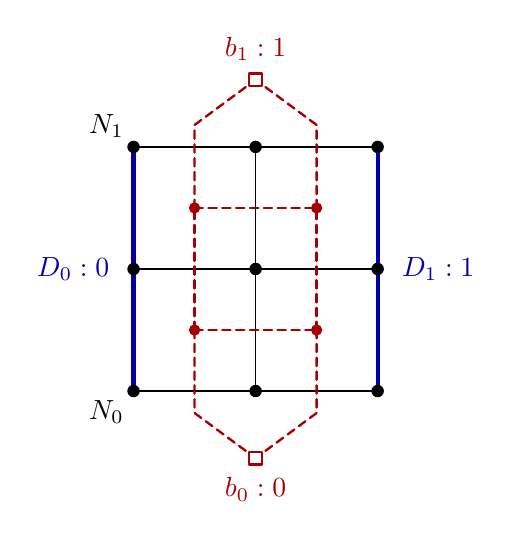
\begin{tikzpicture}[scale=1.55, line cap=round, line join=round,
    primal/.style={draw=black, line width=.65pt},
    prescribed/.style={draw=blue!65!black, line width=1.5pt},
    dual/.style={draw=red!65!black, densely dashed, line width=.85pt},
    face/.style={circle, fill=red!65!black, inner sep=1.45pt},
    wire/.style={rectangle, draw=red!65!black, fill=white,
                 line width=.9pt, inner sep=2.3pt}]
  \draw[primal] (0,0) grid (2,2);
  \draw[prescribed] (0,0)--(0,2);
  \draw[prescribed] (2,0)--(2,2);

  \draw[dual] (.5,.5)--(1.5,.5);
  \draw[dual] (.5,1.5)--(1.5,1.5);
  \draw[dual] (.5,.5)--(.5,1.5);
  \draw[dual] (1.5,.5)--(1.5,1.5);
  \draw[dual] (.5,.5)--(.5,-.18)--(1,-.55);
  \draw[dual] (1.5,.5)--(1.5,-.18)--(1,-.55);
  \draw[dual] (.5,1.5)--(.5,2.18)--(1,2.55);
  \draw[dual] (1.5,1.5)--(1.5,2.18)--(1,2.55);

  \foreach \x in {0,1,2}
    \foreach \y in {0,1,2}
      \fill[black] (\x,\y) circle (1.45pt);
  \foreach \x in {.5,1.5}
    \foreach \y in {.5,1.5}
      \node[face] at (\x,\y) {};
  \node[wire] at (1,-.55) {};
  \node[wire] at (1,2.55) {};

  \node[left, text=blue!65!black] at (-.12,1) {\(D_0:0\)};
  \node[right, text=blue!65!black] at (2.12,1) {\(D_1:1\)};
  \node[below left] at (0,0) {\(N_0\)};
  \node[above left] at (0,2) {\(N_1\)};
  \node[below, text=red!65!black] at (1,-.63) {\(b_0:0\)};
  \node[above, text=red!65!black] at (1,2.63) {\(b_1:1\)};
\end{tikzpicture}

 \caption{The complementary boundary problems in
 Lemma~\ref{lem:mixed-duality}, shown on a \(2\)-by-\(2\) grid.
 The solid primal graph has prescribed values on \(D_0,D_1\).
 Dashed dual edges crossing the other two boundary arcs end at the two
 separate wired vertices \(b_0,b_1\); duals of the prescribed boundary
 edges are omitted.  The wiring represents the two exterior faces after
 the added source-to-sink edge splits the exterior.}
 \label{fig:mixed-boundary-duality}
\end{figure}

The finite identity will be used on squares whose boundary is an actual
primal circuit.  We first give the compactness fact needed for the lower
conductance bound.

\begin{lemma}[Local harmonic compactness]\label{lem:harmonic-compactness}
Let \(O\) be an open coordinate region in the extracted networks.  Suppose
\(w_m\) is harmonic at every vertex with full star in \(O\), and for every
\(V\Subset O\),
\(\sup_m\mathcal E_m(w_m;V)<\infty\).
Then \(w_m\) is asymptotically equicontinuous on compact subsets of \(O\):
if \(z_m(v_m),z_m(v_m')\) lie in a fixed compact subset and their distance
tends to zero, then
\(\abs{w_m(v_m)-w_m(v_m')}\to0\).
If the values are also locally bounded, every subsequence has a further
subsequence converging locally uniformly in vertex tests to a continuous
function.
\end{lemma}

\begin{proof}
Suppose two close vertex sequences have a common limiting position \(z\).
Choose a closed disk about \(z\) inside \(O\) and let \(M\) bound the energy
in a slightly larger disk.  For an integer \(N\), place \(N\) disjoint
concentric collars of the same relative shape inside that larger disk.
Their radii decrease geometrically, and they are all fixed before taking
the network limit.  In collar \(i\), the circuit-traffic estimate selects
a surrounding circuit \(\gamma_i\) with total variation at most
\(\sqrt{B E_{i,m}}\), where \(E_{i,m}\) is the energy paid in that collar.
The collars, including their fixed small margins, can be disjoint, so
some \(i\) has \(E_{i,m}\le M/N\).

Every vertex in the disk inside that circuit has value between the minimum
and maximum on the circuit.  Indeed all its undetermined vertices are
harmonic, and every component inside reaches the circuit: an original
graph path from such a component to the rest of the connected map must
meet the separating circuit.  The finite maximum principle therefore
bounds the oscillation inside by \(\sqrt{BM/N}\).
For all sufficiently large \(m\), both close vertices lie inside the
smallest of the \(N\) collars.  Let \(m\) tend to infinity and then let
\(N\) increase.  This proves their difference tends to zero.  For a
random \(z\), the collars may be chosen from the countable library by
rational perturbations that keep a common inner disk and the disjoint
margins; their relative shapes remain in one fixed bounded range.

The sequential assertion gives equicontinuity on every compact by
contradiction and compactness of its position set.  The vertex positions
are dense in each compact region up to an error tending to zero, by the
flag mesh and the homeomorphisms.  Choose vertices approaching a countable
dense set, extract their bounded values diagonally, and use the
equicontinuity to extend the limits continuously and uniformly on finite
nets.  This gives the stated local uniform convergence.
\end{proof}

\begin{lemma}[Conductance of an approximating square]\label{lem:square-conductance}
Let \(Q=(0,1)^2\) have closure in an ordinary canonical chart.  There are
simple primal boundary circuits approaching \(\partial Q\), with four
ordered side arcs, for which the primal left-to-right and complementary
dual bottom-to-top conductances satisfy
\[
                C_m^{\rm p}\longrightarrow k_{\rm p},
 \qquad        C_m^{\rm d}\longrightarrow k_{\rm d}.
\]
The complementary dual uses exactly the wiring of
Lemma~\ref{lem:mixed-duality}.
\end{lemma}

\begin{proof}
Embed a cube graph in the canonical sphere with one facial cycle equal to
\(\partial Q\), and pull this embedding back to the reference sphere by
\(T^{-1}\).  The cubic skeleton lift
\cite[Lemma~4.7]{C} gives a subdivided primal cube whose graph
homeomorphism tracks the pulled-back embedding to any fixed accuracy; its facial
cycles and their order are preserved up to one reversal.
The reference homeomorphisms in Proposition~\ref{prop:geometry} have
vanishing projection error, and \(T_m\to T\) uniformly transfers that
tracking to the canonical sphere.  Apply the lift at successively smaller fixed
accuracies and choose their thresholds increasingly.  This gives a simple
primal cycle \(\gamma_m\) with an ordered parametrization approaching
\(\partial Q\) uniformly.  In particular, its inside contains every
compact subset of \(Q\) eventually and lies in every fixed enlargement
of \(\overline Q\).  Let \(G_m^Q\) be the submap consisting of this cycle
and everything inside it.  Its four arcs follow the four square sides
with error tending to zero.  Define \(C_m^{\rm p},C_m^{\rm d}\) as in
Lemma~\ref{lem:mixed-duality}, using unit conductances.

Write \(Q^\epsilon=\{x:\dist(x,\overline Q)<\epsilon\}\).  For an upper
bound, choose a smooth function \(f_\delta\) on a neighborhood
of \(\overline Q\), depending only on the horizontal coordinate, equal to
zero in a strip about the left side and one in a strip about the right
side.  It can be chosen with
\[
 \int_Q\abs{\nabla f_\delta}^2\dd x\longrightarrow1
 \quad\text{as }\delta\downarrow0.
\]
For example, flatten the linear function in strips of width \(\delta\),
use slope \(1/(1-2\delta)\) between them, and smooth the two bends in
smaller strips.  Extend it to a fixed small enlargement \(Q^\epsilon\).
For fixed \(\delta,\epsilon\), every edge of \(G_m^Q\) is eventually
located in \(Q^{\epsilon/2}\).  Apply the recovery clause of
Lemma~\ref{lem:uniform-relaxation} with
\(W=Q^{\epsilon/2}\Subset U=Q^\epsilon\), together with
\eqref{eq:scalar-relaxation}.  It recovers \(f_\delta\) uniformly on
a neighborhood of \(\overline{Q^{\epsilon/2}}\), with limsup energy
on \(Q^{\epsilon/2}\) at most
\(k_{\rm p}\int_{Q^\epsilon}\abs{\nabla f_\delta}^2\dd x\).
The constant-recovery modification after
Lemma~\ref{lem:energy-measures} makes it exactly zero and one on smaller
side strips, with additional energy \(o(1)\).  The boundary arcs lie
in these strips for all large \(m\).  Hence
\[
 \limsup_m C_m^{\rm p}
 \le k_{\rm p}\int_{Q^\epsilon}\abs{\nabla f_\delta}^2\dd x.
\]
Let \(\epsilon\downarrow0\), and then \(\delta\downarrow0\), to obtain
\(\limsup C_m^{\rm p}\le k_{\rm p}\).

For the dual upper bound use the corresponding function of the vertical
coordinate, with the same recovery domains
\(W=Q^{\epsilon/2}\Subset U=Q^\epsilon\).  Thus the full-dual recovery
converges uniformly on a neighborhood of
\(\overline{Q^{\epsilon/2}}\), and its limsup energy on \(Q^{\epsilon/2}\)
is bounded by \(k_{\rm d}\) times its Dirichlet integral over \(Q^\epsilon\).
Apply the constant-recovery modification after
Lemma~\ref{lem:energy-measures} to this full-dual recovery on smaller
bottom and top side strips whose closures lie in \(Q^{\epsilon/2}\)
and in the constant regions of the vertical profile.  It makes the
recovery exactly zero and one there, with additional energy \(o(1)\).
Give an interior face its modified full-dual value and
give each wired vertex its prescribed constant.  A dual edge crossing
one of the two relevant boundary arcs has its other endpoint at a
genuine exterior face of the full map.  The complete star of that face
has diameter tending to zero.  Thus this endpoint is in the smaller
constant side strip for all large \(m\), and the squared difference is
exactly the squared difference to the wired value.  The same face cannot
meet the two separated side strips.  For this fixed \(\epsilon\), all
interior dual edges and these boundary crossing edges eventually lie in
\(Q^{\epsilon/2}\), including their whole
endpoint stars.  Their energy is consequently bounded by the recovered
full-dual energy on \(Q^{\epsilon/2}\).  The identical sequence of fixed
limits, with vertical \(f_\delta\), gives
\(\limsup C_m^{\rm d}\le k_{\rm d}\).

For the lower bound take a subsequence attaining the liminf of either
conductance and its minimizing voltages, clipped to \([0,1]\).
The upper bound just proved gives bounded total energies.
The voltages are harmonic at every undetermined vertex in the submap.
On each compact subset of \(Q\), the boundary is absent for large \(m\),
and all original primal incidences, or all original dual incidences, are
present.  Lemma~\ref{lem:harmonic-compactness} therefore gives a locally
uniformly convergent further subsequence, with continuous limit \(f\).

We verify its prescribed boundary values away from the four corners.
Near the relative interior of a primal prescribed side, extend the
voltage to its fixed value on all exterior vertices.  Locally this
adds no energy: an edge leaving the submap passes through a prescribed
boundary vertex.  Near a prescribed side for the dual problem, extend
the voltage to the wired value on the actual exterior faces.  The
boundary crossing edges in this neighborhood are precisely the edges
to that wired vertex in the complementary problem.  Other exterior
edges have both endpoints at the same value.  Whole-face mesh and the
positive distance from the corners ensure that no other side enters
this neighborhood.  Thus the extended energies in a fixed neighborhood
are bounded by the already bounded submap energies.

Fix a point in the relative interior of such a side.  Use \(N\) disjoint
fixed circular collars centered there, as in
Lemma~\ref{lem:harmonic-compactness}, within the neighborhood just
described.  Every surrounding circuit visits the exterior side of the
approximating boundary.  Its Jordan interior contains an inner disk;
a ray from a point of that disk on the exterior side to the far exterior
must cross the circuit.  The crossing has a fixed positive distance
from the limiting side, so vanishing mesh supplies an exterior vertex
of the circuit.  That vertex has the prescribed value.  One of the
\(N\) circuits has variation at most \(\sqrt{BM/N}\).  The maximum
principle inside it applies to all undetermined vertices; the other
vertices there have the prescribed constant value.  It bounds their
difference from that constant by \(\sqrt{BM/N}\).  First take the network
limit and then increase \(N\).  This proves that \(f\) extends
continuously to the prescribed value on each relative side interior,
uniformly on its compact subsegments.

For \(V\Subset Q\), all edges located in \(V\) belong to the submap
eventually, for either network.  Extend the minimizing function arbitrarily
outside the submap; no edge in this inner test sees the extension.
The lower relaxation bound and \eqref{eq:scalar-relaxation} give
\[
 k_{\rm p}\int_V\abs{\nabla f}^2\dd x
       \le\liminf_m C_m^{\rm p}
\]
in the primal case, and the corresponding inequality with \(k_{\rm d}\)
in the dual case.  Exhausting \(Q\) puts \(f\) in \(H^1(Q)\) when the
liminf is finite.  In the primal case its boundary values are zero and
one on the relative interiors of the left and right sides.  The Sobolev
line property and Cauchy--Schwarz on horizontal slices give
\(\int_Q\abs{\nabla f}^2\ge1\).  More explicitly, on
\(y\in[\eta,1-\eta]\) the boundary convergence makes
\(f(a,y)\) uniformly close to zero and \(f(1-a,y)\) uniformly close
to one for small \(a>0\).  For almost every such \(y\),
\[
 \int_a^{1-a}\abs{\partial_x f(x,y)}^2\dd x
 \ge \frac{\abs{f(1-a,y)-f(a,y)}^2}{1-2a}.
\]
Integrate, let \(a\downarrow0\), and then \(\eta\downarrow0\).
The dual problem has the same calculation on vertical slices.
Consequently both liminfs are at least their stated scalars.  Together
with the upper bounds this proves the lemma.
\end{proof}

\begin{proof}[Proof of Theorem~\ref{thm:conductivity}]
Lemma~\ref{lem:energy-tensor} identifies the two reference relaxations
with the scalar integrals \(k_{\rm p}\) and \(k_{\rm d}\).
Equation~\eqref{eq:coordinate-relaxation} puts these integrals in the
same canonical coordinate, and \eqref{eq:equal-dual-scalars} equates
their positive constants.  Apply Lemma~\ref{lem:mixed-duality} to every
submap in Lemma~\ref{lem:square-conductance}.  Its exact identity and
the two limits give
\[
                  k_{\rm p}k_{\rm d}=1.
\]
Thus \(k_{\rm p}=k_{\rm d}=1\).

For a continuous function outside \(H^1_{\rm loc}\), local finiteness
is ruled out by Lemma~\ref{lem:energy-bounds}.  For a continuous
\(H^1_{\rm loc}\) function with infinite integral, inner exhaustion
and its lower bound give infinite relaxed energy.  This completes
\eqref{eq:unit-conductivity} for every continuous input.

Proposition~\ref{prop:geometry}(iv) supplies ordinary chart interiors
from two rerootings covering the canonical sphere.  Each carries the
formula just proved, by Proposition~\ref{prop:sphere-support} in its
own marked marginal and by \eqref{eq:coordinate-relaxation}.  On
overlaps these are restrictions of the same finite-network relaxation,
as in Lemma~\ref{lem:uniform-relaxation}.  The Radon measure property
therefore patches their common Dirichlet density across a finite
subcover of each compact test.  This proves the sphere statement,
including at points omitted by one of the rootings.  The lower and
recovery assertions are Lemma~\ref{lem:uniform-relaxation} with the
now identified value.  Since the finite product has fixed the value
to one on every further extraction, the coefficient is independent
of the extraction.
\end{proof}

\section{Four-point potentials}\label{sec:green}

The conductivity theorem identifies local energies of uniformly convergent
functions.  Point-source voltages have no bounded total energy in the
limit, so we first obtain bounds away from their poles.  We then use local
energy replacements to determine their harmonic limit and its flux.

Throughout this section \(m=2n\), and the network is the full primal
network on the sphere.  Its vertex positions are \(z_n(v)\) from
Proposition~\ref{prop:geometry}.  Choose an edge position \(z_n(e)\) on
each canonical edge arc.  For a spatial Borel set \(U\), write
\[
 \mathcal E_n^0(w;U)
   =\sum_{e:\,z_n(e)\in U}(d_e w)^2.
\]
This is the notation \eqref{eq:local-network-energy} in the canonical
coordinate.  The choice of edge positions has no effect on inner limits.

Let \(\mathsf a_n,\mathsf b_n\) be distinct vertices.  The unit-current voltage is a
solution of
\begin{equation}\label{eq:point-current}
                   Q_n u_n=\delta_{\mathsf a_n}-\delta_{\mathsf b_n},
\end{equation}
where \(Q_n\) is the graph Laplacian of Lemma~\ref{lem:normalization}.
It exists and is unique up to a constant because the graph is connected.
For every vertex function \(w\), summation by parts gives
\begin{equation}\label{eq:point-current-weak}
 \mathcal E_n^0(u_n,w)=w(\mathsf a_n)-w(\mathsf b_n).
\end{equation}
Equivalently, \(u_n\) minimizes
\begin{equation}\label{eq:source-functional}
 \mathcal J_n(v)
     =\mathcal E_n^0(v)-2\bigl(v(\mathsf a_n)-v(\mathsf b_n)\bigr).
\end{equation}
Indeed, for any \(v\),
\[
 \mathcal J_n(v)-\mathcal J_n(u_n)
 =\mathcal E_n^0(v-u_n)
   +2\mathcal E_n^0(u_n,v-u_n)
   -2\bigl((v-u_n)(\mathsf a_n)-(v-u_n)(\mathsf b_n)\bigr)
 =\mathcal E_n^0(v-u_n).
\]
This identity fixes the normalization of the flux calculation below.

Identify the canonical Riemann sphere with the unit round sphere in
\(\R^3\), and write
\(\operatorname{ch}(z,w)=\abs{z-w}_{\R^3}\) for chordal distance.
For distinct \(x,y,z_0\), define on \(\Sph\setminus\{x,y\}\)
\begin{equation}\label{eq:round-voltage}
 U_{x,y;z_0}(z)
   =\frac1{2\pi}
       \log\frac{\operatorname{ch}(z,y)\operatorname{ch}(z_0,x)}
                     {\operatorname{ch}(z,x)\operatorname{ch}(z_0,y)}.
\end{equation}
It vanishes at \(z_0\).  The ratio is the modulus of a conformal cross
ratio, so the function does not depend on the choice of stereographic
coordinate.

\begin{theorem}[Four-point voltage convergence]\label{thm:four-point}
Fix a joint extraction on which
Proposition~\ref{prop:geometry}, Theorem~\ref{thm:network-bounds}, and
Theorem~\ref{thm:conductivity} hold.  Let
\(\mathsf a_n,\mathsf b_n,\mathsf c_n,\mathsf d_n\) be vertex
sequences whose canonical positions converge respectively to four
pairwise distinct points \(x,y,z,z_0\).  Normalize the solution of
\eqref{eq:point-current} by \(u_n(\mathsf d_n)=0\).  Then, for every compact
\(K\subset\Sph\setminus\{x,y\}\),
\begin{equation}\label{eq:local-voltage-convergence}
 \sup_{v:\,z_n(v)\in K}
    \abs{u_n(v)-U_{x,y;z_0}(z_n(v))}\longrightarrow0.
\end{equation}
An empty supremum in \eqref{eq:local-voltage-convergence} is assigned
the value zero.
In particular,
\[
 u_n(\mathsf c_n)-u_n(\mathsf d_n)\longrightarrow
 \frac1{2\pi}
       \log\frac{\operatorname{ch}(z,y)\operatorname{ch}(z_0,x)}
                     {\operatorname{ch}(z,x)\operatorname{ch}(z_0,y)}.
\]
The assertion holds for any such varying vertex sequences on the
extracted sample.
\end{theorem}

\subsection{Bounds away from the current sources}

\begin{lemma}[Local bounds for point-source voltages]\label{lem:voltage-bounds}
Under the assumptions of Theorem~\ref{thm:four-point}, let
\(O=\Sph\setminus\{x,y\}\).  For every compact \(K\subset O\) there
are finite sample-dependent constants \(M_K,M_K'\) such that, eventually,
\[
 \sup_{v:\,z_n(v)\in K}\abs{u_n(v)}\le M_K,
 \qquad
 \mathcal E_n^0(u_n;K)\le M_K'.
\]
Here the energy on \(K\) counts edges located in \(K\).
Every subsequence has a further subsequence converging locally uniformly
in vertex tests on \(O\) to a continuous function.
\end{lemma}

\begin{proof}
For a vertex \(v\), there is a path from \(v\) to \(\mathsf a_n\) on which the
voltage is at least \(u_n(v)\).  To prove this, let \(S\) be the component
of \(v\) in the induced superlevel graph
\(\{w:u_n(w)\ge u_n(v)\}\).  If \(\mathsf a_n\notin S\), connectivity supplies
a boundary edge, and every boundary difference from \(S\) to its
complement is strictly positive.  Consequently
\[
 \sum_{w\in S}(Q_nu_n)(w)
   =\sum_{\substack{e=\{w,w'\}\\w\in S,\ w'\notin S}}
                   (u_n(w)-u_n(w'))>0,
\]
whereas \eqref{eq:point-current} makes the left side nonpositive.
This is a contradiction.  The sublevel argument with signs reversed
gives a path from \(v\) to \(\mathsf b_n\) with voltage at most \(u_n(v)\).

For real \(\alpha<\beta\), let \(T\) clip a number to
\([\alpha,\beta]\), and put \(D=\beta-\alpha\).  Monotonicity and the
one-Lipschitz property of \(T\) give on every edge
\[
 (d_e Tu_n)^2\le d_e u_n\,d_e Tu_n.
\]
Using \eqref{eq:point-current-weak},
\begin{equation}\label{eq:clipped-energy}
 \mathcal E_n^0(Tu_n)
 \le \mathcal E_n^0(u_n,Tu_n)
 =Tu_n(\mathsf a_n)-Tu_n(\mathsf b_n)\le D.
\end{equation}

Fix concentric inner and outer coordinate disks and a circular collar
between them surrounding the inner disk, with the entire closed outer
disk contained in \(O\).  For large \(n\), both source vertices lie
outside the outer disk.
Choose any two vertices in the inner disk and let their voltages be
\(\alpha\le\beta\).  The superlevel path from the higher vertex to
\(\mathsf a_n\) and the sublevel path from the lower vertex to \(\mathsf b_n\) meet every
surrounding circuit in the collar.  The intersections are graph vertices,
because these paths and circuits belong to the same embedded network.
At the two intersections the clipped voltage takes the values \(\beta\)
and \(\alpha\).  Its total variation on each such circuit is at least \(D\).

Theorem~\ref{thm:network-bounds} supplies a circuit law with
\(\sum_e\tau(e)^2\le B\).  The expectation below is only over that
finite-network circuit law.  By \eqref{eq:clipped-energy},
\[
 D\le
 \EE\!\left[\sum_{e\in\gamma}\abs{d_e Tu_n}\right]
 =\sum_e\tau(e)\abs{d_e Tu_n}
 \le \sqrt{B\,\mathcal E_n^0(Tu_n)}
 \le\sqrt{BD}.
\]
Thus the voltage oscillation in the inner disk is at most \(B\),
independently of the total energy of \(u_n\).

The punctured sphere \(O\) is connected.  Cover a compact \(K\subset O\)
and finitely many paths joining it to \(z_0\) by finitely many such disks,
with consecutive disks overlapping.  Vertices occur in each overlap for
all large \(n\), by the vanishing mesh in
Proposition~\ref{prop:geometry}.  Chaining the oscillation bounds and using
\(u_n(\mathsf d_n)=0\), \(z_n(\mathsf d_n)\to z_0\), gives the asserted bound \(M_K\).
The chart cover in Proposition~\ref{prop:geometry}(iv) allows these disks
at every point of \(O\), including a point omitted by one rooting.  Under
the uniform conformal or anticonformal comparison, sufficiently small
fixed round collars contain and are contained in reference collars of
comparable relative shape.  Their fixed-test circuit bounds therefore
apply in the canonical coordinate.

Choose a slightly larger compact neighborhood \(K'\subset O\) of \(K\).
For large \(n\), both endpoints of every edge located in \(K\) lie in
\(K'\).  Clip \(u_n\) to an interval containing all its values on \(K'\).
This clipping leaves those edge differences unchanged.
\eqref{eq:clipped-energy} bounds their total energy by the finite length
of that interval, giving \(M_K'\).

For each fixed \(V\Subset W\Subset O\), both moving source vertices
are eventually outside \(\overline W\).  Equation
\eqref{eq:point-current} then makes \(u_n\) harmonic at every vertex
with full star in \(W\).  Apply Lemma~\ref{lem:harmonic-compactness}
on \(W\), using the local bounds just proved, to obtain compactness on
\(V\).  A countable exhaustion by such buffered pairs and a diagonal
extraction give the final subsequential compactness assertion on \(O\).
\end{proof}

\subsection{Local energy convergence and harmonicity}

Take a subsequence furnished by Lemma~\ref{lem:voltage-bounds}, and write
\(u\) for its locally uniform limit on \(O\).  Associate to its finite
voltages the edge energy measures
\[
             \xi_n=\sum_e(d_eu_n)^2\delta_{z_n(e)}.
\]
Their masses are bounded on every compact subset of \(O\).  A diagonal
vague extraction on this locally compact space gives a Radon measure
\(\xi\) on \(O\).

\begin{lemma}[No local energy defect]\label{lem:no-energy-defect}
On this extraction, \(u\in H^1_{\rm loc}(O)\), \(u\) is harmonic on \(O\),
and
\begin{equation}\label{eq:no-energy-defect}
                         \xi=\abs{\nabla u}^2\dd x
\end{equation}
in every conformal chart of \(O\).  Hence the edge energies converge on
every relatively compact continuity set of the measure on the right.
\end{lemma}

\begin{proof}
We first justify the lower measure bound with the necessary outer room.
Fix a compact \(K\) inside a relatively compact open \(D\subset O\).
Choose \(K\subset V\Subset W\Subset D\), with \(V,W\) open and
\(\xi(\partial W)=0\).  Such a \(W\) can be chosen among distance
neighborhoods with sufficiently small radius: the boundaries are disjoint
as the radius varies, and a finite measure gives positive mass to at most
countably many of them.  The local uniform convergence and the lower
bound of Lemma~\ref{lem:uniform-relaxation} give
\[
 \mathcal R(u,V)
 \le\liminf_n\mathcal E_n^0(u_n;W)=\xi(W)<\infty.
\]
The equality uses vague convergence on the relatively compact continuity
set \(W\).  These choices around each compact set and
Lemma~\ref{lem:energy-bounds} put \(u\) in \(H^1_{\rm loc}(O)\).
Theorem~\ref{thm:conductivity} now identifies
\(\mathcal R(u,V)=\int_V\abs{\nabla u}^2\).  Thus
\[
 \int_K\abs{\nabla u}^2\dd x\le\xi(D).
\]
Take the supremum over compact \(K\subset D\), and then over relatively
compact \(D\).  This proves
\begin{equation}\label{eq:energy-defect-lower}
                        \abs{\nabla u}^2\dd x\le\xi.
\end{equation}
The continuity set \(W\) is essential here: the open-set Portmanteau
inequality alone has the opposite direction for the desired comparison.

We next use local minimization to obtain the reverse bound and harmonicity.
Work in one Euclidean chart, and let \(B_r=B(z,r)\Subset O\) be a disk
with \(\xi(\partial B_r)=0\).  Let
\(\varphi\in C_c^\infty(B_r)\).  Choose fixed radii
\[
             r<r_1<r_2<r_3<r_4,\qquad B_{r_4}\Subset O.
\]
The function \(u+\varphi\) is continuous and in \(H^1\) on this
buffered disk.  The recovery clause of
Theorem~\ref{thm:conductivity} gives \(w_n\to u+\varphi\) uniformly on a
neighborhood of \(\overline B_{r_3}\) and
\begin{equation}\label{eq:local-recovery-bound}
 \limsup_n\mathcal E_n^0(w_n;B_{r_3})
 \le\int_{B_{r_4}}\abs{\nabla(u+\varphi)}^2\dd x.
\end{equation}
Choose a cutoff \(\theta_n\) equal to one on \(B_{r_1}\) and zero outside
\(B_{r_2}\), with bounded energy for these fixed radii.  Put
\[
                 v_n=\theta_n w_n+(1-\theta_n)u_n.
\]
Extend the recovery arbitrarily where it is multiplied by zero.
All changed edges lie in \(B_{r_3}\) for large \(n\), by the open room
and star mesh.  The transition collar is outside \(B_r\), where
\(\varphi=0\), so \(w_n-u_n\to0\) uniformly there.  Applying the
edge identity \eqref{eq:edge-gluing} to these two functions gives
\begin{equation}\label{eq:local-replacement-bound}
 \mathcal E_n^0(v_n;B_{r_3})
 \le \mathcal E_n^0(w_n;B_{r_3})
       +\mathcal E_n^0(u_n;B_{r_3}\setminus\overline B_r)+o(1).
\end{equation}
Indeed the principal squared differences are bounded by their convex
combination.  The coefficient of an old difference can be nonzero only
outside \(\overline B_r\), since \(\theta_n=1\) on \(B_{r_1}\) and
the mesh is small.  The remaining term has energy bounded by
\(\sup_{\rm collar}\abs{w_n-u_n}^2\mathcal E_n^0(\theta_n)=o(1)\);
its cross term is \(o(1)\) by the bounded old and recovered energies.

Neither source value changes.  The minimizing identity
\eqref{eq:source-functional}, restricted to the changed edges, gives
\(\mathcal E_n^0(u_n;B_{r_3})
 \le\mathcal E_n^0(v_n;B_{r_3})\).
Subtract the old energy on
\(B_{r_3}\setminus\overline B_r\) in
\eqref{eq:local-replacement-bound}.  The difference on the left is
\(\xi_n(\overline B_r)\ge\xi_n(B_r)\), so the result is
\[
                \xi_n(B_r)
                \le\mathcal E_n^0(w_n;B_{r_3})+o(1).
\]
Take \(n\) to infinity.  The left side tends to \(\xi(B_r)\) because
\(B_r\) is a continuity set, and
\eqref{eq:local-recovery-bound} bounds the right side.  Now decrease
\(r_4\) to \(r\), choosing the three intermediate radii afresh between
them at each step.  Each cutoff is used only for a fixed step before
the network limit.  The continuum energy has no mass on the circle
\(\partial B_r\), so
\begin{equation}\label{eq:local-minimality-limit}
       \xi(B_r)\le
         \int_{B_r}\abs{\nabla(u+\varphi)}^2\dd x.
\end{equation}

Set \(\varphi=0\).  Together with
\eqref{eq:energy-defect-lower}, this gives equality of the two measures
on every such disk.  These disks form a cover basis after excluding
at most countably many radii at each center.  The nonnegative measure
\(\xi-\abs{\nabla u}^2\dd x\) vanishes on that basis, hence vanishes
on \(O\).  This proves \eqref{eq:no-energy-defect}.

For \(\psi\in C_c^\infty(B_r)\), use
\(\varphi=t\psi\) in \eqref{eq:local-minimality-limit} and the measure
equality.  Expanding for both signs of \(t\) and letting \(t\to0\)
gives
\(\int_{B_r}\nabla u\cdot\nabla\psi\dd x=0\).
Every point has such a disk, so \(u\) is distributionally harmonic on
\(O\).  Interior harmonic regularity makes it classically harmonic.
Finally, vague convergence to the measure in
\eqref{eq:no-energy-defect} gives convergence on each of its relatively
compact continuity sets.
\end{proof}

The proof used recovery for the particular limiting function \(u\).
This is legitimate pathwise: Lemma~\ref{lem:uniform-relaxation} obtains
its statements for every continuous function from one countable cell
library.  No conditional kernel depending on the subsequently chosen
voltage limit is needed.

\subsection{Unit flux and the logarithmic poles}

\begin{proof}[Proof of Theorem~\ref{thm:four-point}]
Take any subsequence.  Lemma~\ref{lem:voltage-bounds} and a further
vague energy extraction give a locally uniform limit \(u\) on \(O\).
Lemma~\ref{lem:no-energy-defect} makes \(u\) harmonic there and identifies
its local energy measure.  The normalization \(u_n(\mathsf d_n)=0\) and local
uniform convergence imply \(u(z_0)=0\).

Choose a conformal disk about \(x\) whose closure avoids \(y\), with
\(x\) at its Euclidean center.  Let \(\chi\) be a smooth radial function
equal to one on a smaller disk and zero outside a larger disk, with
its transition compactly in the punctured disk.  Choose a closed-buffered
annular domain \(V\Subset O\) containing \(\supp\nabla\chi\) with
clearance from both boundary components.  Its two boundary circles
have zero \(\abs{\nabla u}^2\dd x\)-mass.

Fix \(t\in\R\).  Choose annuli \(V\Subset W\Subset U\Subset O\) by
slightly moving the two boundary radii, and recover \(u+t\chi\) on a
neighborhood of \(\overline W\).  The recovery \(w_n\) satisfies
\begin{equation}\label{eq:flux-recovery}
 \limsup_n\mathcal E_n^0(w_n;W)
       \le\int_U\abs{\nabla(u+t\chi)}^2\dd x.
\end{equation}
For a vertex of the full network put
\[
                  \widehat u_n(v)=u_n(v)+t\chi(z_n(v)).
\]
Take an annular cutoff \(\theta_n\) equal to one on a neighborhood of
\(\overline V\) and zero outside an intermediate annulus compactly
contained in \(W\).  Such a cutoff is obtained by combining two disk
cutoffs; its energy is bounded for these fixed radii.  Define
\[
                  v_n=\theta_n w_n+(1-\theta_n)\widehat u_n.
\]
On both transition collars \(w_n-\widehat u_n\to0\) uniformly.  Wherever
the coefficient \(1-\theta_n\) of an edge difference can be nonzero,
the edge lies outside \(\overline V\) with a margin, where \(\chi\)
is constant on each component.  Thus
\(d_e\widehat u_n=d_eu_n\) on every such edge for all large \(n\).
This uses the clearance from \(\supp\nabla\chi\) and vanishing star mesh.
Outside \(W\),
\(\chi\) is constant on the inner and outer components and
\(\theta_n=0\); hence the changed energy is confined to \(W\).
The source vertex is in the inner component and the sink is in the
outer one, so
\[
                v_n(\mathsf a_n)=u_n(\mathsf a_n)+t,\qquad
                v_n(\mathsf b_n)=u_n(\mathsf b_n).
\]

The edge gluing estimate, with the old part supported outside
\(\overline V\), gives
\[
 \mathcal E_n^0(v_n;W)
 \le \mathcal E_n^0(w_n;W)
       +\mathcal E_n^0(u_n;W\setminus\overline V)+o(1).
\]
The error has energy at most the squared uniform collar discrepancy times
the fixed cutoff energy, and its cross term tends to zero by local energy
bounds.  Minimality of the source functional
\eqref{eq:source-functional} now gives
\[
 \mathcal E_n^0(u_n;W)
       \le\mathcal E_n^0(v_n;W)-2t.
\]
Subtract the displayed old collar energy.  The difference on the left is
\(\xi_n(\overline V)\ge\xi_n(V)\), so the resulting inequality is
\[
                  \xi_n(V)
                  \le\mathcal E_n^0(w_n;W)-2t+o(1).
\]
By Lemma~\ref{lem:no-energy-defect}, the left side converges to
\(\int_V\abs{\nabla u}^2\), since \(V\) is a continuity set.
Use \eqref{eq:flux-recovery}, then shrink \(U\) to \(V\) through annuli
with the same clearance from \(\supp\nabla\chi\).  At each stage the
annuli and cutoffs are fixed before \(n\) tends to infinity.  Absolute
continuity of the continuum energy and the zero mass of the boundary
circles give
\begin{equation}\label{eq:flux-variation}
 \int_V\abs{\nabla u}^2\dd x
 \le\int_V\abs{\nabla(u+t\chi)}^2\dd x-2t.
\end{equation}
Expanding this inequality yields
\[
 0\le
 2t\left(\int_V\nabla u\cdot\nabla\chi\dd x-1\right)
       +t^2\int_V\abs{\nabla\chi}^2\dd x.
\]
It holds for every real \(t\), so the coefficient of \(t\) is zero:
\begin{equation}\label{eq:unit-source-flux}
                     \int\nabla u\cdot\nabla\chi\dd x=1.
\end{equation}
For a cutoff equal to one near \(y\) and zero near \(x\), the replacement
changes the sink value by \(t\) and the source value by zero.
The source term in \eqref{eq:source-functional} then changes by \(+2t\);
the expanded inequality gives flux \(-1\) at \(y\).

We verify that these fluxes determine the only possible singularities.
Choose an outer coordinate disk about \(x\) whose closure excludes \(y\),
and a fixed collar inside it surrounding a smaller disk about \(x\).
For every sufficiently large \(n\), take a surrounding network circuit
in that collar.  Eventually
\(\mathsf a_n\) is in the smaller disk and \(\mathsf b_n\) is outside
the outer disk, hence outside the circuit.
Lemma~\ref{lem:voltage-bounds} bounds the voltages on that collar
uniformly.  Inside the circuit, \(Q_nu_n=0\) except at the positive
source, where \(Q_nu_n=1\).  The minimum principle therefore
bounds every interior voltage from below by the minimum on the circuit.
Passing to the limit bounds \(u\) from below near \(x\).  For \(y\),
choose an outer disk whose closure excludes \(x\) and a collar inside
it surrounding a smaller disk about \(y\), and take a surrounding
network circuit there.  Eventually \(\mathsf b_n\)
is inside its circuit and \(\mathsf a_n\) is outside the outer disk.
The maximum principle then bounds \(u\) from above near \(y\).

We recall the planar isolated-singularity argument at the needed strength.
If \(v\) is a positive harmonic function on a punctured disk, its circular
mean \(M(r)\) satisfies \((rM'(r))'=0\).  Thus
\[
                       M(r)=a\log(1/r)+b,\qquad a\ge0,
\]
where positivity forces the sign of \(a\).  Harnack's inequality on
the fixed-shape annulus \(\{r/2<\abs z<2r\}\) bounds the values on
\(\abs z=r\) by a constant times \(M(r)\), uniformly in small \(r\).
This version of Harnack follows directly from the Poisson kernel on a
finite chain of disks in the annulus.  Hence \(v=O(1+\log(1/r))\).
For each nonzero angular Fourier mode, harmonicity makes its radial
coefficient a linear combination of \(r^j\) and \(r^{-j}\),
\(j\ge1\).  The logarithmic bound forces every \(r^{-j}\) coefficient
to vanish.  The remaining positive-power series is the harmonic Poisson
extension from any fixed smaller circle.  Consequently
\[
                     v(z)=a\log(1/\abs z)+h(z),
\]
where \(h\) extends harmonically through the center.  Applying this to
\(u\) plus a constant near \(x\), and to \(-u\) plus a constant near
\(y\), shows that \(u\) has only logarithmic or removable singularities.

For \(a\log(1/\abs z)\), a radial cutoff equal to one near zero and zero
outside has
\[
 \int\nabla\!\bigl(a\log(1/\abs z)\bigr)\cdot\nabla\chi\dd x
       =-2\pi a\int\chi'(r)\dd r=2\pi a.
\]
The harmonic remainder contributes zero.  Equation
\eqref{eq:unit-source-flux} therefore sets the coefficient at \(x\)
to \(1/(2\pi)\), and the sink flux sets the coefficient at \(y\) to
\(-1/(2\pi)\).

For comparison, the round zero-mean Green kernel has, up to its additive
constant,
\[
                  G_{\rm rd}(z,w)
                  =-\frac1{2\pi}\log\operatorname{ch}(z,w).
\]
Away from \(w\), a radial calculation on the unit sphere gives
\(-\Delta_z G_{\rm rd}(z,w)=-1/(4\pi)\); the preceding local flux is
one at \(w\).  Thus its distributional equation is
\(-\Delta_zG_{\rm rd}(z,w)=\delta_w-(4\pi)^{-1}\dd\mathrm{vol}_{\rm rd}\).
The difference \(G_{\rm rd}(\cdot,x)-G_{\rm rd}(\cdot,y)\) has exactly
the two fluxes and singular coefficients just found.  Subtract it from
\(u\).  The difference extends harmonically across \(x,y\), and a
harmonic function on the compact sphere is constant.  Its value at
\(z_0\) gives precisely \eqref{eq:round-voltage}.

Every subsequence has therefore a further locally uniform subsequence with
the same limit \(U_{x,y;z_0}\).  This proves
\eqref{eq:local-voltage-convergence} along the entire extraction.
Evaluating at \(\mathsf c_n\) gives the asserted four-point value.  The reasoning
applied to arbitrary varying pole and evaluation vertices with the stated
distinct limits, so it proves the claimed pathwise quantifier.
\end{proof}

\section{An approximation estimate at every smaller scale}
\label{sec:compactness}

The electrical estimates of Theorem~\ref{thm:network-bounds} control
each fixed annulus after a threshold which may depend on that annulus
and on the sample.  Spectral compactness requires one estimate valid
at all remaining discrete scales.  We obtain it from the address
estimates and finite contour views of~\cite{P}.  The new ingredients
are a rank estimate with one marked time, a bound on the number of
widely separated times reached by short contour explorations, and a
cover by circuits which avoids the cost of reaching individual
vertices.

For a set \(W\) of original edges, counted with their map
multiplicities, write
\[
 \mathcal E_m(f;W)=\sum_{e\in W}\abs{f(e^+)-f(e^-)}^2.
\]
The choice of orientation \(e^-,e^+\) is immaterial, and a loop
contributes zero.  On a duration-one sphere \(m=2n\), this is the
restriction of \(\mathcal E_n^0\) to \(W\).

An interval used below is a set \(I_m\) of consecutive letter cuts
inside one used block of a protected chart.  Its endpoints are
specified relative to that block, its length divided by \(m\) has a
positive finite limit, and its limiting tour image has compact
clearance inside a larger protected neighborhood.  The chart records
a graph \(G_m^+\) which contains the interval's vertices and all
edges and complete stars in an intermediate neighborhood, and is
itself reconstructed with room inside the larger neighborhood.
These are entries in the countable atlas of
Proposition~\ref{prop:readout-extension}; activation refers to its
strict continuum conditions.

Split \(I_m\) into nested dyadic halves, rounding integer sizes at
each split.  Retain singleton and empty blocks at later levels.  For
a nonempty level-\(j\) block \(I\), define
\[
 (P_j^{I_m}f)(i)=\frac1{\abs I}\sum_{k\in I}f(v(k)),
 \qquad i\in I.
\]
Thus \(P_j^{I_m}\) is the orthogonal projection of the cut-value
function onto level-\(j\) block constants for counting measure; it
is the identity after every block is a singleton.

\begin{theorem}[All-level block approximation]
\label{thm:block-approximation}
From an arbitrary sequence of finite spheres, take a further joint
representation extraction as in Proposition~\ref{prop:geometry}
and Proposition~\ref{prop:readout-extension}, retaining the interval
readouts defined below.  Put \(m=2n\) and
\(p=7/10\).  Simultaneously for the countable protected interval
atlas, the following holds almost surely on activation of an entry
\((I_m,G_m^+)\).  There are finite sample-dependent constants
\(j_*\), \(C\), and \(n_*\) such that, at every index \(n\ge n_*\)
in the extraction, for every function on \(V(G_m^+)\) and every
integer \(j\ge j_*\),
\begin{equation}
\label{eq:block-approximation}
 \frac1m\sum_{i\in I_m}
   \abs{f(v(i))-(P_j^{I_m}f)(i)}^2
 \le C\,2^{-pj} \mathcal E_n^0(f;G_m^+).
\end{equation}
This includes all levels down to and beyond singleton cuts and holds
for all functions on the same event.

In the two-rooting extraction of Proposition~\ref{prop:geometry},
one can choose finitely many activated entries from the two rooted
atlases such that every corner occurrence belongs to at least one
of their intervals, in its corresponding rooted order, for all
sufficiently large \(n\).
\end{theorem}

We first work with the bilateral word and prove a tight bound on the
smallest sufficient \(j_*\).  Only after that probability estimate
will we regard the threshold as a local readout and transfer
almost-sure finiteness of its extracted limit on activation to sphere charts.

\subsection{Selected words and the address estimates}

Let \(\PP_m^W\) be the product law on bilateral inventory words.
The two burger types, their two rigid orders, and the flexible
order have probabilities
\[
 \frac14,\quad\frac14,\quad
 \frac{2-\sqrt2}{4},\quad\frac{2-\sqrt2}{4},\quad
 \frac{\sqrt2-1}{2},
\]
respectively.  An order consumes the freshest allowed burger.
Resolve flexible orders using the bilateral matching.  The subscript
records the time unit \(m\), not a change of the iid letter law.
The two resolved scalar contours are \(Z^1,Z^2\); their increments
are not asserted independent.  These are the FK-Ising probabilities
of \cite[Proposition~3.1]{C}.  Work in an ordinary bilateral contour
coupling with its reference tour projection; extra field coordinates
use the attachment convention of Proposition~\ref{prop:readout-extension}.
We use a
\emph{scalar link} only for a pair of integer cuts \(s,t\) satisfying
\[
 Z^c(s)=Z^c(t)=\min_{[s\wedge t,s\vee t]}Z^c
 \quad\text{for one }c\in\{1,2\}.
\]
Links can have arbitrary chronological duration.  A time jump is
an arbitrary pair of cuts whose distance is bounded as specified
below.  Put
\[
 r_m(x)=m e^{-x},\qquad
 \vartheta=\frac12+\frac2{\gamma^2}=\frac76.
\]
Every sequential statement in this subsection has
\begin{equation}
\label{eq:selected-units}
 N=N_m\longrightarrow\infty,\qquad
 r_m(bN)\longrightarrow\infty
\end{equation}
for the fixed upper log-range constant \(b>1\).

We record the selection protocol because it will also allow a union
over many levels.  Fix a compact starting window in time units, a
spatial compactness and positive-clearance cutoff, and
\(\sigma_m\downarrow0\) bounding every used seed unit divided by \(m\).
For any fixed
loss \(\epsilon>0\), the preselection construction of
\cite[Section~11]{P} supplies a master event \(\mathcal T_m\),
deterministic enclosures \([-C_d m,C_d m]\), and a deterministic
\(D_m^{\max}\to\infty\).  Its failure probability on the fixed
cutoff is at most \(2\epsilon+o(1)\).  On \(\mathcal T_m\),
simultaneously for \(d\le D_m^{\max}\), every exploration of at most
\(d\) links or jumps of size at most \(dm\) from the starting
window remains in the \(d\)th enclosure.  If its jumps have size
at most \(d\sigma_m m\), all its projected points are within a
deterministic \(\chi_m\downarrow0\) of its base.  This includes
first- and last-return witnesses.  For each fixed \(d\), the
bilateral protected-window result \cite[Proposition~4.9]{C},
after a deterministic compact cutoff, gives the vanishing flag
mesh and exact complete stars needed for the fixed intermediate
neighborhood on that enclosure.  Include its eventual conclusion
with a further prescribed summable loss before selection.
Slowing \(D_m^{\max}\) makes these conclusions simultaneous as well.

A selected law \(\mathbb Q_m\) in this section is supported on
\(\mathcal T_m\) and the stated clearance cutoff.  Its raw-word
marginal satisfies
\begin{equation}
\label{eq:selected-density}
 \frac{d\mathbb Q_m^W}{d\PP_m^W}\le e^{\kappa_m},
 \qquad \kappa_m=o(N).
\end{equation}
Finite lists may be randomized functions of the word and of the
coupled environment.  To apply the companion on its augmented
probability space, give the reference word the selected law's
conditional selector kernel given that word.  This kernel can be
realized by an independent uniform variable; the augmented reference
still has word marginal \(\PP_m^W\), and the full augmented density
is the density in~\eqref{eq:selected-density}.  The selected environment
and bases precede the independent viewing level or seed mesh.
Seed-specific lists may then use their seed levels; their complete
union of positions and access witnesses precedes the independent
chronological address grid.  Subsequent
finite-list cutoffs may grow only along a slower diagonal below
\(D_m^{\max}\).  These are the hypotheses on every selected law
below; we will not transfer a fresh high-probability master event
through~\eqref{eq:selected-density}.

Here is the quantitative address input.  In an enclosure of length
\(h_m^{\mathrm{enc}}=c_{\mathrm{enc}}m\), fix an integer \(R\ge8\), put
\(\ell_R=\log R\), and use generations
\(0\le k\le J_R=\lfloor bN/\ell_R\rfloor\) of cells of width
\(\delta_k=h_m^{\mathrm{enc}}R^{-k}\).  There are \(h_{\mathrm b}\)
distinguished bases marked through \(J_R\).  Use distinct probe
generations.  At each probe generation,
every endpoint and intermediate point in each access chain from
a distinguished base is
marked through that generation; its links are scalar links or
jumps of size at most \(K\delta_k\).  The fixed \(K\) also bounds
the marker and edge entries in every probe list.  Include all distinguished
base entries in the list at terminal generation \(J_R\), merging
them into an existing list there or adding that generation as one
probe.  Enlarge \(K\) to bound the marker and edge entries in this
augmented list as well.  Let \(P_N\) count the resulting distinct
probes and \(M_{\rm term}\) count all marker entries, so
\(M_{\rm term}\le KP_N\).  The count below fixes these augmented
probe depths; in our applications they are determined by an
independent mesh phase held as side information.  The entire
augmented marker system is chosen before the independent
\(\Xi\sim\operatorname{Unif}[0,h_m^{\mathrm{enc}})\) translates the nested grids.

At generation \(k\), let \(m_k\) be the number of occupied cells,
\(b_k\) the number containing a base, and \(D_k\) the number of jump
entries split between distinct cells.  For each color, project every
active recorded chord of that color to the cells containing its endpoints and take
all occupied cells, including isolated ones, as vertices; these graphs
exclude jumps, as in \cite[Definition~10.6 and Lemma~10.7]{P}.
Define graph rank as the number of vertices minus the number of
connected components, so projected loops and repeated edges add no
rank, and let \(e_k\) be the sum of the two color ranks.  Write
\[
 T_{\rm occ}=\sum_k m_k,\qquad R_{\rm rk}=\sum_k e_k.
\]

\begin{proposition}[Address input from the companion]
\label{prop:address-input}
For the marker systems just described, with fixed \(b,R,K\), the
following statements hold.
\begin{enumerate}[label=(\roman*)]
\item If \(c_k\) is the number of components of the union of the
two colored graphs, then
\[
 c_k\le b_k+D_k,\qquad e_k\ge m_k-c_k.
\]
Moreover
\[
 \EE_\Xi\sum_kD_k\le C_{K,R}M_{\rm jump}.
\]
If the bases lie in an interval of length \(C r_m(N)\), then
\(\EE_\Xi\sum_{k\le N/\ell_R}(b_k-1)\le C_{C,R}\).
\item For each \(\varepsilon>0\), a fixed sufficiently large \(R\)
gives, with conditional grid probability at least \(7/8\), disjoint
regular sampling slots after deletion of at most
\(C_RM_{\rm term}+\varepsilon T_{\rm occ}\) node occurrences.
For each sufficiently small fixed \(\varepsilon>0\), \(R\) and
the deletion tolerances may be fixed so that every such code
\(\mathfrak c\) obeys
\begin{equation}
\label{eq:fixed-code-charge}
 \PP_m^W\{\mathfrak c\text{ is realized}\}
 \le
 \exp\{-\vartheta\ell_R R_{\rm rk}
       +\varepsilon\ell_R T_{\rm occ}
       +C_{R,\varepsilon}M_{\rm term}\}.
\end{equation}
Realization includes all its actual chord constraints.  The bound
is uniform in the fixed grid displacement and in the exact
chord endpoints inside the recorded cells, once the minimum
sampling radius diverges.
\item For each fixed displacement and fixed augmented distinct
probe depths, and every \(0<\eta\le K\), the number of decorated codes with
occupancy \(T_{\rm occ}=t\) is at most the exponential of
\begin{equation}
\label{eq:address-count}
 (\ell_R+C_0+\eta)t
 +K P_N\log(K/\eta)+C P_NK\log(K+1)+O(1).
\end{equation}
If the depth list itself is encoded, add
\(\log\binom{J_R+1}{P_N}\); our independent mesh phases are
instead held as side information.
\item Let \(\Delta(\Xi)\) count generations at which the partition
of the active markers into shifted cells differs from the
grid-independent partition obtained by joining consecutive active
positions with gap \(<\delta_k\).  Then
\[
 \EE_\Xi[\Delta(\Xi)\mid\text{markers}]
 \le \frac{2R}{R-1}M_{\rm term}.
\]
At a generation with equal partitions the entire colored graph
and its base labels agree up to cell names.
\end{enumerate}
For \(P_N=O(N/L)\), take the error tolerances and \(R\) fixed first,
then \(N\) and the minimum units to infinity with \(L\to\infty\)
and \(L=o(N)\).  The terminal, jump, and structural errors above
are \(o(N)\) for every fixed \(K\).  One may subsequently let
\(K=K_m\to\infty\) sufficiently slowly, with
\[
 \frac{K_m\log(K_mL)}{L}\longrightarrow0,\qquad
 \frac{K_m\log(2\widehat C_m)}{L}\longrightarrow0,
\]
where \(2\widehat C_m m\) is a growing enclosure length, and with
the composed exploration depth below \(D_m^{\max}\).
The second condition pays for its extra address ancestors.  The
integrated jump error remains \(o(N)\), and each previously fixed
minimum-unit threshold is retained.
\end{proposition}

\begin{proof}
The projected rank and jump inequalities are the spanning-forest
and displaced-grid estimates in~\cite[Section~10]{P}.
The fixed-code estimate is \cite[Proposition~10.15]{P}; its proof
charges a left and right fresh slot for each monochrome rank and
gives the coefficient \(\vartheta=1/2+2/\gamma^2\).
The decorated address count is \cite[Lemma~10.13]{P}: distinct
depths give \(\sum_p m_{k_p}\le T_{\rm occ}\), and the terminal
base list supplies every base's coarser address.  The regular-slot
deletion bound and grid-partition estimate are the corresponding
lemmas in the same section.  Its sparse-diagonal remark gives the
list and jump order of limits; the extra-ancestor estimate in the
proof of \cite[Lemma~11.6]{P} gives the growing-enclosure condition.
In these formulas a generation has log width
\(\ell_R\); this accounts for every conversion between sums over
generations and log lengths.
\end{proof}

We need a packing consequence also at the order of limits in which
the probe stride is held fixed while \(m\) grows.  For \(k\ge1\),
let \(\mathcal R_{m,k}(x)\) be all times reached from the selected
bases by at most \(k\) scalar links or jumps, each jump of size at
most \(k r_m(x)\).  The whole access chain is included.  Bilateral
recurrence below each fixed scalar height makes this set finite.
It is increasing in \(k\), and
\(\mathcal R_{m,k}(x)\subset\mathcal R_{m,k}(y)\) for \(y\le x\).
Define
\[
 \Pi_{m,k,H}(x)=
 \max\{\abs A:A\subset\mathcal R_{m,k}(x),\
       \abs{s-t}>H r_m(x)\ \text{for }s\ne t\text{ in }A\}.
\]

\begin{lemma}[Truncated packing at a typical level]
\label{lem:truncated-packing}
Use the selected protocol above with a fixed number of bases.
Let \(\mathcal I_N\subset[a_-N,bN]\), with fixed \(a_->1\), be
a deterministic log interval of length at least \(cN>0\), and let \(Y\) be uniform on
\(\mathcal I_N\), independently after the selected environment.
Then there is \(C_{\rm pack}<\infty\), independent of each fixed
\(k,M\), such that
\begin{equation}
\label{eq:truncated-packing}
 \sup_{k,M\ge1}\ 
 \lim_{H\to\infty}\limsup_m
 \EE_{\mathbb Q_m}\min\{\Pi_{m,k,H}(Y),M\}
 \le C_{\rm pack}.
\end{equation}
\end{lemma}

\begin{proof}
Choose fixed address parameters within
Proposition~\ref{prop:address-input} so that
\[
 \delta=\vartheta-1-\varepsilon-\frac{C_0+\eta}{\ell_R}>0.
\]
Fix \(k,M\) and a log stride \(L>2\ell_R\).  Sample an independent
translation of a stride-\(L\) mesh in \(\mathcal I_N\).  At each
seed choose a maximum-cardinality \(H\)-packing truncated at \(M\), with all
access witnesses.
Use a fixed measurable ordering of the finite reachable set, and
keep the independent mesh phase as side information in the code count.
Round a seed \(y\) up to generation \(\lceil y/\ell_R\rceil\),
discarding the final incomplete generation if needed.  The seed
depths are distinct because \(L>2\ell_R\).  The terminal base-list
augmentation adds at most one probe and \(h_{\mathrm b}\) fixed
entries, so \(P_N=O(N/L)\) and \(K=O(kM+h_{\mathrm b})\), with
constants allowed to depend on the fixed enclosing depth.
Only then sample the chronological address-grid displacement.
These lists have exactly the order and the form in
Proposition~\ref{prop:address-input}.

We first bound their occupation for this \emph{fixed} \(L\).
Markov's inequality in part (i) gives a set of grid displacements
of fixed positive conditional probability on which
\(\sum D_k\le C_KN/L+O(1)\).  Intersect it with the regular-slot
event, retaining a fixed positive probability.  Use
\(e_k\ge m_k-h_{\mathrm b}-D_k\) in
\eqref{eq:fixed-code-charge} and sum the codes by
\eqref{eq:address-count}.
All terminal and decoration terms at fixed \(K,L\) are
\(O_K(N/L)+O(1)\).  Let \(\mathsf F_t(\Xi)\) be the existence
of a realized regular code with this jump bound and occupancy \(t\).
Uniformly in the displacement,
\begin{equation}
\label{eq:fixed-stride-occupation}
 \log\PP_m^W(\mathsf F_t(\Xi))
 \le -\delta\ell_Rt+
       \bigl[\vartheta h_{\mathrm b}b+O_K(L^{-1})\bigr]N+O(1).
\end{equation}
The constants in the leading term are independent of \(K\).
This calculation retains the terminal errors explicitly; the
asymptotic occupancy statement with \(L=L_m\to\infty\) alone would
not justify the present order of limits.

For two displacements, each cell of one grid meets at most two
cells of the other, hence \(T_{\rm occ}(\Xi)\le
2T_{\rm occ}(\Xi')\).  If the maximum occupancy over displacements
is large, it is at least half as large on every displacement,
including the fixed positive fraction just used.  Integrate
\eqref{eq:fixed-stride-occupation} over the grid and sum over \(t\).
Then apply~\eqref{eq:selected-density}.  It follows that, for a
constant \(C_1\) independent of \(K\), the total log occupation
is at most
\[
 [C_1+O_K(L^{-1})]N
\]
with \(\mathbb Q_m\)-probability tending to one.  The same bound
applies to the occupation restricted to \(\mathcal I_N\).

Here is the conversion to packing, which is the mechanism of
\cite[Lemma~11.4]{P}.  A list chosen at a seed \(y\) remains
reachable throughout the coarser interval \([y-L,y]\).
Use generation \(\lceil x/\ell_R\rceil\) boxes on each continuous
log cell, trimming incomplete endpoint cells.  They are active
throughout \([y-L,y]\) for a seed rounded as above, and their
integrated occupation is at most \(\ell_R T_{\rm occ}\).
If these boxes at level \(x\) have diameter at most
\(c_{\rm box}r_m(x)\), then its chosen terminals stay in distinct
boxes throughout that interval whenever
\(H e^{-L}>2c_{\rm box}\).  Thus the truncated seed count
contributes at least \(L\) times that count to integrated
occupation, apart from the two end intervals and a fixed-width
endpoint strip.  Averaging the
independent mesh translation turns the seed sum into the uniform
integral on \(\mathcal I_N\).  On the occupation-exception event,
bound the truncated packing by \(M\).  Dividing by
\(\abs{\mathcal I_N}\), the end error is at most
\(O(M(L+\ell_R)/\abs{\mathcal I_N})\).  First let \(m\to\infty\) for fixed
\(H,L,k,M\); then take \(H\to\infty\) and
\(L=L(H)\to\infty\) slowly with \(He^{-L}>2c_{\rm box}\).
The term \(O_K(L^{-1})\) vanishes for each fixed \(k,M\), and
the limiting bound is independent of them.  This proves
\eqref{eq:truncated-packing}.
\end{proof}

\begin{lemma}[Few separated times at bounded reach]
\label{lem:reachable-packing}
Fix \(a_0>1\), \(c_0,C_0,\zeta>0\), and a finite integer \(d\).
Under the selected protocol with \(r_m(a_0N)\to\infty\), there
is no sequence of selected laws supported on the existence of
more than \(e^{\zeta N}\) times in the starting window, pairwise
separated by at least \(c_0r_m(N)\), with one common member from
which every member is reached by at most \(d\) scalar links or jumps of size at most
\(C_0r_m(a_0N)\).
\end{lemma}

\begin{proof}
Choose fixed \(1<\alpha<\beta<a_0\) and apply
Lemma~\ref{lem:truncated-packing} with one selected base and
\(\mathcal I_N=[\alpha N,\beta N]\).  For every \(x\in\mathcal I_N\),
the proposed jumps divided by \(r_m(x)\) are at most
\(C_0e^{-(a_0-\beta)N}\), while the proposed separation divided
by \(r_m(x)\) is at least \(c_0e^{(\alpha-1)N}\).  For a fixed
enlargement of \(d\), the proposed list is therefore contained
in \(\mathcal R_{m,k}(x)\) and is an \(H\)-packing for every
fixed \(H\), eventually uniformly in \(x\).  Select the base
and only \(M\) terminals with their witnesses before the grids.
On the asserted event the truncated packing equals \(M\) for
every fixed \(H,M\) and all large \(m\).  Taking the limits in
\eqref{eq:truncated-packing} and then choosing
\(M>C_{\rm pack}\) is a contradiction.
\end{proof}

The other new use of the address budget replaces many nearby bases
by one base and a wider range of smaller scales.  For a connected
component \(C\) of the union of two colored graphs, the sum of the
ranks of their restrictions to \(C\) is at least \(\abs C-1\).
Call it \emph{acyclic} when equality
holds and say it has a \emph{rank cycle} when the rank is at least
\(\abs C\).

\begin{lemma}[One-base rank credit on a wide range]
\label{lem:one-base-credit}
There is a fixed \(B>2\) with the following property.  Use a
sparse address system from Proposition~\ref{prop:address-input}
with one base, upper range \(BN\), and selected
law~\eqref{eq:selected-density}.  Fix \(1<a\le2\) and any
deterministic \(\eta_m\downarrow0\).  The probability that the
projected component containing the base has a rank cycle at all
but \(\eta_mN\) generations with log level
\(k\ell_R\in[aN,BN]\) tends to zero.
\end{lemma}

\begin{proof}
The base is marked at every generation, so \(b_k=1\) and
\(m_k\ge1\).  At a generation where its component has a rank
cycle, that component contributes one rank beyond a union
spanning tree.  Part (i) of Proposition~\ref{prop:address-input}
therefore gives
\[
 e_k\ge m_k-D_k
 \quad\text{there},\qquad
 e_k\ge m_k-1-D_k
 \quad\text{at every other generation}.
\]
On a regular grid with integrated jump error \(o(N)\), the event
in the statement consequently implies
\begin{equation}
\label{eq:one-base-rank}
 \ell_RR_{\rm rk}\ge\ell_RT_{\rm occ}-aN-o(N),
 \qquad
 \ell_RT_{\rm occ}\ge BN+O(1).
\end{equation}
Here the first loss counts the generations before \(aN\) and the
exceptional high generations.  Extra components separated by
jumps have already been charged to \(\sum D_k\).  A permitted
growing enclosure shifts the log origin by
\(O(\log\widehat C_m)=o(N)\); its extra ancestors are included
in the same error.

Fix \(R\) and the errors so that the \(\delta\) in the proof of
Lemma~\ref{lem:truncated-packing} is at least
\((\vartheta-1)/2\).  Combining
\eqref{eq:fixed-code-charge}, \eqref{eq:address-count}, and
\eqref{eq:one-base-rank}, with the sparse errors \(o(N)\), gives
total log weight at most
\[
 -\delta\ell_RT_{\rm occ}+\vartheta aN+o(N)
 \le
 -\frac{\delta}{2}\ell_RT_{\rm occ}
 +\left(\vartheta a-\frac{\delta B}{2}\right)N+o(N).
\]
Choose \(B\) with \(\delta B/2>2\vartheta\) by a fixed margin.
The first negative term makes the sum over \(T_{\rm occ}\)
geometric, and the remaining exponent is \(-cN+o(N)\).
Multiplication by \(e^{\kappa_m}=e^{o(N)}\) preserves convergence
to zero.

This estimate was for regular grids.  The cycle event itself
depends on the grid, so its intersection with a positive fraction
of grids is not automatic.  Since \(M_{\rm term}=o(N)\), part (iv)
provides \(q_m=o(N)\) and \(\alpha_m\to0\) such that
\(\PP_\Xi(\Delta(\Xi)>q_m\mid\text{markers})\le\alpha_m\).
Let \(E^*\) be the corresponding cycle event for the
grid-independent partition, allowing \(q_m\) additional
exceptions.  If \(E(\Xi)\) is the event in the statement, then
\[
 \mathbb Q_m(E(\Xi))\le\mathbb Q_m(E^*)+\alpha_m.
\]
For a second independent displacement \(\Xi'\), the conditional
probability of being regular with jump error \(o(N)\) and having
\(\Delta(\Xi')\le q_m\) is at least \(1/2-\alpha_m\).
On \(E^*\), this implies the cycle event for \(\Xi'\) with
another \(q_m=o(N)\) exceptions.  Hence
\[
 (1/2-\alpha_m)\mathbb Q_m(E^*)
 \le\mathbb Q_m\{E'(\Xi'),\ \Xi'\text{ regular}\}.
\]
The preceding exponential estimate applies to the right side.
This proves the lemma.
\end{proof}

For comparison, the many-base result already in
\cite[Proposition~10.18]{P} uses fixed \(1<a<b\) with \(a-1\)
sufficiently small relative to
\((\vartheta-1)(b-a)\), and then a sufficiently large fixed
\(h_{\mathrm b}\).  If those bases lie in a \(C r_m(N)\)
interval and are separated by more than the largest high-range
cell width, the same all-but-\(o(N)\) cycle event has probability
tending to zero under the selected protocol.  We use this source
result in a narrow range and Lemma~\ref{lem:one-base-credit} in
the wide range.  The source's additional restriction on \(b-1\)
for its distance-length recursion is not a restriction of its
address or finite-view inputs.

\subsection{Circuits with controlled traffic and support}

We next convert an acyclic contour view into a flow of surrounding
circuits.  We state the geometric part of the finite-view input
separately from this new electrical conclusion.

\begin{lemma}[Retained data in an acyclic finite view]
\label{lem:finite-view-input}
Use the selected protocol, the packing bound
\eqref{eq:truncated-packing}, and the sparse all-seed cutoffs of
Proposition~\ref{prop:address-input}.  Fix \(1<a_0<a<b\).
Select and label the bases \(1,\ldots,h_{\mathrm b}\), and fix a
deterministic label \(\iota\in\{1,\ldots,h_{\mathrm b}\}\), before the
independent seed-generation mesh and address grids.  The common all-seed
trial array uses all distinguished bases and is the same for each fixed
choice of \(\iota\); the conclusions below concern base \(\iota\).
Use the finite-view construction with a uniform
seed in \([aN,bN]\), freeze its centers, and then use its
independent coarsening of log length \(L_m\to\infty\).  Its seed
separation parameter \(\mathsf H_m\to\infty\) is chosen so that
\(L_m=o(N\wedge\log\mathsf H_m)\).
Write \(X\) for the coarsened level.  Removing an event of
probability \(o(1)\), \(X\in[aN,bN]\), and its density on that
range is at most \(C/N\).  Retain the center graph and the acyclicity
indicators of its base components in the common trial-array extraction,
and follow the indicator for base \(\iota\); do not condition the view
law after this sampling.

After a further joint extraction, the following holds on that
acyclic event, with the fixed truncations and subsequent removal
of losses specified below.
Write \(r=r_m(X)\) and \(c_{m,i}\) for the center origins.
Two origins belong to the same scalar class of color \(c\) when
\[
 \frac{Z^c(c_{m,i})-Z^c(c_{m,j})}{\sqrt r}\longrightarrow0,
 \qquad
 \liminf_m\frac{\min_{[c_{m,i}\wedge c_{m,j},\,c_{m,i}\vee c_{m,j}]}
 Z^c-Z^c(c_{m,i})}{\sqrt r}\ge0.
\]
The combined graph is the union of these two colored class graphs.
\begin{enumerate}[label=(\roman*)]
\item There are finitely many center lines in the base's combined
component, with tight count, and distinct origins diverge in
\(r_m(X)\) units.  The base has a tight offset from its
line origin in \(r_m(X)\) units.  Consecutive lines of each scalar
class are joined by simultaneous actual scalar return links whose
endpoints approach their origins in these units.  For each such
colored center pair, the preselected witness graph contains the same
pair bit, with an actual seed witness whose endpoints have tight
coordinates in seed units.
\item A planar disk and an annular collar in an auxiliary sphere
agree with the original primal map on all their incidences and
complete stars needed for separation.  Their full time preimages
lie in retained intervals on the component's lines.  The inner disk contains the base walk
for a time radius \(\delta_m r_m(X)\), and the full preimage of
the closed outer disk has total length at most \(M_m r_m(X)\).
Here \(\delta_m^{-1}\), \(M_m\), and the number of lines are tight.
The maximum absolute coordinate of every retained interval endpoint
relative to its assigned line origin is tight in \(r_m(X)\) units.
For each fixed recipe truncation every retained slot and safety
band has duration between fixed positive constants in view units.
\item The annular collar admits a recipe in a countable family.
For a fixed recipe its input consists of retained off-center
block paths, forest shifts, durations, class anchors, and fixed
instructions.  Feasibility is measurable from that input.  Its
recorded port sets and confinement graphs use exact retained
incidences; every allowed path between its ports lies in the
prescribed outer tube.  The cyclic transverse tube pattern
forces any collection of successful recorded crossings to
contain a simple circuit in the original patch whose interior
contains the inner disk and whose closed disk lies in the outer disk.
The recipe has a positive-density ordinary sphere completion
of fixed positive duration after a fixed duration truncation.
\end{enumerate}
All slots and guards used by the annular recipe avoid the
distinguished center times.  Its observation family is a
countable family of fixed-recipe outputs chosen before the
randomized class anchors; the anchors can enter feasibility and
the later recipe selection.
\end{lemma}

\begin{proof}
The simultaneous saturation and all-seed construction in
\cite[Section~11]{P} uses precisely
\eqref{eq:truncated-packing}, the sparse cutoffs, and the
preselection event.  Its order is as follows.  First sample the
independent log-mesh phase, taking \(L_m=q_m\ell_R\) with integer
\(q_m\to\infty\) as in the source; changing the chosen length by
at most \(\ell_R\) preserves all displayed asymptotic conditions.
Run the truncated recipe at every
complete-cell endpoint.  Let \(P_N^{\rm seed}=\Theta(N/L_m)\)
count these cells and let \(\Lambda_m\) bound one truncated seed list.
Before the chronological grid is drawn,
round the seed depths as in the source, leaving them distinct,
and apply the terminal base-list augmentation at \(J_R\).
Coding then uses \(P_N\le P_N^{\rm seed}+1\) and
\(K_m=O(\Lambda_m+h_{\mathrm b})\); the two sparse ratios remain
vanishing because \(h_{\mathrm b}\) is fixed.  The independent
mesh phase is held as side information in this count.
Next draw the independent chronological
grid, form one forest from all the lists, and round and freeze
origins inside their coded terminal cells.  Then choose uniformly
among the original \(P_N^{\rm seed}\) complete cells, including
fallback cells, and
coarsen independently.  This law differs from the stated uniform
single-seed law by \(O(L_m/N)\) in total variation; the fallback
probability at that sampled cell vanishes along the sparse diagonal.
There is no conditioning that every cell succeeded.  Conditional
on the independent phases, the chosen seed-generation trial is
uniform among
\(P_N^{\rm seed}q_m=\Theta(N/\ell_R)\)
trials, including empty and
deleted trials.  For each of finitely many fixed residue classes
of sufficiently spaced generations, the retained enlarged raw
slots are disjoint after deletion.  The deletion probability tends
to zero by taking the discrete limit first and then the fixed
ancestor padding to infinity.  The address occupancy estimate
gives an expected code length \(O(N)\) under~\eqref{eq:selected-density}.
Entropy allocation in each residue class, followed by their finite
sum, gives bounded mean conditional entropy for this trial.
Its preliminary selected-slot comparison is
only a statement about continuum contour paths and finite height
differences.  It gives the stationary finite-line system without
asserting a law for discontinuous lattice outputs.
\cite[Lemma~11.12]{P} supplies the simultaneous actual return
links and whole-gap margins.  \cite[Lemma~11.24]{P} supplies the
identical original and auxiliary patch, including full stars and
full preimages.  The inner and outer time-preimage bounds in (ii)
are verified from this patch in the proof of
\cite[Proposition~11.30]{P}.
The patch construction first bounds all relevant partner coordinates
in a centered range \([-M,M]\) about their enrolled origins.
The retained rational cuts are chosen about those origins, and a finite
recipe truncation bounds the absolute values of their endpoint coordinates
in view units.
Finally \cite[Lemma~11.27]{P} constructs the countable
retained-data recipes and their open fillability.  The fixed-duration
ordinary completion is the separate construction immediately
preceding \cite[Proposition~11.30]{P}.
The source construction samples the class anchors after its
fixed-recipe observation vector.  All tight quantities can first
be bounded by fixed constants with an arbitrary fixed loss; its
finite data and sparse diagonals are then exhausted.
\end{proof}

Fix \(d_m,\ell_m\) with \(\ell_m\ge4d_m\), a tested chronological
window, an open planar confinement \(U\), and a depth \(D\).
A step occurrence of an original edge means either of its two
matched contour-step labels in the primal-tree and complementary-edge
dictionary.
A probability law \(\pi\) on simple original-edge circuits is
\emph{available at \(t\)} if every circuit in its support has
the following properties:
\begin{enumerate}[label=(\alph*)]
\item its open bounded interior contains the interpolated walk
on \([t-d_m,t+d_m]\);
\item its closed disk contains no uninterrupted run of
\(\ell_m\) consecutive walk steps in the tested window;
\item it is contained in \(U\), and each of its edges has a
step occurrence reached from \(t\) by at most \(D\) scalar links
or jumps of size at most \(\ell_m\).
\end{enumerate}
Here a simple circuit is an embedded Jordan circuit; a loop or
a two-edge circuit is allowed.
Its traffic is
\(\tau_\pi(e)=\pi\{C:e\in C\}\); circuits are simple, so each
edge is counted at most once.  At input level \(N\) we require
\begin{equation}
\label{eq:available-traffic}
 d_m=r_m(bN),\quad \ell_m=r_m(a_0N),\qquad
 \sum_e\tau_\pi(e)^2\le e^{\zeta N},
\end{equation}
with integer rounding and a fixed \(\zeta>0\).  The inequality
\(\ell_m\ge4d_m\) holds eventually.  A time is unavailable when
there is no such law.  The definition uses one fixed larger
window for the run test, and all bases and enlargements have
the prescribed spatial clearance there.

\begin{proposition}[Flow availability under selected laws]
\label{prop:flow-availability}
Fix \(\zeta>0\), a tested chronological window, and an open planar
confinement \(U\) with the preceding fixed-window and positive-clearance
cutoffs.  In the preceding definition of availability take \(D=D_m\)
and take \(d_m,\ell_m\) to be the integer-rounded values
in~\eqref{eq:available-traffic}.  Let \(D_m\to\infty\) be deterministic
and below the preselection
depth bound, with any finite-view cutoffs slowed below it.
Under~\eqref{eq:selected-units}, there is no sequence of selected
laws supported on \(h_{\mathrm b}\) unavailable times, pairwise
separated by \(\ell_m\), in an interval of length at most
\(C r_m(N)\), in either of these fixed parameter regimes:
\begin{enumerate}[label=(\roman*)]
\item \(1<a_0<a<b\), with \(a-1\) sufficiently small relative
to \((\vartheta-1)(b-a)\) and \(h_{\mathrm b}\) sufficiently
large as in \cite[Proposition~10.18]{P};
\item \(1<a_0<a\le2\), \(b=B\) from
Lemma~\ref{lem:one-base-credit}, and \(h_{\mathrm b}=1\).
\end{enumerate}
The same statement holds for every fixed multiple of the interval
length and every fixed positive confinement clearance.
\end{proposition}

\begin{proof}
Suppose such selected laws exist.  Mark and label the alleged unavailable
bases before the independent seed mesh, address grid, and view sampling,
and fix an arbitrary
deterministic label \(\iota\) at that stage.  Let \(\mathsf S_m\) denote
the selected sampled-trial law on the common array and its successive
extensions by the stated construction kernels for base \(\iota\).
Let \(\mathsf A_m^{\mathrm{acyc}}\) be the retained indicator from
Lemma~\ref{lem:finite-view-input}, belonging to the common trial marginal,
that base \(\iota\)'s combined center component is acyclic, and write
\(\mathsf A^{\mathrm{acyc}}\) for its extracted limit.  The auxiliary
extensions may depend on \(\iota\); no independence between extensions
for different labels is used.

Use Lemma~\ref{lem:finite-view-input} and restrict first to
finitely many recipe indices and fixed duration, line-count, and
margin bounds, losing an arbitrary fixed probability.  For each
fixed recipe, before its class anchors are drawn, record
\[
 Y_{m,s}=\EL(\mathcal P_{m,s}),\qquad 1\le s\le q,
\]
in raw unit-edge units, where \(\mathcal P_{m,s}\) is its full
family of paths between the recorded vertex ports in the
recorded confinement graph.  Use \(+\infty\) for an empty family
and compactify these coordinates.  This is a function of the
same exact incidence record and fixed intrinsic instruction,
as required by Proposition~\ref{prop:readout-extension}.

For each fixed recipe and fixed truncation, consider the compatible
anchored selected subprobabilities constructed below, retaining
\(\mathsf A_m^{\mathrm{acyc}}\) as an extra coordinate.  Let \(\nu\)
be any weak limit of their pushforwards to normalized view coordinates,
after the nuisance trial, unit, and parity labels are projected away
at the step specified below.  Write \(c_0\) for the limiting intrinsic
pre-anchor input, \(a\) for its class anchors, and \(y=(y_s)_{s=1}^q\)
for the extended-real electrical output in \([0,\infty]^q\), retained
through compactification.  Let \(F(c_0,a)\) be the
fixed recipe's anchored feasibility event in the retained limiting
view of Lemma~\ref{lem:finite-view-input}; its strict margins give
the eventual lattice crossing interpretation.  Our target is
\begin{equation}
\label{eq:selected-route-null}
 \nu\{\mathsf A^{\mathrm{acyc}}=1,\ F(c_0,a),\
       \max_{1\le s\le q}y_s=+\infty\}=0.
\end{equation}
This is a null statement for an unnormalized subprobability; no
acyclic, compatibility, or successful-recipe probability is divided out.

In an ordinary completion of the fixed duration, feasibility has
a countable family of rational route witnesses.  Work first with
one such witness: choose compact endpoint balls inside its open
ports and a compact connecting route inside its recorded open
confinement.  Finitely many ordinary charts off the auxiliary
marks cover it.  Theorem~\ref{thm:network-bounds} gives a path
law with finite squared traffic there.  Full preimages and the
strict inner/outer margins put its endpoints in the recorded
ports and every used edge in the recorded graph for all large
indices.  The countable intersection covers every feasible
witness.  Therefore the
limit of \(Y_{m,s}\) is finite on feasibility in every jointly
extracted ordinary completion.  This uses only the fixed-test
electrical conclusion, for arbitrary diverging units and a
fixed duration; neither its threshold nor its route constant
has to be uniform over recipes.

We spell out the transfer to the selected view.  Let \(c_{0,m}\)
be the retained input before the class anchors are drawn, including
the block paths, forest shifts, durations, fixed instructions, and
the trial, unit, and parity parameters \(\theta_m\).  Let \(Y_m\)
be the fixed electrical subvector above.  In each residue trial
the code and recipe fix the requested cuts, durations, and guard/noise
search anchors before fresh letters; auxiliary choices have total
conditional weight at most one.  These search anchors precede the
class anchors considered below.  The shifts form the prescribed
forests, and fixed truncation supplies positive safety bands and
compact fitting ranges.  Let \(G_m^0\) be genuine raw-slot
compatibility for this pre-anchor instruction.  Use the pre-anchor
marginal of \(\mathsf S_m\) in the following comparison, without
conditioning on acyclicity or recipe success.

Write \(\mathsf R_m^0(dc_0,dy)\) for the independent raw-block
reference law of this pre-anchor input and output, integrated
against the same retained trial and parameter marginal as
\(\mathsf S_m\), and set
\(\mathsf S_m^0(B)=\mathsf S_m\{G_m^0,(c_{0,m},Y_m)\in B\}\).
The finite domination part of Lemma~\ref{lem:record-null-transfer},
followed by the bounded all-seed trial entropy, gives
\begin{equation}
\label{eq:pre-anchor-tac}
 \mathsf R_m^0(B_m)\longrightarrow0
 \quad\Longrightarrow\quad
 \mathsf S_m^0(B_m)\longrightarrow0.
\end{equation}
This is tight absolute continuity of the compatible
\emph{subprobability} law; no division by the compatibility mass
occurs.  The comparison sees the lattice output \(Y_m\), whereas
the preliminary comparison in Lemma~\ref{lem:finite-view-input}
only concerned continuum contours.

After the entire pre-anchor selected sample, including its full
fixed observation vector, draw the finite class-anchor vector
\(a_m\).  Its translation may depend on \(Y_m\).  First restrict
to finitely many anchor counts and compact height ranges, keeping
these restrictions unnormalized.  Its conditional density given
that entire sample is bounded, as in \cite[Lemma~11.25]{P}.
Choose a positive smooth reference anchor density, with its scaled
feasible-lattice version \(\varrho_{m,\theta_m}(da)\).  The lattice
law is expressed relative to covolume-normalized counting measure;
on the compact truncation its density is uniformly bounded below.
On those ranges the restriction of the actual conditional anchor
law is therefore bounded above by \(C\varrho_{m,\theta_m}\).
The same bound given \((c_{0,m},Y_m)\) follows by conditional
expectation.  The reference anchors are independent
of \(Y_m\) conditional on the recorded \(\theta_m\).

Here is the sectional argument, applied without normalizing
\(\mathsf S_m^0\).  Let \(\mathsf S_m^a\) be the joint selected
subprobability after adjoining \(a_m\), restricted to \(G_m^0\)
and the chosen anchor-count and height ranges,
and put
\[
 \mathsf R_m^a(dc_0,dy,da)
   =\mathsf R_m^0(dc_0,dy)\varrho_{m,\theta(c_0)}(da).
\]
For an event \(B_m\) with \(u_m=\mathsf R_m^a(B_m)\to0\), let
\(p_m(c_0,y)=\varrho_{m,\theta(c_0)}
 \{a:(c_0,y,a)\in B_m\}\).
Markov's inequality gives
\(\mathsf R_m^0\{p_m>\sqrt{u_m}\}\le\sqrt{u_m}\), while the
conditional anchor bound gives
\[
 \mathsf S_m^a(B_m)
 \le \mathsf S_m^0\{p_m>\sqrt{u_m}\}+C\sqrt{u_m}
 \longrightarrow0
\]
by~\eqref{eq:pre-anchor-tac}.  This is the proof of
\cite[Lemma~11.25]{P}, including its scaled-lattice form.
It allows the actual anchors to depend on the output.  Apply it
separately to each fixed finite recipe vector; the countable null
intersection and the preceding finite recipe truncation handle
the later recipe selection.

Before taking the kernel limit, project away the trial index and
raw unit/parity labels after expressing the retained paths, shifts,
durations, and anchors in normalized view units.  Tight absolute
continuity survives this pushforward.  The fiberwise anchor reference laws
are lattice discretizations of one fixed smooth law \(\varrho\);
on each normalized compact they converge to \(\varrho\) uniformly
over the allowed unit and parity parameters as the minimum unit
diverges.  The normalized reference factorization of
\cite[Theorem~7.10]{P} and Proposition~\ref{prop:readout-extension}
therefore gives the independent-anchor limit law
\(\mu_0(dc_0)K_{c_0}(dy)\varrho(da)\).  The positive ordinary
filling argument, applied to augmented input \((c_0,a)\), gives
the retained subprobability law
\[
 f(c_0,a)\,\mu_0(dc_0)\varrho(da)K_{c_0}(dy),
 \qquad f(c_0,a)>0\quad\text{on }F.
\]
As in~\eqref{eq:fillable-density}, \(f\) integrates the strict
omitted filling and its input-dependent density weight, so it has
no \(y\) argument.  The ordinary finiteness proved above yields
\[
 0=\int f(c_0,a)\mathbf1_{F(c_0,a)}
 K_{c_0}\{\max_s y_s=\infty\}\,
 \mu_0(dc_0)\varrho(da).
\]
Positivity of \(f\) makes the anchored feasibility/infinite-cost
event null for the independent-anchor reference product.
The post-anchor tight absolute continuity just proved transfers
this null event to the selected anchored limit on compatibility.
Every successful selected recipe has \(G_m^0\) by its construction
from the actual compatible raw instructions.
The projection of \(\nu\) restricted to
\(\{\mathsf A^{\mathrm{acyc}}=1\}\) is a submeasure bounded by this
compatible anchored marginal, so~\eqref{eq:selected-route-null}
follows without a kernel or independence assertion for the indicator.
Only the independent-anchor reference and ordinary filling laws
use the displayed output kernel \(K_{c_0}\); the selected anchored
law is used through tight absolute continuity.

All comparisons through the anchor step are finite lattice
comparisons at fixed recipe, guard, duration, shift, anchor-count,
and height truncations.  Their effective slot lengths diverge
because \(r_m(bN)\to\infty\).  Apply them in each joint extraction
with \(r_m(X)\) and its recorded unit parameters; the normalized
reference construction and the scaled-lattice anchor argument
apply to these varying laws.  The ordinary finiteness assertion
holds for every such extraction, so the argument also covers
mixtures over \(X\), as in \cite[Proposition~7.18]{P}.
The anchor restrictions are exhaustible under the selected law:
on a fixed line-count and centered-oscillation truncation, the
completion assigns class heights
\(H_A=(4K_0+10)s(A)+u_A\), with \(1\le s(A)\le k\) and
\(\abs{u_A}<1\), where \(K_0\) bounds the retained centered
oscillations.  Bounding \(k\) and \(K_0\) bounds these normalized
heights; bounded density alone is not used for their tightness.
Fix the finite recipe list and the other stated truncations.  By the
strict certificate limits in \cite[Lemma~11.27]{P},
\eqref{eq:selected-route-null} gives vanishing unnormalized selected
mass for the finite-threshold cost failure of a successful retained
recipe, first as \(m\to\infty\) and then as the cost threshold tends
to infinity.  Only afterward exhaust the finite recipe and truncation
losses.  No slot meets the center, and feasibility has no omitted
filling as an argument.  This is the restricted tightness of
\(\sum_sY_{m,s}\) used below.

By Lemma~\ref{lem:finite-el}, choose a near-minimizing path law for each \(\mathcal P_{m,s}\)
with squared traffic at most \(Y_{m,s}+1\).  Sample those paths
and select a simple surrounding circuit from their union.
Every sample works by the recipe's transverse pattern.  If its
traffic is \(\tau\) and the path traffics are \(\tau_s\), then
\[
 \tau(e)\le\sum_{s=1}^q\tau_s(e),\qquad
 \sum_e\tau(e)^2\le q\sum_{s=1}^q\sum_e\tau_s(e)^2.
\]
On each fixed truncation, its unnormalized upper tail is controlled
by the restricted cost estimate.  Since \(e^{\zeta N}\to\infty\),
the corresponding traffic-failure mass tends to zero.

The inner and outer preimage bounds in
Lemma~\ref{lem:finite-view-input}(ii) give the two disk
conditions.  The event \(bN-X\le\sqrt N\) has probability
\(O(N^{-1/2})\).  Outside it,
\(\delta_m r_m(X)/r_m(bN)\to\infty\) after the fixed tightness
truncation.  Also
\[
 \frac{M_mr_m(X)}{r_m(a_0N)}
 \le M_m e^{-(a-a_0)N}\longrightarrow0.
\]
Every uninterrupted visit in a closed circuit disk, including
a run on its edges, belongs to the full outer preimage, so it
has length less than \(\ell_m\).  These conclusions apply to
every circuit in the constructed law.

They also have the required support reach from the \emph{given}
base.  If its combined component has \(K\) lines, a simple path
of consecutive scalar-class connections from the base line to
any retained line uses at most \(K-1\) actual return links.
Interleaving jumps on those lines and a final jump to a retained
edge occurrence uses at most \(2K+O(1)\) steps, each jump bounded
by a tight multiple of \(r_m(X)\).  The same finite return
witnesses work for every occurrence in every retained interval.
All path support is in the protected patch, whose complete time
preimages are on those intervals.  Since
\(r_m(X)/r_m(a_0N)\le e^{-(a-a_0)N}\), the jumps are eventually
at most \(\ell_m\), and tight \(K\) is eventually below the
diverging \(D_m\).  The master event and its complete-star mesh
bound put the entire supported edges in the required confinement.
Combining these vanishing disk and support errors with the restricted
cost estimate and then exhausting the fixed losses gives
\[
 \mathsf S_m\!\left(
 \{\mathsf A_m^{\mathrm{acyc}}=1\}\cap
 \{\text{base }\iota\text{ is unavailable}\}
 \right)\longrightarrow0.
\]
Here unavailable means failure of a law satisfying (a)--(c) and
\eqref{eq:available-traffic}.  Under the selected laws assumed for
contradiction, base \(\iota\) is unavailable with probability one, hence
\(\mathsf S_m\{\mathsf A_m^{\mathrm{acyc}}=1\}\to0\).

It remains to use the address charge.  The bases in (i) are
\(\ell_m\)-separated, whereas high-range cell widths are
\(O(r_m(aN))=o(\ell_m)\); the same remains true along the
permitted sparse enclosure diagonal.  The later return links
certify colored center-pair bits in the saturated graph.  For each
such bit the all-seed code retained an earlier chosen actual seed
witness and jumps associating its endpoints to the corresponding
original pre-grid seed centers.  The association jumps cost \(o(N)\)
split generations.  A base has a tight seed offset from its
original pre-grid seed center.  On a fixed offset truncation, the independent-grid
probability that they are separated after coarsening by \(U\)
is \(O(\min\{1,e^{-U}\})\), whose average for
\(U\sim\operatorname{Unif}[0,L_m]\) is \(O(L_m^{-1})\).
Thus only \(o(N)\) further trial generations fail, in probability.
Rounding an origin preserves its seed center's terminal cell and all its ancestors.
Outside these exceptions the centers, witness endpoints, and
bases have the corresponding projected cells.
Thus a rank cycle of a center component is a rank cycle in the
projected base component.  Adding further connected vertices
cannot destroy it, since a union spanning tree gains at least
one total monochrome rank per added vertex.  Apply this argument
separately to each fixed label \(\iota\) on the common trial array.
Let \(E_{m,\iota}\) count generations
\(k\ell_R\in[aN,bN]\) at which its projected base component lacks a
rank cycle.  After including the conversion exceptions above, averaging
the vanishing acyclic probability over the uniform seed-generation
trials and applying Markov's inequality gives
\(E_{m,\iota}/N\to0\) in probability under the common selected array
law.  Since \(h_{\mathrm b}\) is fixed,
\(N^{-1}\sum_{\iota=1}^{h_{\mathrm b}}E_{m,\iota}\to0\) in that same
probability.  The number of generations exceptional for at least one
label, divided by \(N\), is bounded by this normalized sum.  Outside
that union every projected base component has a rank cycle.
Choose a deterministic
\(\eta_m\downarrow0\) so that the exceptional count is at most
\(\eta_mN\) with probability tending to one.  This is the cost-independent
witness conversion in the proof of the circuit-sparsity result
in \cite[Section~12]{P}.

In regime (i) this contradicts
\cite[Proposition~10.18]{P}.  In regime (ii) it contradicts
Lemma~\ref{lem:one-base-credit}.  The latter uses only fixed
\(B\) and \(r_m(BN)\to\infty\); the distance normalization and
the narrow length-recursion restriction in~\cite{P} were not
used.  Removing the arbitrary finite truncation losses proves
the proposition.
\end{proof}

\subsection{Uniform levels and circuit covers}

We pass from the selected-law contradictions to one event for
many levels.  Let the tested levels lie in a finite union of
fixed-spaced lists and their fixed positive multiples, all
starting at \(N_0(m)\to\infty\).  Assume the minimum units in
each used view diverge uniformly.  Choose the master event
before selecting any level, with
\(\sigma_m\) a fixed multiple of \(e^{-N_0(m)}\).

If a union of failures has probability at least \(\delta>0\),
take the master loss smaller than \(\delta/4\).  Since the sum
of \((N+1)^{-2}\) over these lists is bounded, some deterministic
level \(N\) has failure together with that same master event
of probability at least \(c\delta(N+1)^{-2}\).  Conditioning
on this event gives raw-word density at most its reciprocal:
indeed the conditional event probability given the word is at
most one.  Its logarithm is \(O_\delta(\log(N+1))=o(N)\).
Choose the failing bases or truncated witnesses afterwards and
the independent grids last.  Proposition~\ref{prop:flow-availability}
or Lemma~\ref{lem:reachable-packing} contradicts this selection.
This is the weighted-level argument of
\cite[Lemma~12.5]{P}, now applied to fixed-spaced lists as well.

For packing, do this first for every fixed reach depth.  A
deterministic diagonal then gives a depth tending to infinity
slowly enough that all these union probabilities still vanish,
and still below the master bound.  Use a fixed fraction of it
for circuit support, leaving room for two access chains and a
bounded number of extra steps.  Proposition~\ref{prop:flow-availability}
allows this slower diverging depth.  A finite list of scale
multiples is handled by the same diagonal.  Exhausting the
fixed master and clearance losses, we henceforth work on events
of probability \(1-o(1)\) where these conclusions hold at
every used level.  This uniformity comes from the address
argument; it is not an assertion about the thresholds in
Theorem~\ref{thm:network-bounds}.

Here is the resulting overlap bound.  At a primary level \(N\)
put \(T=r_m(N)\).  Consider disjoint blocks of lengths between
fixed multiples of \(T\), and a fixed-multiple enlargement
\(\widehat I\) of each.  For each available test which will be
used from a time in \(\widehat I\), choose one witnessing flow
independently of \(f\).  Let \(W_I\) contain all edges in those
flow supports and all chronological walk edges in \(\widehat I\).
The recursive tests below have input \(y\ge N\), so their
support jumps are at most \(r_m(a_0y)\le r_m(a_0N)\); a wide
test started at \(N\) has the same bound.  The master event
and the fixed clearance put these sets in \(G_m^+\).

\begin{lemma}[Overlap of the energy sets]
\label{lem:energy-overlap}
At every such level with uniformly diverging view units, the
common event above can be chosen so that, for every family of
disjoint blocks and every vertex function,
\begin{equation}
\label{eq:energy-overlap}
 \sum_I\mathcal E_m(f;W_I)
 \le C e^{N/40}\mathcal E_m(f;G_m^+).
\end{equation}
At levels where only chronological edges are used, the same
statement holds with a constant in place of \(Ce^{N/40}\).
\end{lemma}

\begin{proof}
Fix an edge \(e\) belonging to several \(W_I\).  From those
blocks retain a sublist whose enlargements are separated by a
fixed multiple of \(T\), losing only a fixed factor.  For each
retained block choose the responsible time in \(\widehat I\);
it reaches a step occurrence of \(e\) with the chosen depth and
jump bound, or is itself such an occurrence for a chronological
edge.

By the dictionary of incidence occurrences in
\cite[Proposition~3.1 and Lemma~3.2]{C}, each original edge has
the two contour steps of one matched burger/order pair:
\(L\)-pairs represent primal-tree edges, while the quadrangles
of \(R\)-pairs carry the complementary primal edges.  The
convention includes loops, bridges, and repeated incidences.  If the
up-step ends at \(u\) and its matching down-step ends at \(v\),
their scalar baselines satisfy
\[
 Z(u-1)=Z(v)\le \min_{u-1\le s\le v}Z(s).
\]
Thus \((u-1,v)\) is an actual scalar link; either step occurrence
is within one time step of the corresponding endpoint.
One link and at most two unit jumps join its two occurrences,
including for loops and parallel edges.  The units
\(r_m(a_0N)\) diverge whenever a circuit is used, so these unit
jumps are allowed.  Joining through \(e\) therefore reaches
every responsible time from the first within twice the
support depth plus a fixed number of steps.  The times are
\(cT\)-separated.  The simultaneous version of
Lemma~\ref{lem:reachable-packing}, with \(\zeta=1/40\), bounds
their number by \(e^{N/40}\).  This bounds the multiplicity
of each edge in the left side.

For chronological-only sets, the enlarged intervals have bounded
time overlap, and the primal tree tour traverses a tree edge at
most twice.  Their edge multiplicity is bounded.  Summing the
edgewise bounds proves the lemma.
\end{proof}

We use the following deterministic fact about a nearest-neighbor
walk \(v\) in a planar graph, interpolated along its edges.
For a circuit \(C\), put
\(\operatorname{var}_f(C)=\sum_{e\in C}\abs{df(e)}\).

\begin{lemma}[Covering and joining a chronological segment]
\label{lem:segment-cover}
Let \(d\ge1\), \(\ell\ge4d\), and \(h_{\mathrm b}\ge1\) be
integers.  An integer \(t\) is called good if it has a simple
circuit in \(U\) with \(\operatorname{var}_f(C)\le L\), whose
open interior contains \(v([t-d,t+d])\), and whose closed disk
contains no run of \(\ell\) steps in the tested window.
There is a constant \(K_{h_{\mathrm b}}\), depending only on
\(h_{\mathrm b}\), with the following property.  Suppose an interval
\(I\) of at most \(T\) steps has no
\(h_{\mathrm b}\) pairwise \(\ell\)-separated bad times, and
the walk on a \(K_{h_{\mathrm b}}\ell\) enlargement stays in
\(U\), with that enlargement inside the tested window.  Then:
\begin{enumerate}[label=(\roman*)]
\item At most \(K_{h_{\mathrm b}}(1+T/d)\) good circuits cover
the walk on \(I\) by their open interiors except for at most
\(K_{h_{\mathrm b}}\) chronological intervals, each of length
at most \(K_{h_{\mathrm b}}\ell\).
\item There are graph paths in \(U\) with total \(\abs{df}\)-cost
at most \(K_{h_{\mathrm b}}(1+T/d)L\) which, together with at
most \(K_{h_{\mathrm b}}\) unresolved endpoint pairs separated
by at most \(K_{h_{\mathrm b}}\ell\), join the endpoints of
the walk on \(I\).  All unresolved times lie in that
enlargement.
\end{enumerate}
\end{lemma}

\begin{proof}
A maximal \(\ell\)-separated set of bad times has at most
\(h_{\mathrm b}-1\) elements.  Their \(\ell\)-neighborhoods
cover the bad times and, after merging, have total length
\(O(h_{\mathrm b}\ell)\).  The complement is a union of at
most \(h_{\mathrm b}\) good integer runs.  In each run choose
its endpoints and good times spaced at most \(d\).  Their
number is at most \(2+T/d\) per total run length, and their
open interiors cover the complete interpolated run.  Enlarging
the deleted intervals by a bounded number of steps handles
the endpoints and proves (i).

For (ii), in a good run retain the chosen disks maximal for
inclusion.  Consecutive original interiors overlap, so the
maximal interiors have connected intersection graph.  Two
overlapping incomparable Jordan disks have intersecting
boundaries.  Their boundary union is consequently a connected
subgraph with total \(\abs{df}\)-cost at most the sum of the
chosen circuit costs.  The run's first vertex reaches the
boundary of a disk containing it within \(\ell+1\) forward
steps, and its last vertex does so within \(\ell+1\) backward
steps, by the no-run condition.  A hit is at a graph vertex,
since the walk and circuit use the same embedded graph.
Join the two hits in the boundary union.  Concatenating these
connections across the good runs leaves only the deleted
intervals and at most two such exit lengths at each gap.
Their number and lengths have the asserted bounds.  If there
is no good run, use the one unresolved endpoint pair.  This
is the additive-cost proof of \cite[Lemma~12.2]{P}; it applies
to the nonnegative edge costs \(\abs{df}\).
\end{proof}

Choose the scale constants now.  Take \(B\) from
Lemma~\ref{lem:one-base-credit}, choose
\[
 0<u<10^{-5}/B,\qquad b=1+u,
\]
and then choose
\[
 1<a_0'<a_0<a<b
\]
with \(a-1\) small enough for regime (i) of
Proposition~\ref{prop:flow-availability}.  Fix the corresponding
\(h_{\mathrm b}\).  Use \(\zeta=u\) both in this narrow test
and in the wide test with upper endpoint \(B\).  These choices
are fixed.  Each narrow available law at input \(y\), supported
in \(W_I\), supplies a circuit with
\begin{equation}
\label{eq:one-circuit-bill}
 \operatorname{var}_f(C)
 \le e^{uy/2}\sqrt{\mathcal E_m(f;W_I)}.
\end{equation}
Indeed the expected variation is the inner product of traffic
with \((\abs{df(e)})_e\), so Cauchy--Schwarz gives this bound
for at least one circuit.  This circuit may depend on \(f\);
the support set \(W_I\) does not.

Consider first
\begin{equation}
\label{eq:coarse-range}
 N\le (4B)^{-1}\log m.
\end{equation}
Apply Lemma~\ref{lem:segment-cover}(i) at input \(y=N\) to a
block \(I\) of \(O(r_m(N))\) steps.  Its circuits cover all
but a bounded number of intervals of length
\(O_{h_{\mathrm b}}(r_m(a_0y))\).  For large \(y\) each fits
in an interval of length \(r_m(a_0'y)\).  Apply the same
construction there with new input \(a_0'y\).  Continue until
the new input would be at least \(BN\).  This takes a fixed
number of stages, since \(a_0'>1\) and \(B\) are fixed.
At the last stage each remaining interval has length
\(o(r_m(BN))\).  The wide, one-base test started at \(N\)
is available at every time, so constantly many of its
circuits cover each remaining interval.

At a stage with input \(y\), the number of circuits per current
interval is \(O_{h_{\mathrm b}}(1+e^{uy})\), and its circuit
bill is bounded by~\eqref{eq:one-circuit-bill}.  The number
of current intervals grows by only a fixed factor at each
of a fixed number of stages.  Since every narrow input is
less than \(BN\), the total bill is at most
\[
 C_{B,u,h_{\mathrm b}}e^{5uBN}
       \sqrt{\mathcal E_m(f;W_I)}
 \le e^{N/10}\sqrt{\mathcal E_m(f;W_I)}
\]
for all sufficiently large \(N\).  The final wide circuits
have bill \(e^{uN/2}\sqrt{\mathcal E_m(f;W_I)}\) and fit the
same bound.  Every disk used has a run cap at most
\[
 r_m(a_0N)=e^{-(a_0-1)N}r_m(N)=o(r_m(N)).
\]

Discard any disk whose open interior misses the walk on \(I\),
and retain the disks maximal for inclusion.  An open cover of
a connected walk has connected intersection graph.  The
Jordan argument in Lemma~\ref{lem:segment-cover} therefore
makes the union \(S_I(f)\) of these maximal boundaries a
connected subgraph.  It follows that
\begin{equation}
\label{eq:boundary-oscillation}
 \osc(f;S_I(f))
 \le e^{N/10}\sqrt{\mathcal E_m(f;W_I)}.
\end{equation}
This is a cover of the whole walk by open interiors, with the
no-long-run property for every closed disk.  It has not paid
to join an individual interior vertex to a boundary.

For the remaining levels, \(N>(4B)^{-1}\log m\), we instead
obtain
\begin{equation}
\label{eq:point-oscillation}
 \osc_{i\in I}f(v(i))
 \le e^{N/10}\sqrt{\mathcal E_m(f;W_I)}.
\end{equation}
If \(N>(1-4u)\log m\), a chronological path in the block has
at most \(O(1+m^{4u})\) edges, with bounded multiplicity.
Cauchy--Schwarz gives a bill
\(O(m^{2u})\sqrt{\mathcal E_m(f;W_I)}\).
Otherwise apply Lemma~\ref{lem:segment-cover}(ii) at input
\(y=N\) to any two cuts to be joined.  Its bill is
\[
 C_{h_{\mathrm b}}(1+e^{uy})e^{uy/2}
       \sqrt{\mathcal E_m(f;W_I)},
\]
and only a bounded number of pairs of separation
\(O_{h_{\mathrm b}}(r_m(a_0y))\) remain.  Repeat at input
\(a_0'y\) until it exceeds \((1-4u)\log m\), and then use
chronological paths on the remaining pairs.  The number of
stages is bounded in terms of \(B,u,h_{\mathrm b}\), since
the ratio of the final input to the first is at most \(4B\).
The total circuit bill is at most
\(C m^{3u/2}\sqrt{\mathcal E_m(f;W_I)}\), and the terminal
bill at most \(C m^{2u}\sqrt{\mathcal E_m(f;W_I)}\).
Both are eventually bounded by the right side of
\eqref{eq:point-oscillation}, because
\(e^{N/10}\ge m^{1/(40B)}\) and \(2u<1/(40B)\).
All unresolved pairs stay in a fixed-multiple enlargement
of the original block.

These uses meet the diverging-unit condition for the common
level event.  In~\eqref{eq:coarse-range}, the finest narrow
level is less than \(2BN\) and the wide level is \(BN\), so
the minimum units are at least \(m^{1/2}\).  In the fine
recursion \(y\le(1-4u)\log m\), the finest narrow level is
\((1+u)y\); its minimum units are at least
\(m^{3u+4u^2}\).  The levels used are a fixed finite list
of multiples of the primary levels.  At still finer levels
only the chronological bound is used.  Thus
\eqref{eq:energy-overlap}--\eqref{eq:point-oscillation}
hold together for all levels starting at any deterministic
\(N_0(m)\to\infty\), with probability tending to one after
the fixed cutoffs are exhausted.

\subsection{The dyadic estimate and its threshold}

Let \(\mathcal K_m^{\mathrm{act}}\) denote a fixed activation cutoff
for a bilateral protected interval:
its cut length divided by \(m\) lies between fixed positive
constants, its labels lie in a fixed chronological window,
and its limiting image has a fixed positive margin inside
the intermediate neighborhood recorded by \(G_m^+\).
The preceding probability statements are uniform over all
interval starts and roundings on this cutoff.  Indeed their
unavailable-time events range over every interval in that
window and their packing bounds range over arbitrary lists.
The master event contains every fixed-multiple enlargement.

At dyadic level \(j\), use primary input \(N=j\log2\).
Nonterminal block lengths are between fixed multiples of
\(r_m(N)\), with bounded integer rounding.  For a block in
the regime~\eqref{eq:coarse-range}, choose \(F_I\) to be
\(f\) at any vertex of \(S_I(f)\).  For a block in the
pointwise regime choose its value at any occurrence in \(I\).
For a child \(I'\) of \(I\),
\begin{equation}
\label{eq:parent-child}
 \abs{F_{I'}-F_I}
 \le C e^{N/10}
 \left(\sqrt{\mathcal E_m(f;W_{I'})}
       +\sqrt{\mathcal E_m(f;W_I)}\right).
\end{equation}

Here is the needed comparison when boundaries are used.
Suppose both blocks have interior covers but their maximal boundary
unions are disjoint.  Fix one point of the child walk and choose
from each cover a disk whose open interior contains that point.
With disjoint boundary unions
the two disks would be nested.  The connected boundary union
of the inner family, avoiding the outer boundary, lies
entirely in the containing disk.  Every bounded Jordan disk
with boundary there also lies there.  Hence that family's
entire covered walk lies in one disk of the other family.
In either nesting direction this contains the child walk,
whose length is a fixed multiple of \(r_m(N)\), contrary
to the disk's \(o(r_m(N))\) run cap.  If the parent has a
boundary cover and the child is in the pointwise regime, a
child walk missing the parent boundaries would similarly
stay in a single parent disk, again impossible.  A boundary
hit includes a common graph vertex.  Comparing at that
vertex by~\eqref{eq:boundary-oscillation} and
\eqref{eq:point-oscillation} proves
\eqref{eq:parent-child}.  If both blocks are pointwise,
compare at any common child occurrence.  The cover regime
has diverging block lengths, so rounding cannot affect the
run-cap comparison.

Let \(g_j(i)=F_I\) on each level-\(j\) block.  Give each cut
mass \(1/m\).  A child block has mass \(O(e^{-N})\).
Squaring~\eqref{eq:parent-child}, summing its child and parent
energies, and using~\eqref{eq:energy-overlap} at the two
levels gives
\begin{equation}
\label{eq:successive-blocks}
 \norm{g_{j+1}-g_j}_{L^2(I_m,m^{-1})}^2
 \le C e^{(-1+1/5+1/40)N}\mathcal E_m(f;G_m^+)
 =C e^{-31N/40}\mathcal E_m(f;G_m^+).
\end{equation}
The last singleton function is exactly \(i\mapsto f(v(i))\).
The sum of the square roots of the right sides of
\eqref{eq:successive-blocks} is geometric in \(j\).
Minkowski's inequality therefore gives
\[
 \norm{f(v(\cdot))-g_j}_{L^2(I_m,m^{-1})}^2
 \le C'2^{-31j/40}\mathcal E_m(f;G_m^+).
\]
Orthogonal projection minimizes this error, so the same
bound holds with \(P_j^{I_m}f\) in place of \(g_j\).
Since \(31/40>p=7/10\), the constant \(C'\) can be absorbed
by increasing the starting level.  The auxiliary circuit
choices depended on \(f\), but \(W_I\) and their overlap
event did not, and the final projection is linear.  The
conclusion is simultaneous in all \(f\).

In particular, for every deterministic \(j_0(m)\to\infty\),
\begin{equation}
\label{eq:bilateral-all-level-failure}
 \PP\!\left(
 \mathcal K_m^{\mathrm{act}}\cap
 \left\{
 \begin{gathered}
 \exists j\ge j_0(m),\ \exists f:\\
 \frac1m\sum_{i\in I_m}
 \abs{f(v(i))-(P_j^{I_m}f)(i)}^2
 >2^{-pj}\mathcal E_m(f;G_m^+)
 \end{gathered}
 \right\}\right)\longrightarrow0.
\end{equation}
This follows from the common level event above;
if \(j_0\) is beyond singleton scale the assertion is
immediate.  Letting the arbitrary master losses vanish and
exhausting the fixed window, duration, and clearance cutoffs
gives the assertion locally on activation.

Define \(\mathfrak j_m\) to be one past the largest level at which
the failure inequality in~\eqref{eq:bilateral-all-level-failure} holds, with value
zero if there is none.  It is finite because the projections
are eventually the identity.  The sequence
\(\mathfrak j_m\) is tight on each fixed activation cutoff.
Indeed, if for some \(\delta>0\) it were not tight, one
could choose \(m_k\to\infty\) and \(J_k\to\infty\) with
\(\PP(\mathcal K_{m_k}^{\mathrm{act}}\cap
\{\mathfrak j_{m_k}>J_k\})>\delta\).
Choose a deterministic schedule \(j_0(m)\to\infty\) slowly
enough that \(j_0(m_k)\le J_k\).  This contradicts
\eqref{eq:bilateral-all-level-failure}.  Thus the threshold
is tight \emph{before} any sphere transfer.  Separate
estimates at each fixed \(j\) would not have implied this
conclusion.

\subsection{Transfer of the threshold to sphere charts}

We finish the proof of Theorem~\ref{thm:block-approximation}.
For one fixed protected instruction, compute
\(\mathfrak j_m\) from the exact graph \(G_m^+\), its
identified interval vertices, and its integer block partitions.
For a given \(j\), failure for some vertex function is a
finite-dimensional quadratic comparison: after fixing the
vertex labels it asks whether a specified symmetric matrix
is positive semidefinite.  Hence \(\mathfrak j_m\), compactified
in \([0,\infty]\), is a measurable numerical readout of that
finite record.  It uses relative cut labels and the common
deterministic unit \(m\), with no absolute tour origin,
omitted-gap duration, or unrecorded edge.

Choose its energy graph using an inner time-cell cover which
contains every star over a compact neighborhood of the
interval image, and whose closure is still in the larger
protected chart.  The paid \(W_I\) lie in that inner
neighborhood on the master events.  Exact reconstruction
with the intermediate margins identifies every tested
vertex and edge.  Adding other correctly reconstructed edges
only enlarges the right side.  Such choices form a cofinal
countable family by full-preimage compactness, and activation
depends only on the limiting local data and relative order.
The observation can have an arbitrary default off activation.

In every joint bilateral extraction the compactified limit of
\(\mathfrak j_m\) is finite on activation.  To see this
directly when the activation itself is random, suppose a
positive part of an activated event had limit \(+\infty\).
Restrict it to finitely many positive-clearance, duration,
and chronological cutoffs with still positive probability.
The strict geometric conditions hold eventually in the
representation coupling.  A sufficiently slowly diverging
deterministic \(j_0(m)\) would then leave
\(\mathfrak j_m>j_0(m)\) with positive probability on that
part, contradicting the bilateral bound just proved.

Proposition~\ref{prop:readout-extension} applies to this
intrinsic exact-record output.  Proposition~\ref{prop:sphere-support}
then transfers, on activation, the nullity of the event that the
extracted threshold equals \(+\infty\) to strict ordinary sphere
interiors, using the common conditional kernel and the actual
field and traversal order.  Equivalently this is the
support-transfer use of \cite[Theorem~7.13 and Lemma~18.1]{P}.
No microscopic circuit event is transferred at this stage.
In a representation coupling, convergence of the compactified
threshold to a finite value makes \(\mathfrak j_m\) eventually
bounded.  The definition of \(\mathfrak j_m\) gives
\eqref{eq:block-approximation}, even with \(C=1\), for that
entry.  Countable intersection gives the simultaneous atlas
statement.

Finally take the two-rooting extraction in
Proposition~\ref{prop:geometry}.  Its ordinary off-root
neighborhoods, with the separately chosen auxiliary mark
pairs, cover the sphere.  Choose finitely many compact sets
\(K_s\) whose interiors cover the sphere and whose closures
have room inside those neighborhoods.  For the root assigned
to \(K_s\), its full time preimage is a compact subset of the
interiors of finitely many used blocks.  Cover that preimage
by interiors of finitely many relative rational intervals whose
closures stay in individual used interiors.  Compactness gives
a positive time margin for this cover.  These positive-length
intervals are entries of the atlas just treated.

There is a uniform positive spatial margin such that every
sphere point lies that far inside at least one \(K_s\).  For a
discrete corner occurrence choose such an \(s\) at its physical
position, and express the occurrence in that set's rooted order.
Uniform tour tracking puts its limiting tour position in \(K_s\)
for all large \(n\), simultaneously for all occurrences.
The time-cover margin and integer rounding then put its cut in
one of the chosen intervals.  Thus every occurrence is covered,
including repeated occurrences of a vertex.  The finite
maximum of their eventually bounded thresholds is finite.
This proves the final assertion of
Theorem~\ref{thm:block-approximation}.

\section{The continuum form and its Green operator}\label{sec:continuum}

The electrical limit identifies the round Dirichlet integral.  We now put
this integral on the quantum area space and construct its inverse.  This
also verifies the existence and the positive-time finiteness of the
continuum heat trace that occurs in Theorem~\ref{thm:main}.

Fix a conformal sphere coordinate for the ordinary unit-area
$\sqrt 3$-quantum sphere of Proposition~\ref{prop:geometry}.  Write
$d_0$ and $\mathrm{vol}_0$ for round distance and round volume on $\Sph$,
and put
\[
 \sigma_0=\frac{\mathrm{vol}_0}{\mathrm{vol}_0(\Sph)},\qquad
 \mathcal E^0(f,g)=\int_{\Sph}\nabla f\cdot\nabla g\dd\mathrm{vol}_0,
 \qquad \mathcal E^0(f)=\mathcal E^0(f,f).
\]
We use the usual round $H^1$ norm and write $\sigma_0(f)=\int f\dd\sigma_0$.
The superscript $0$ records the absence of a factor $1/2$.  The form in
the theorem will be $\mathcal E_h=\frac12\mathcal E^0$ on its trace domain.
Our first step is a quantitative property of the area measure
$\mu_h$ which will justify that domain.

\begin{lemma}[Uniform small-ball bounds]\label{lem:quantum-ball-bounds}
Almost surely there are finite random constants $C>0$, $c>0$, and
$r_*>0$ such that, simultaneously for every $z\in\Sph$ and
$0<r\le r_*$,
\begin{equation}\label{eq:quantum-ball-bounds}
 c r^{8}\le \mu_h(B_{d_0}(z,r))\le C r^{1/56}.
\end{equation}
The constants may depend on the chosen conformal sphere coordinate.
\end{lemma}

\begin{proof}
We first prove the assertion on a fixed compact interior part of an
ordinary planar field chart.  The moment input is the subcritical GMC
theorem for a stationary positive-definite covariance
$\gamma^2\log_+(R/|x-y|)+g(x-y)$ in dimension two, with $g$ bounded and
continuous, with $0<\gamma<2$; here $\log_+u=\max\{\log u,0\}$.  For the
exact logarithmic covariance ($g=0$), its scaling
and positive and negative moment statements give
\begin{equation}\label{eq:gmc-ball-moment}
 \mathbb E[M_\gamma(B_r(z))^q]\le C_q r^{\zeta(q)},\qquad
 \zeta(q)=\left(2+\frac{\gamma^2}{2}\right)q
                    -\frac{\gamma^2}{2}q^2,
\end{equation}
uniformly for the small balls in a fixed buffer, whenever
$0<q<4/\gamma^2$ or $q<0$.  Here $M_\gamma$ is the limiting Wick chaos
with Lebesgue base measure.  This is the exact logarithmic specialization of
\cite[Propositions~3.3 and~3.5--3.7]{RobertVargas2010GMC}; the exact
logarithmic covariance is available in dimension two.  In particular the
negative moments in \eqref{eq:gmc-ball-moment} are moments of the limiting
mass of an open ball.

For $\gamma^2=3$, take $q=7/6$.  Then $q<4/3$ and $\zeta(q)=49/24$.
For $q=-1$, the exponent is $\zeta(-1)=-5$.  Markov's inequality
therefore gives, with $a=1/56$ and $b=8$,
\begin{align}
 \mathbb P\{M_\gamma(B_r(z))>r^a\}
       &\le C r^{\zeta(7/6)-(7/6)a}=C r^{97/48},
       \label{eq:gmc-upper-prob}\\
 \mathbb P\{M_\gamma(B_r(z))<r^b\}
       &\le C r^{b+\zeta(-1)}=C r^3.
       \label{eq:gmc-lower-prob}
\end{align}
At level $r=2^{-k}$, use a grid of mesh $r/16$ in the fixed buffer.
There are $O(r^{-2})$ grid points.  Apply the upper estimate to the
balls of radius $2r$ and the lower estimate to those of radius $r/4$;
constant factors in the radii only change $C$ in these displays.  The
failure probabilities summed over the grid are respectively
$O(r^{1/48})$ and $O(r)$, and hence are summable over $k$.  Almost surely,
both bounds hold on every sufficiently fine grid.  If
$r/2\le s\le r$, any ball of radius $s$ centered in the smaller compact
part is contained in a grid ball of radius $2r$ and contains a grid ball
of radius $r/4$.  Borel--Cantelli consequently gives the two polynomial
bounds for all centers and all small radii in that compact part, with
random constants.

Here is the precise passage from this reference chaos to the sphere.
A whole-plane GFF pinned to have circle average zero on a circle of
radius $R$ has covariance $\log(R/|z-w|)$ on the concentric disk of
radius $R/4$.  The field multiplied by $\gamma$ therefore has on that disk
the covariance of the exact stationary field used above.  The usual local
LQG area agrees with this
Wick chaos up to deterministic smooth normalization factors bounded above
and below on a smaller buffer.  This follows from the common-regularizer
identification, including circle averages, in
\cite[Theorem~1.1]{Berestycki2017GMC}, whose base-measure energy condition
holds for planar Lebesgue measure on a bounded buffer, and the circle-average normalization
in \cite[Propositions~1.2 and~3.2]{DuplantierSheffield2011KPZ}.
Such factors preserve the two inequalities with modified constants.
Adding any finite constant to the field also preserves them, since it
multiplies area by one positive scalar.

In the three-mark embedding of the ordinary unit-area sphere,
\cite[Proposition~3.5]{C} gives local mutual absolute continuity, modulo
additive constants, with a whole-plane GFF on bounded buffers avoiding
the three marks.  Existence of the local polynomial bounds with some
constants is invariant under adding a field constant; the grid formulation
makes it a measurable event of the local field modulo constants.  It is
therefore an almost-sure local property transferred by that proposition.  We use
it on a countable collection of nested compact and open buffers exhausting
the complement of the marks.  Resample a second triple of area marks and
use the same proposition in its three-mark coordinate.  The sphere area
is nonatomic, as in the sphere input of Proposition~\ref{prop:geometry},
so the two triples are disjoint almost surely.  Their two mark-free open
sets cover the sphere.  On each realization, select finitely many of the
buffered interior charts whose interiors cover it.  The coordinate
changes are smooth sphere conformal maps, with upper and lower derivative
bounds on these compact patches.  A Lebesgue number for the finite cover
and comparison of round and chart balls now give
\eqref{eq:quantum-ball-bounds}, with common random constants and a common
small radius.  Thus the estimate for the conditioned sphere follows from
these local Gaussian comparisons.
\end{proof}

The remaining construction is deterministic.  Its input will only be
uniform upper and lower polynomial ball bounds.  The upper bound controls
logarithmic potentials; the lower bound will make the Sobolev trace
injective.  The quasi-continuous trace description for a planar massive
field appears in \cite[Section~2.3]{AndresKajino2016Heat}, and the use of a
Hilbert--Schmidt Green operator for a log-correlated Gaussian field on a
flat torus appears in \cite[Section~3]{MaillardRhodesVargasZeitouni2016Heat}.
We give the corresponding deterministic argument for the measure at hand.

Let $G$ be the symmetric round Green kernel with zero round mean.  Its
normalization, including its scalar, is specified by
\begin{equation}\label{eq:round-green-normalization}
 \int G(x,y)\dd\sigma_0(x)=0,\qquad
 \mathcal E^0(G(\cdot,y),\phi)=\phi(y)-\sigma_0(\phi)
 \quad(\phi\in C^\infty(\Sph)).
\end{equation}
The second equality is distributional.  In a local conformal coordinate,
\[
 G(x,y)=-(2\pi)^{-1}\log|x-y|+O(1)
\]
near the diagonal.  This is the Green kernel of the no-half integral
$\mathcal E^0$.

\begin{lemma}[Sobolev trace and Green potentials]\label{lem:trace-green}
Let $\mu$ be a Borel probability measure on the round sphere.  Suppose
that, for constants $a>0$, $b<\infty$, $c,C>0$, and $r_*>0$,
\begin{equation}\label{eq:deterministic-ball-bounds}
 c r^b\le\mu(B_{d_0}(x,r))\le C r^a
 \quad(x\in\Sph, 0<r\le r_*).
\end{equation}
Smooth restriction extends uniquely to a bounded injective map
$R_\mu:H^1(\Sph,\mathrm{vol}_0)\longrightarrow L^2(\mu)$.
The measure $\mu$ charges no $H^1$-polar set, and $R_\mu f$ is the
quasi-continuous representative of $f$, $\mu$-almost everywhere.  There
is a constant $C_\mu<\infty$ such that
\begin{align}
 \|R_\mu(f-\sigma_0(f))\|_{L^2(\mu)}
       &\le C_\mu\mathcal E^0(f)^{1/2},\label{eq:centered-trace}\\
 C_\mu^{-1}\|f\|_{H^1}
       &\le \bigl(\|R_\mu f\|_{L^2(\mu)}^2+\mathcal E^0(f)\bigr)^{1/2}
       \le C_\mu\|f\|_{H^1}.\label{eq:trace-norm-equivalence}
\end{align}
Moreover, for each $g\in L^2(\mu)$ there is a unique $u_g\in H^1$ with
$\sigma_0(u_g)=0$ such that
\begin{equation}\label{eq:potential-weak-equation}
 \mathcal E^0(u_g,f)=\int g R_\mu f\dd\mu
               -\left(\int g\dd\mu\right)\sigma_0(f)
 \quad(f\in H^1).
\end{equation}
The integral operator $T_\mu$ with kernel $G$ is a Hilbert--Schmidt
operator on $L^2(\mu)$, and the potential has the trace
\begin{equation}\label{eq:potential-trace}
 R_\mu u_g=T_\mu g,\qquad
 T_\mu g(x)=\int G(x,y)g(y)\dd\mu(y)
 \quad\hbox{in }L^2(\mu).
\end{equation}
\end{lemma}

\begin{proof}
Decrease $r_*$ to at most one and set
$L(x,y)=1+\log_+(r_*/d_0(x,y))$.  The upper ball bound and layer cake
give, for $j=1,2$,
\begin{equation}\label{eq:log-potential-bound}
 \sup_x\int L(x,y)^j\dd\mu(y)<\infty.
\end{equation}
Indeed the nonconstant part is bounded using
\[
 \int\log_+\!\left(\frac{r_*}{d_0(x,y)}\right)^j\dd\mu(y)
 =j\int_0^\infty t^{j-1}\mu(B_{d_0}(x,r_*e^{-t}))\dd t
 \le Cj r_*^a\int_0^\infty t^{j-1}e^{-at}\dd t.
\]
The same bounds hold for $\sigma_0$.  Also $\mu$ is nonatomic by the
upper bound.  In particular the diagonal has zero mass for all products
of measures absolutely continuous with respect to $\mu+\sigma_0$.

For $g\in L^2(\mu)$, write $\mu(g)=\int g\dd\mu$ and consider the
zero-mass signed measure
\[
 s_g=g\mu-\mu(g)\sigma_0.
\]
The bound $|G(x,y)|\le C L(x,y)$ and Schur's inequality imply
\begin{equation}\label{eq:signed-log-energy}
 \iint L(x,y)\dd|s_g|(x)\dd|s_k|(y)
       \le C\|g\|_{L^2(\mu)}\|k\|_{L^2(\mu)}.
\end{equation}
For example the $\mu\otimes\mu$ term has this bound by the $j=1$ case
of \eqref{eq:log-potential-bound}; the mixed terms follow by integrating
$L$ against $\sigma_0$ first and using $|\mu(g)|\le\|g\|_2$.  Thus all
signed Green integrals below are absolutely defined.

We record why these integrals are Dirichlet energies, including for the
signed measures $s_g$.  Let $\Delta_0$ be the round Laplace--Beltrami
operator with nonpositive spectrum.  Thus $-\Delta_0$ is the operator of
$\mathcal E^0$ in $L^2(\mathrm{vol}_0)$.  Let $P_t=e^{t\Delta_0}$ and
let $p_t$ be its kernel relative to $\mathrm{vol}_0$.  For $t>0$, put
\[
 G_t(x,y)=\int_t^\infty
       \bigl(p_s(x,y)-\mathrm{vol}_0(\Sph)^{-1}\bigr)\dd s.
\]
The small-time Gaussian estimate for the smooth round heat kernel and
its exponential convergence to the constant kernel for large times give
\begin{equation}\label{eq:smoothed-green-bound}
 |G_t(x,y)|\le C L(x,y)\quad(t>0, x\ne y),\qquad
 G_t(x,y)\longrightarrow G(x,y)\quad(t\downarrow0, x\ne y).
\end{equation}
For instance, the singular part is controlled by
\[
 \int_0^1 s^{-1}\exp(-d_0(x,y)^2/(Cs))\dd s\le C L(x,y).
\]
Let $u_{g,t}$ be the unique smooth function with $\sigma_0(u_{g,t})=0$
and
\[
 \mathcal E^0(u_{g,t},\phi)=\int P_t\phi\dd s_g
 \quad(\phi\in C^\infty(\Sph));
\]
its source is the smoothed measure $P_t^*s_g$.  The heat semigroup identity and integration by parts give
the exact cross-energy formula
\begin{equation}\label{eq:smoothed-cross-energy}
 \mathcal E^0(u_{g,t},u_{k,s})
       =\iint G_{t+s}(x,y)\dd s_g(x)\dd s_k(y).
\end{equation}
There is no diagonal mass, so \eqref{eq:signed-log-energy} and
\eqref{eq:smoothed-green-bound} justify dominated convergence in this
formula.  Applying it to the three terms in
$\mathcal E^0(u_{g,t}-u_{g,s})$ shows that these potentials are Cauchy
in Dirichlet norm.  Poincar\'e's inequality and their zero round means
make them Cauchy in $H^1$.  Their limit $u_g$ satisfies
\begin{align}
 \sigma_0(u_g)&=0,\qquad \mathcal E^0(u_g)\le C\|g\|_2^2,
       \label{eq:potential-energy}\\
 \mathcal E^0(u_g,u_k)&=\iint G(x,y)\dd s_g(x)\dd s_k(y),
       \label{eq:cross-green-energy}\\
 \mathcal E^0(u_g,\phi)&=\int \phi\dd s_g
       \quad(\phi\in C^\infty(\Sph)).\label{eq:smooth-potential-equation}
\end{align}
The last identity follows by letting $t\downarrow0$ in the weak equation
for $u_{g,t}$, since $P_t\phi\to\phi$ uniformly.  This also identifies
the limit as a distributional potential.  Poincar\'e gives its uniqueness
among zero-round-mean $H^1$ functions.

For smooth $f$, \eqref{eq:smooth-potential-equation} and
\eqref{eq:potential-energy} show that
\[
 \left|\int (f-\sigma_0(f))g\dd\mu\right|
 \le C\|g\|_{L^2(\mu)}\mathcal E^0(f)^{1/2}.
\]
Taking the $L^2(\mu)$ dual supremum proves \eqref{eq:centered-trace} on
smooth functions.  Together with the bound on the round mean it gives
$\|f\|_{L^2(\mu)}\le C\|f\|_{H^1}$.  The density of smooth functions in
$H^1$ gives a unique bounded extension $R_\mu$ and proves
\eqref{eq:centered-trace} for every $f\in H^1$.  It also extends
\eqref{eq:smooth-potential-equation} to \eqref{eq:potential-weak-equation}.

We next identify this extension with the usual quasi-continuous values.
For a compact set $F$, the $H^1$ capacity can be defined as the infimum
of $\|\phi\|_{H^1}^2$ over smooth $\phi\ge1$ on a neighborhood of $F$,
and then extended by the usual outer regularization.  For each such
test function the restriction inequality gives
\[
 \mu(F)\le\int \phi^2\dd\mu\le C\|\phi\|_{H^1}^2.
\]
Infimizing, and then using inner regularity of $\mu$, proves that every
Borel set of zero $H^1$ capacity is $\mu$-null.  If smooth functions
$f_n$ converge to $f$ in $H^1$, the capacity Chebyshev inequality applied
to a sufficiently rapidly converging subsequence shows that this
subsequence converges outside a set of capacity zero to the
quasi-continuous representative $\widetilde f$.  A further subsequence
converges $\mu$-almost everywhere to $R_\mu f$, by its $L^2(\mu)$
convergence.  The two limits agree because the exceptional polar set is
$\mu$-null.  This proves the asserted identification of the trace.

To see why the trace is injective, work in a fixed smooth planar
coordinate patch and take a Euclidean disk $B_{3r}(x)$ contained in that
patch.  Round and Euclidean balls are uniformly comparable on its fixed
buffer, so \eqref{eq:deterministic-ball-bounds} holds there for Euclidean
balls after changing constants.  Rescale $B_r(x)$ onto $B_1$ and let
$\widehat\mu_{x,r}$ be the pushforward of
$\mu|_{B_r(x)}/\mu(B_r(x))$.  Let $\mathcal L_{B_1}$ be normalized
Lebesgue measure on $B_1$.  For $0<s\le1$ and any center $y$,
\[
 \widehat\mu_{x,r}(B_s(y))
 \le\min\{1,A_r s^a\},\qquad
 A_r=\max\{1,C_1 r^{a-b}\}.
\]
Another layer-cake calculation gives
\begin{align}
 \sup_y\int\log_+\frac1{|y-z|}\dd\widehat\mu_{x,r}(z)
 &\le\int_0^\infty\min\{1,A_r e^{-at}\}\dd t\notag\\
 &\le C(1+|\log r|).\label{eq:rescaled-log-bound}
\end{align}
The Dirichlet Green kernel of $B_3$ is nonnegative and, on
$B_1\times B_1$, is bounded by $C(1+\log_+(1/|y-z|))$.  Its analogous
bound for $\mathcal L_{B_1}$ is uniform.  The Dirichlet version of the
regularization argument \eqref{eq:smoothed-cross-energy}, applied to
$\widehat\mu_{x,r}-\mathcal L_{B_1}$, therefore yields
\begin{equation}\label{eq:local-dual-bound}
 \|\widehat\mu_{x,r}-\mathcal L_{B_1}\|_{H^{-1}(B_3;\,\|\nabla\cdot\|_2)}
       \le C\sqrt{1+|\log r|}.
\end{equation}
Here $H^{-1}(B_3;\|\nabla\cdot\|_2)$ is the dual of $H^1_0(B_3)$ with
its Dirichlet norm.  One obtains the identity by smoothing inside $B_3$
and then taking limits, just as above; the supports in $B_1$ leave a
fixed boundary buffer, and \eqref{eq:rescaled-log-bound} provides the
integrable dominating logarithm.

For smooth $f$, set $F(y)=f(x+ry)$ and choose a smooth cutoff $\chi$
supported in $B_3$ and equal to one on $B_1$.  Test
\eqref{eq:local-dual-bound} on
$\chi(F-|B_3|^{-1}\int_{B_3}F\dd y)$.  Poincar\'e's inequality on $B_3$ bounds
the Dirichlet norm of this cutoff by $C\|\nabla F\|_{L^2(B_3)}$.
The signed functional has mass zero and is supported where $\chi=1$.
Scaling back, using the two-dimensional invariance of the Dirichlet
integral, gives
\begin{equation}\label{eq:local-average-trace}
 \left|\frac{1}{|B_r|}\int_{B_r(x)} f\dd y
       -\frac{1}{\mu(B_r(x))}\int_{B_r(x)}R_\mu f\dd\mu\right|
 \le C\sqrt{1+|\log r|}
       \left(\int_{B_{3r}(x)}|\nabla f|^2\dd y\right)^{1/2}.
\end{equation}
This inequality extends to $H^1$ functions.  Indeed smooth approximation
of the cutoff converges in $H^1_0(B_3)$, and both the global restriction
map and the functional in \eqref{eq:local-dual-bound} are continuous;
their integrals agree on the smooth approximants.  If $R_\mu f=0$, the
second average in \eqref{eq:local-average-trace} is zero.  At almost
every Lebesgue point of both $f$ and $|\nabla f|^2$, its first average
tends to $f(x)$ while its right side is
$O_x(r\sqrt{1+|\log r|})$, hence tends to zero.  It follows that $f=0$
almost everywhere in each patch, and therefore on the sphere.  Thus
$R_\mu$ is injective.

For the norm comparison, write $f=c+v$ with $c=\sigma_0(f)$ and
$\sigma_0(v)=0$.  Poincar\'e and \eqref{eq:centered-trace} give
\[
 \|v\|_{H^1}\le C\mathcal E^0(f)^{1/2},\qquad
 |c|\le\|R_\mu f\|_2+\|R_\mu v\|_2
       \le\|R_\mu f\|_2+C\mathcal E^0(f)^{1/2}.
\]
These imply the left inequality in \eqref{eq:trace-norm-equivalence};
boundedness of restriction gives the right one.

It remains to verify the claimed trace of the potential.  The $j=2$
case of \eqref{eq:log-potential-bound} makes
$G\in L^2(\mu\otimes\mu)$, so $T_\mu$ in \eqref{eq:potential-trace} is
well defined and Hilbert--Schmidt.  For $g,k\in L^2(\mu)$, use
\eqref{eq:potential-weak-equation} with $u_k$ and $f=u_g$.  Since
$\sigma_0(u_g)=0$, the cross-energy identity gives
\[
 \int k R_\mu u_g\dd\mu
 =\mathcal E^0(u_k,u_g)
 =\iint G(x,y)k(x)g(y)\dd\mu(x)\dd\mu(y).
\]
In the last equality the terms involving $\sigma_0$ in
\eqref{eq:cross-green-energy} vanish by the centering
\eqref{eq:round-green-normalization}.  The displayed identity for every
$k$ proves \eqref{eq:potential-trace} in $L^2(\mu)$.
\end{proof}

\begin{proposition}[Continuum form and inverse]\label{prop:continuum-form}
Almost surely, the closure in $L^2(\mu_h)$ of the smooth form
$\frac12\mathcal E^0$ has domain
\begin{equation}\label{eq:continuum-form-domain}
 \mathcal D_h=R_{\mu_h}(H^1(\Sph,\mathrm{vol}_0)),\qquad
 \mathcal E_h(R_{\mu_h}f,R_{\mu_h}g)=\frac12\mathcal E^0(f,g).
\end{equation}
It is a densely defined closed regular Dirichlet form.  Let $A_h$ be its
nonnegative self-adjoint operator, and set $B_h=2A_h$, the operator of the
raw form $\mathcal E^0$.  Put $\mu=\mu_h$ and define
\begin{align}
 G_\mu(x,y)={}&G(x,y)-\int G(x,z)\dd\mu(z)-\int G(z,y)\dd\mu(z)
       +\iint G(z,w)\dd\mu(z)\dd\mu(w),\label{eq:double-centered-green}\\
 K_hg(x)={}&\int G_\mu(x,y)g(y)\dd\mu(y).
       \label{eq:continuum-inverse}
\end{align}
The kernel $G_\mu$ is in $L^2(\mu\otimes\mu)$ and has zero $\mu$-mean
in each variable.  The operator $K_h$ is zero on constants and is the
positive, injective inverse of $B_h$ on $L^2_0(\mu)$, the subspace of
$\mu$-mean-zero functions.

Both $B_h$ and $A_h$ have compact resolvent.  On the infinite-dimensional
space $L^2(\mu)$ their eigenvalues, counted with multiplicity, can be
written
\[
 0=\nu_0<\nu_1\le\nu_2\le\cdots\longrightarrow\infty,
 \qquad \Lambda_j=\frac{\nu_j}{2}\quad(j\ge0),
\]
respectively.  The constant eigenfunction is the only zero mode, and
\begin{equation}\label{eq:continuum-inverse-summability}
 \sum_{j\ge1}\nu_j^{-2}=\|K_h\|_{\HS}^2<\infty,
 \qquad
 \Tr e^{-tA_h}=1+\sum_{j\ge1}e^{-t\nu_j/2}<\infty\quad(t>0).
\end{equation}
The heat series converges locally uniformly on $(0,\infty)$.  The ordered
eigenvalues and this $C_{\mathrm{loc}}((0,\infty))$ heat trace have Borel
versions as functions of the area measure in the fixed sphere coordinate.
The form and these readouts are invariant under conformal or
anticonformal changes of that coordinate.
\end{proposition}

\begin{proof}
Apply Lemma~\ref{lem:trace-green} to $\mu_h$ using
Lemma~\ref{lem:quantum-ball-bounds}.  Injectivity makes the formula
\eqref{eq:continuum-form-domain} well defined.  The norm equivalence
\eqref{eq:trace-norm-equivalence} proves that this domain is complete in
the form norm.  It is exactly the closure of the smooth domain, since
smooth functions are dense in $H^1$.  Smooth restrictions are also dense
in $L^2(\mu)$: continuous functions are dense for a finite Radon measure
on a compact space, and smooth functions are uniformly dense in the
continuous ones.  Sobolev normal contractions commute with the
quasi-continuous restriction and decrease the Dirichlet integral.  This
proves the Markov property.  The same smooth functions form a uniform
core in $C(\Sph)$ and a form core, proving regularity.  The representation
theorem for closed forms gives $A_h$ and $B_h$; multiplying a form by
two multiplies its associated operator by two, so $B_h=2A_h$.

This also identifies the form with the Liouville time change of standard
conformal Brownian motion.  Take round Brownian motion with generator
$\frac12\Delta_0$ and base form $\frac12\mathcal E^0$ in
$L^2(\mathrm{vol}_0)$.  The finite measure $\mu$ charges no polar set,
so it is a smooth measure for this form.  The extended finite-energy space
of the round form is $H^1$ on this compact sphere.  Indeed, for an energy-Cauchy sequence,
subtracting round means makes it $H^1$-Cauchy by Poincar\'e; a finite
almost-everywhere limit then forces a subsequence of the subtracted
constants to converge as well.  Injectivity of the quasi-continuous trace
now gives full quasi-support: a function in this extended space whose
trace vanishes $\mu$-almost everywhere is zero in $H^1$ and hence
quasi-everywhere.  The time-change theorem
\cite[Theorem~6.2.1]{FukushimaOshimaTakeda2011} therefore gives exactly
\eqref{eq:continuum-form-domain} for the time change whose Revuz measure
is $\mu$.  In particular its Brownian clock is the half-form clock.

For later use the raw form is coercive on the centered subspace.  If
$v=R_\mu f$ and $\mu(v)=0$, then
$\sigma_0(f)=-\mu(R_\mu(f-\sigma_0(f)))$.  Hence
\begin{equation}\label{eq:continuum-centered-poincare}
 \|v\|_{L^2(\mu)}\le 2C_\mu\mathcal E^0(f)^{1/2}.
\end{equation}
The zero-energy functions are precisely the constants, by the round
Poincar\'e inequality and trace identification.

Let $\Pi_\mu g=\mu(g)\mathbf1$ and $P_\mu=\Id-\Pi_\mu$.  Double
centering in \eqref{eq:double-centered-green} is the orthogonal projection
$P_\mu\otimes P_\mu$ of $G$ in $L^2(\mu\otimes\mu)$.  Thus its two
marginals vanish and it is square integrable.  Its operator is
$K_h=P_\mu T_\mu P_\mu$, which is Hilbert--Schmidt and zero on constants.
For centered $g$, Lemma~\ref{lem:trace-green} gives
\[
 K_hg=R_\mu\bigl(u_g-\mu(R_\mu u_g)\bigr),\qquad
 \mathcal E^0(u_g-\mu(R_\mu u_g),f)=\int g R_\mu f\dd\mu
 \quad(f\in H^1).
\]
This is exactly the domain criterion for the operator of the raw closed
form: $K_hg\in\operatorname{Dom}(B_h)$ and $B_hK_hg=g$.  Uniqueness on
the centered subspace follows from
\eqref{eq:continuum-centered-poincare}.  Consequently $K_h=B_h^{-1}$
there.  In particular it is positive and injective on that subspace.
The output projection in $P_\mu T_\mu P_\mu$ chooses the representative
of the weak solution with $\mu$-mean zero.

The inverse identity gives
\[
 (B_h+\Id)^{-1}=\Pi_\mu+K_h(\Id+K_h)^{-1}.
\]
The right side is compact, since $\Pi_\mu$ has rank one and $K_h$ is
compact.  Scaling also gives compact resolvent for $A_h$.  The ball
bounds give full support and no atoms, so $L^2(\mu)$ is
infinite-dimensional.  The compact-resolvent spectral theorem and the
one-dimensional kernel now give the stated eigenvalue enumeration.
On the centered space the inverse eigenvalues are $\nu_j^{-1}$.
The Hilbert--Schmidt identity yields the first assertion in
\eqref{eq:continuum-inverse-summability}.  For every $\delta>0$,
\[
 e^{-t s/2}\le C_\delta s^{-2}
 \quad(s>0, t\ge\delta),
 \qquad C_\delta=\sup_{s>0}s^2e^{-\delta s/2}<\infty.
\]
The Weierstrass test therefore proves the heat assertion and its local
uniform convergence, with the constant mode counted once.

For completeness, choose a countable rational linear space of smooth
functions dense in $H^1$, for example rational combinations of round
spherical harmonics.  In the min--max formula for $\nu_j$ one may take
the infimum only over $(j+1)$-dimensional spans from this space: the
form-norm density just proved approximates any finite-dimensional test
space together with its mass and energy matrices.  For each fixed tuple
of smooth functions, the entries of the mass matrix are
$\int\phi_k\phi_l\dd\mu$, which are Borel, indeed continuous, in the
weak topology on probability measures; the energy matrix is deterministic.
The supremum of its Rayleigh quotient can be taken over nonzero rational
vectors, assigning the value $+\infty$ when the mass denominator vanishes.
This is a countable supremum of Borel functions.  The countable infimum
over tuples is therefore Borel and equals $\nu_j$ on the measures under
consideration.  Finite heat sums are Borel maps into
$C_{\mathrm{loc}}((0,\infty))$, and their locally uniform limit is
Borel as well.

Finally, a conformal or anticonformal sphere map transports $\mu$ and
acts unitarily on the corresponding $L^2$ spaces.  It preserves the
two-dimensional Dirichlet integral.  Being a smooth diffeomorphism of
the compact sphere, it preserves $H^1$ and capacity-zero sets, so it
also transports the quasi-continuous trace domain.  The resulting closed
forms are unitarily equivalent.  This proves the asserted coordinate
invariance and completes the continuum construction.
\end{proof}

\section{From voltage limits to the joint spectral limit}\label{sec:spectrum}

The four-point voltage theorem identifies the macroscopic part of the
inverse operator.  To deduce spectral convergence, we must also control
functions whose energy is bounded but whose mass could concentrate in a
small region.  The block estimate of Theorem~\ref{thm:block-approximation}
provides this control.  We first turn it into strong compactness in one
Hilbert space, then combine that compactness with the voltage limit to obtain
convergence of the inverse operators in Hilbert--Schmidt norm.

Throughout the first two subsections, work on an almost-sure outcome of a
common representation extraction on which Proposition~\ref{prop:geometry},
Theorem~\ref{thm:block-approximation}, and Theorem~\ref{thm:four-point}
hold simultaneously.  Relabel its indices by \(n\), write \(\mu=\mu_h\),
and retain the two rerootings used for the finite interval cover in
Theorem~\ref{thm:block-approximation}.  All constants and finite starting
indices in this argument may depend on this outcome.  Their asserted
uniformity in later indices and levels is pathwise.

\subsection{Corner time and strong energy compactness}

Let \(H=L^2([0,1],\dd t)\).  For \(r=1,2\), define
\(U_n^{(r)}:L^2(\mu_n)\to H\) by
\[
 (U_n^{(r)}f)(t)=f\bigl(v_n^{(r)}(i)\bigr),
 \qquad \frac{i}{2n}\le t<\frac{i+1}{2n},\quad 0\le i<2n.
\]
Values at \(t=1\) are immaterial.  The exact corner identity
\eqref{eq:corner-pushforward} gives
\[
 \norm{U_n^{(r)}f}_H^2
 =\frac1{2n}\sum_{i=0}^{2n-1}\abs{f(v_n^{(r)}(i))}^2
 =\norm{f}_{L^2(\mu_n)}^2.
\]
Set \(\mathcal H_n=U_n^{(1)}L^2(\mu_n)\).  It is a finite-dimensional subspace of
\(H\) containing the constants.  We conjugate \(B_n\) by \(U_n^{(1)}\)
when it acts on \(\mathcal H_n\), retaining its name, and write
\[
 \mathcal E_n^0(F)=\mathcal E_n^0(f)
 =\ip{F}{B_nF}_H,\qquad F=U_n^{(1)}f\in \mathcal H_n.
\]

The two explorations list the same \(2n\) physical corner occurrences.
Let \(\sigma_n\) be the permutation which matches each occurrence in the
first list to that occurrence in the second.  It preserves its incident
vertex.  For \(t=(i+u)/(2n)\), where \(0\le i<2n\) and \(0\le u<1\), set
\[
 \tau_n(t)=\frac{\sigma_n(i)+u}{2n}.
\]
This is a Lebesgue-measure-preserving bijection up to endpoints, and
\begin{equation}\label{eq:tour-transfer}
 U_n^{(1)}f=(U_n^{(2)}f)\circ\tau_n\quad\text{almost everywhere}.
\end{equation}

\begin{lemma}[Matching the two corner orders]\label{lem:tour-order}
There is a measurable, measure-preserving map \(\tau:[0,1]\to[0,1]\),
defined up to a null set, such that
\[
 \tau_n(t)\longrightarrow\tau(t),\qquad
 \eta_2(\tau(t))=\eta_1(t)
 \quad\text{for almost every }t.
\]
If intervals \(J_n\subset[0,1]\) have endpoints converging to the endpoints
of an interval \(J\), then
\[
 \ind_{J_n}\longrightarrow\ind_J,\qquad
 \ind_{J_n}\circ\tau_n\longrightarrow\ind_J\circ\tau
 \quad\text{in }H.
\]
Finite products and differences of such indicator functions converge in
\(H\) as well.  For either \(r\), the map
\[
 U_r:L^2(\mu)\longrightarrow H,\qquad U_rg=g\circ\eta_r,
\]
is unitary.
\end{lemma}

\begin{proof}
By Proposition~\ref{prop:geometry}, for \(\mu\)-almost every \(z\) the
fiber \(\eta_2^{-1}(\{z\})\) has exactly one element among all times in
\([0,1]\).  The pushforward identity for \(\eta_1\) therefore implies that,
for almost every \(t\), \(\eta_1(t)\) has such a unique second time; call it
\(\tau(t)\).  Fix one of these \(t\), also avoiding the countable union of
step endpoints.  Every subsequence of \(\tau_n(t)\) has a further
convergent subsequence, with some limit \(s\).  The two matched corners have
the same projected vertex.  The uniform tracking in
\eqref{eq:uniform-tour-tracking} and the continuity of \(\eta_2\) give
\[
 \eta_2(s)=\lim_n z_n\bigl(v_n^{(2)}(\sigma_n(\lfloor2nt\rfloor))\bigr)
 =\lim_n z_n\bigl(v_n^{(1)}(\lfloor2nt\rfloor)\bigr)=\eta_1(t)
\]
along this further subsequence.  Singleton fibers force \(s=\tau(t)\).
Thus the entire sequence converges.  The all-times formulation of the
singleton property is what also determines limits that could lie in a null
set of second-tour times.

Extend \(\tau\) arbitrarily on the exceptional null set.  It is measurable
as an almost-everywhere pointwise limit of the measurable \(\tau_n\).  For
every continuous \(g\) on \([0,1]\), bounded convergence yields
\[
 \int_0^1g(\tau(t))\dd t
 =\lim_n\int_0^1g(\tau_n(t))\dd t=\int_0^1g(s)\dd s.
\]
Hence \(\tau\) preserves Lebesgue measure.  Away from the two limiting
endpoints, membership in \(J_n\) eventually agrees with membership in
\(J\).  For the composed indicators the only additional exceptional times
are those for which \(\tau(t)\) is an endpoint; these have measure zero by
the pushforward just proved.  The indicators converge almost everywhere
and are bounded by one, so they converge in \(L^2\).  The assertion for
finite products and differences follows in the same way.

The area pushforward makes \(U_r\) an isometry.  To see surjectivity, let
\(E_r\) be the set of points whose fiber under \(\eta_r\) is a singleton.
For every \(k\), the set of points having two preimages at distance at least
\(1/k\) is the continuous image of a compact subset of \([0,1]^2\), hence
is closed.  Subtracting the union of these sets from the compact image of
\(\eta_r\) shows that \(E_r\) is Borel.  On \(E_r\) the inverse of
\(\eta_r\) is continuous in the relative topology.  Indeed, convergence
of image points and compactness of the time interval show that any limit
of their inverse times belongs to the limiting fiber, which is a singleton.
Choose a Borel representative of any element of \(H\) and compose it with
this inverse on \(E_r\), extending by zero outside \(E_r\).  This constructs
a measurable function of the image whose pullback agrees with the given
time function on \(\eta_r^{-1}(E_r)\).  Since \(\mu(E_r)=1\), the isometry
is onto.
\end{proof}

We now use the finite cover in Theorem~\ref{thm:block-approximation}.
It consists, on the present outcome, of finitely many protected intervals
\(I_{n,\ell}\) in tour order \(r_\ell\in\{1,2\}\), indexed by
\(1\le\ell\le L\).  Each interval is a union of step cells and its duration
converges to a number \(d_\ell>0\).  Every corner is in at least one of
these intervals for all
sufficiently large \(n\).  At level \(j\), write
\(J_{n,\ell,j,b}\), \(0\le b<2^j\), for its partition by nested integer
halves, retaining empty or singleton blocks when necessary.  For each fixed
\(j\), all these blocks are nonempty for large \(n\), and
\begin{equation}\label{eq:block-positive-length}
 \abs{J_{n,\ell,j,b}}\longrightarrow 2^{-j}d_\ell>0.
\end{equation}
This follows by dividing the limiting duration into \(2^j\) nested halves;
the integer-rounding error is \(O(1/n)\) at fixed \(j\).  The absolute
endpoints lie in \([0,1]\), so every subsequence has a further one on which
the endpoints of all \(L\) intervals converge.  Along such a further
subsequence, their fixed-level block endpoints converge as well.

Let \(P_{n,\ell,j}f\) be the block-average function on \(I_{n,\ell}\)
formed from \(U_n^{(r_\ell)}f\).  The theorem supplies one finite level
\(J\), one eventual index \(n_0\), and finite positive constants
\(C_\ell\), such that, simultaneously for \(n\ge n_0\), \(j\ge J\), and all
vertex functions \(f\),
\begin{equation}\label{eq:covered-block-estimate}
 \int_{I_{n,\ell}}
    \abs{U_n^{(r_\ell)}f-P_{n,\ell,j}f}^{2}\dd t
 \le C_\ell 2^{-pj}\mathcal E_n^0(f;F_{n,\ell}),
 \qquad p=\frac7{10}.
\end{equation}
Here \(F_{n,\ell}\) is the edge set of the retained larger graph, a subset
of the full map edge set.  The same \(J,n_0,C_\ell\) work for every finer
level, including the levels at which the partition consists of singletons.
We have taken the maximum of the finitely many thresholds furnished by the
cover theorem.

\begin{lemma}[Finite-rank approximation and energy compactness]
\label{lem:energy-compactness}
On the present extraction there are constants \(C_0,C_1<\infty\) and
linear maps \(Q_{n,j}:\mathcal H_n\to H\), for \(n\ge n_0\) and \(j\ge J\), with
\begin{equation}\label{eq:finite-rank-approximation}
 \rank Q_{n,j}\le C_0 2^j,\qquad
 \norm{F-Q_{n,j}F}_H^2
 \le C_1 2^{-pj}\mathcal E_n^0(F),\quad F\in \mathcal H_n.
\end{equation}
For each fixed \(j\ge J\), whenever \(n_q\to\infty\) and
\(F_q\in\mathcal H_{n_q}\) have bounded norms, the sequence
\(Q_{n_q,j}F_q\) has a strongly convergent subsequence in \(H\).
Consequently, whenever \(n_q\to\infty\) and \(F_q\in\mathcal H_{n_q}\) satisfy
\[
 \sup_q\bigl(\norm{F_q}_H^2+\mathcal E_{n_q}^0(F_q)\bigr)<\infty,
\]
the sequence \(F_q\) has a strongly convergent subsequence in \(H\).
There also exist a finite
\(i_0\) and a constant \(c_*>0\) such that, for all \(n\ge n_0\) and
\(i\ge i_0\),
\begin{equation}\label{eq:raw-eigenvalue-tail}
 \nu_{n,i}\ge c_* i^p.
\end{equation}
The convention \(\nu_{n,i}=+\infty\) for \(i\ge\dim \mathcal H_n\) is used here.
\end{lemma}

\begin{proof}
Put \(\tau_n^{(1)}=\Id\) and \(\tau_n^{(2)}=\tau_n\).  Assign a time to
the first interval that covers it by setting
\[
 \chi_{n,\ell}(t)=
 \ind_{I_{n,\ell}}(\tau_n^{(r_\ell)}(t))
 \prod_{q<\ell}\bigl(1-
       \ind_{I_{n,q}}(\tau_n^{(r_q)}(t))\bigr).
\]
For large \(n\), these functions take values in \(\{0,1\}\) and sum to
one almost everywhere.  For a nonempty original block, let
\[
 \bar f_{n,\ell,j,b}=
 \frac{1}{\abs{J_{n,\ell,j,b}}}
 \int_{J_{n,\ell,j,b}}U_n^{(r_\ell)}f(t)\dd t.
\]
Define the linear map on \(F=U_n^{(1)}f\) by
\begin{equation}\label{eq:priority-approximant}
 Q_{n,j}F=
 \sum_{\ell=1}^L\ \sum_{b:J_{n,\ell,j,b}\ne\varnothing}
 \bar f_{n,\ell,j,b}\,
 \chi_{n,\ell}\,
 \bigl(\ind_{J_{n,\ell,j,b}}\circ\tau_n^{(r_\ell)}\bigr).
\end{equation}
Thus the coefficient is always the average on the full original block;
the priority rule only restricts the indicator on which this coefficient
is used.  There are at most \(L2^j\) summands with fixed indicator
functions, proving the rank bound with \(C_0=L\).

Equation~\eqref{eq:tour-transfer} and the disjoint priority assignment give
\begin{align*}
 \norm{F-Q_{n,j}F}_H^2
 &\le \sum_{\ell=1}^L
       \int_{I_{n,\ell}}
          \abs{U_n^{(r_\ell)}f-P_{n,\ell,j}f}^{2}\dd t \\
 &\le \sum_{\ell=1}^L C_\ell2^{-pj}
                  \mathcal E_n^0(f;F_{n,\ell})
 \le C_1 2^{-pj}\mathcal E_n^0(F),
\end{align*}
where \(C_1=\sum_\ell C_\ell\).  The last inequality uses that every
\(F_{n,\ell}\) is a subset of the original edge set, including its
multiplicities.  The map \(Q_{n,j}\) is allowed to take values outside
\(\mathcal H_n\); only its rank and its approximation error are used.

Fix \(j\) and any sequence of indices and norm-bounded functions as in
the statement.  Relabel its indices by \(n\), and first extract a
subsequence on which the finitely many absolute interval endpoints
converge.  By Cauchy--Schwarz and the isometry of \(U_n^{(r)}\),
\begin{equation}\label{eq:block-coefficient-bound}
 \abs{\bar f_{n,\ell,j,b}}
 \le \abs{J_{n,\ell,j,b}}^{-1/2}\norm{F}_H.
\end{equation}
Equation~\eqref{eq:block-positive-length} bounds these coefficients
uniformly for a norm-bounded sequence.  Lemma~\ref{lem:tour-order} shows
that each of the finitely many indicator factors in
\eqref{eq:priority-approximant}, and hence their product, converges strongly
in \(H\).  After a subsequence the finitely many scalar coefficients also
converge.  This proves the fixed-level compactness.  A priority piece can
have limiting length zero; the bound still holds because the coefficient
was taken on the original block in \eqref{eq:block-coefficient-bound}.

For the asserted energy compactness, start with any sequence of indices
and functions with both norms and energies bounded, again relabelling its
indices by \(n\).  For each successive integer \(j\ge J\), extract a
subsequence on which \(Q_{n,j}F_n\) converges, and use a diagonal
subsequence.  Given \(\varepsilon>0\), choose \(j\) so large that the square
root of the right side of \eqref{eq:finite-rank-approximation} is less than
\(\varepsilon/3\) uniformly along this sequence.  For two sufficiently
late terms, the difference of their level-\(j\) approximants is also less
than \(\varepsilon/3\).  The triangle inequality makes the diagonal
sequence Cauchy in \(H\), proving strong convergence.

Finally let \(i<\dim \mathcal H_n\) be sufficiently large and set
\[
 j(i)=\left\lfloor\log_2\frac{i}{2C_0}\right\rfloor.
\]
Choose \(i_0\) so that \(j(i)\ge J\) for \(i\ge i_0\).  The span of the
first \(i+1\) orthonormal eigenvectors of \(B_n\), including its constant
mode, has dimension greater than \(\rank Q_{n,j(i)}\le i/2\).  It contains
a unit vector \(F\) killed by \(Q_{n,j(i)}\).  Its energy is at most
\(\nu_{n,i}\), so \eqref{eq:finite-rank-approximation} gives
\[
 1\le C_1 2^{-pj(i)}\nu_{n,i},\qquad
 \nu_{n,i}\ge C_1^{-1}\left(\frac{i}{4C_0}\right)^p.
\]
This is \eqref{eq:raw-eigenvalue-tail} with
\(c_*=C_1^{-1}(4C_0)^{-p}\).  Padded eigenvalues are infinite and satisfy
the same bound.
\end{proof}

\subsection{Convergence of the centered inverse kernels}

A voltage difference observes a particular combination of four kernel
values.  For \(k\in L^2([0,1]^2)\), define
\[
 (\mathfrak Dk)(t,t',s,s')
 =k(t,s)-k(t,s')-k(t',s)+k(t',s').
\]
This is a bounded map from \(L^2([0,1]^2)\) to \(L^2([0,1]^4)\), with norm
at most four.  Call \(k\) doubly centered if its integral in either variable
vanishes for almost every value of the other.  These kernels form a closed
subspace, and Fubini's theorem gives
\begin{equation}\label{eq:double-difference-injective}
 \int_0^1\!\int_0^1(\mathfrak Dk)(t,t',s,s')\dd t'\dd s'=k(t,s),
 \qquad \norm{\mathfrak Dk}_{L^2([0,1]^4)}=2\norm{k}_{L^2([0,1]^2)}
\end{equation}
for every doubly centered \(k\).  For the norm identity, expand the square:
the four squared terms each have norm \(\norm{k}_2^2\), and every cross
term vanishes by one of the two centering identities.  In particular, the
four-point difference determines a doubly centered \(L^2\) kernel uniquely.

The general form-convergence theory of
\cite[Definitions~2.11--2.13 and Theorem~2.4]{KuwaeShioya2003} likewise
separates asymptotic compactness of bounded-energy families from
identification of the limiting form.  The next lemma proves the implication
needed here directly from the four-point observation.  It also explains why
a bound for high eigenvalue indices alone does not control the largest
inverse eigenvalue.

\begin{lemma}[A compactness criterion for inverse kernels]
\label{lem:inverse-kernel-compactness}
Let \(H=L^2([0,1])\), and let \(\mathcal H_n\subset H\) be finite-dimensional
subspaces containing the constants.  Let \(B_n\) be nonnegative
self-adjoint operators on \(\mathcal H_n\), with kernel exactly the constants.
Write \(\mathfrak e_n(F)=\ip{F}{B_nF}_H\), list their eigenvalues as
\(0=\nu_{n,0}<\nu_{n,1}\le\cdots\), and pad this list by \(+\infty\) past
\(\dim \mathcal H_n-1\).  Let \(K_n\) be the inverse of \(B_n\) on
\(\mathcal H_n\cap\ind^\perp\), extended by zero on constants and on \(\mathcal H_n^\perp\),
and let \(k_n\in L^2([0,1]^2)\) be its kernel.  Suppose that:
\begin{enumerate}[label=\textup{(\roman*)}]
\item whenever \(n_q\to\infty\) and \(F_q\in \mathcal H_{n_q}\) satisfy
\(\sup_q(\norm{F_q}_H^2+\mathfrak e_{n_q}(F_q))<\infty\), some subsequence
of \(F_q\) converges strongly in \(H\);
\item for some \(p>1/2\), \(c>0\), and finite \(i_0,n_0\), one has
\(\nu_{n,i}\ge c i^p\) for every \(n\ge n_0\) and \(i\ge i_0\);
\item there is a doubly centered \(k\in L^2([0,1]^2)\) for which
\(\mathfrak Dk_n\to\mathfrak Dk\) almost everywhere on \([0,1]^4\).
\end{enumerate}
Then the operator norms \(\norm{K_n}_{\mathrm{op}}\) are bounded for large
\(n\), and \(k_n\to k\) in \(L^2([0,1]^2)\).
\end{lemma}

\begin{proof}
The nonzero eigenvalues of \(K_n\), in decreasing order and with zeros
appended, are \(\kappa_{n,i}=\nu_{n,i}^{-1}\), \(i\ge1\), where
\((+\infty)^{-1}=0\).  Its kernel is doubly centered because \(K_n\) is
self-adjoint and kills constants.  For \(N\ge i_0\), assumption (ii) gives
the uniform Hilbert--Schmidt tail bound
\begin{equation}\label{eq:inverse-square-tail}
 \sum_{i>N}\kappa_{n,i}^2
 \le c^{-2}\sum_{i>N}i^{-2p}=:r_N^2,
 \qquad n\ge n_0,
\end{equation}
where \(r_N\to0\) because \(2p>1\).

Suppose first that \(M_n=\norm{K_n}_{\mathrm{op}}\) is unbounded.  On a
subsequence it tends to infinity, so we may assume \(M_n\ge1\).  Choose
orthonormal eigenvectors \(e_{n,i}\) for the positive eigenvalues and put
\(\alpha_{n,i}=\kappa_{n,i}/M_n\).  Every \(\alpha_{n,i}\) belongs to
\([0,1]\).  By a diagonal extraction, assume these numbers converge to
\(\alpha_i\) for every fixed \(i\).  If \(\alpha_i>0\), the vector
\(e_{n,i}\) exists for large \(n\) and
\[
 \mathfrak e_n(e_{n,i})=\nu_{n,i}
 =\frac{1}{M_n\alpha_{n,i}}\longrightarrow0.
\]
Assumption (i), and a further diagonal extraction over these indices,
give strong limits \(e_{n,i}\to e_i\).  If \(\alpha_i=0\), its rank-one
term has Hilbert--Schmidt norm \(\alpha_{n,i}\to0\) and needs no eigenvector
limit.  It follows that each fixed finite truncation
\[
 \sum_{i\le N}\alpha_{n,i}\,e_{n,i}\otimes e_{n,i}
\]
converges in Hilbert--Schmidt norm.  Here \(e\otimes e\) denotes the
rank-one operator \(F\mapsto\ip{F}{e}_H e\), and a term with zero
eigenvalue is omitted.  For the positive limiting coefficients this uses
\(\norm{e_{n,i}\otimes e_{n,i}-e_i\otimes e_i}_{\HS}
\le2\norm{e_{n,i}-e_i}_H\).

After division by \(M_n\ge1\), the squared tail is still at most \(r_N^2\)
by \eqref{eq:inverse-square-tail}.  The convergent finite truncations and
this uniform tail show that \(k_n/M_n\) has an \(L^2\) limit \(k^*\).
Hilbert--Schmidt convergence implies operator-norm convergence, so the
operator with kernel \(k^*\) has norm one.  On the other hand,
assumption (iii) implies \(\mathfrak D(k_n/M_n)\to0\) almost everywhere,
since its unnormalized numerator has a finite almost-everywhere limit.
Boundedness of \(\mathfrak D\) also gives convergence in \(L^2\) to
\(\mathfrak Dk^*\).  Both imply convergence in measure, whose limit is
unique.  Thus \(\mathfrak Dk^*=0\).  Centering passes to an \(L^2\) limit,
so \eqref{eq:double-difference-injective} gives \(k^*=0\), contradicting
its operator norm one.  This proves boundedness of \(M_n\).

Take now any subsequence without dividing by \(M_n\).  The bounded inverse
norms allow a numerical diagonal extraction
\(\kappa_{n,i}\to\kappa_i\) for every \(i\).  A positive \(\kappa_i\)
gives \(\mathfrak e_n(e_{n,i})=1/\kappa_{n,i}\) bounded, so assumption (i)
applies to its eigenvectors.  A further diagonal extraction over every
index with \(\kappa_i>0\) gives simultaneous strong limits
\(e_{n,i}\to e_i\).  A zero limiting coefficient again makes its rank-one
term vanish.  The same truncation
argument using \eqref{eq:inverse-square-tail} supplies a further
\(L^2\) limit \(k^*\) of the kernels.  It is doubly centered.  Assumption
(iii), boundedness of \(\mathfrak D\), and uniqueness of limits in measure
now give \(\mathfrak Dk^*=\mathfrak Dk\).  Equation
\eqref{eq:double-difference-injective} implies \(k^*=k\).  Every subsequence
has a further subsequence with this same \(L^2\) limit, proving the full
claimed convergence.
\end{proof}

We apply this criterion to the graph inverses.  Let \(K_n^V\) be the
inverse of \(B_n\) on centered vertex functions, extended by zero on
constants, and write \(k_n^V(x,y)\) for its kernel relative to \(\mu_n\).
Thus
\[
 (K_n^Vg)(x)=\sum_{y\in V_n} k_n^V(x,y)g(y)\mu_n(y).
\]
Its column equation follows from \(B_nK_n^V=\Id-\Pi_{\mathrm{const}}\)
and Lemma~\ref{lem:normalization}:
\[
 Q_n k_n^V(\,\cdot\,,y)=\delta_y-\mu_n,
 \qquad
 Q_n\bigl(k_n^V(\,\cdot\,,y)-k_n^V(\,\cdot\,,y')\bigr)
       =\delta_y-\delta_{y'}.
\]
Here \(\mu_n\) in the first equation is its vector of vertex masses.
In particular, a difference of columns is exactly a unit-current voltage
for the all-edge unit-conductance graph.  No factor involving a degree or
\(2n\) remains in this equation.

Define its kernel on the first tour by
\[
 k_n(t,s)=k_n^V\bigl(v_n^{(1)}(\lfloor2nt\rfloor),
                         v_n^{(1)}(\lfloor2ns\rfloor)\bigr)
\]
away from the irrelevant endpoints.  Its integral operator is precisely
the inverse on \(\mathcal H_n\cap\ind^\perp\) extended by zero on constants and on
\(\mathcal H_n^\perp\).  Indeed, integrating an arbitrary time function over the
occurrences of a vertex is its orthogonal projection to \(\mathcal H_n\), multiplied
by that vertex's mass \(\mu_n(v)\).  The kernel is symmetric and doubly
centered.

Let \(G\) be the round Green kernel for the unhalved Dirichlet integral in
Proposition~\ref{prop:continuum-form}, and let \(G_\mu\) be its centering in
both variables there.  This normalization agrees with the voltage in
\eqref{eq:round-voltage}: on the unit round sphere,
\[
 G(x,y)=-\frac1{2\pi}\log\operatorname{ch}(x,y)+c_0,
\]
where \(c_0\) gives zero round mean.  Indeed the round Laplacian of
\(\log\operatorname{ch}(x,y)\) is \(-1/2\) away from \(y\), and its
logarithmic singularity has flux \(2\pi\); hence the displayed function
has the distributional normalization \eqref{eq:round-green-normalization}.
Define
\[
 k(t,s)=G_\mu(\eta_1(t),\eta_1(s)).
\]
The proposition and the area pushforward show that \(k\) is doubly centered
and belongs to \(L^2([0,1]^2)\).  For almost every quadruple
\((t,t',s,s')\), the four points
\[
 x=\eta_1(t),\quad x'=\eta_1(t'),\quad y=\eta_1(s),\quad y'=\eta_1(s')
\]
are distinct: their joint image law is \(\mu^{\otimes4}\), and \(\mu\) is
nonatomic.  On such a quadruple, uniform tour tracking makes the four
corresponding vertex sequences converge to these points.
Theorem~\ref{thm:four-point} applies pathwise to these sequences.  Its
unit-current normalization and the column equation above yield
\begin{equation}\label{eq:voltage-kernel-limit}
 \mathfrak Dk_n(t,t',s,s')\longrightarrow
 G(x,y)-G(x,y')-G(x',y)+G(x',y')
 =\mathfrak Dk(t,t',s,s').
\end{equation}
Centering cancels from the displayed four-point combination.  This
argument only uses distinct limiting positions; it makes no estimate near
coincident positions.

Lemma~\ref{lem:energy-compactness} verifies assumptions (i) and (ii) of
Lemma~\ref{lem:inverse-kernel-compactness}, with \(p=7/10>1/2\), while
\eqref{eq:voltage-kernel-limit} verifies (iii).  We have proved
\begin{equation}\label{eq:inverse-HS-convergence}
 \norm{k_n-k}_{L^2([0,1]^2)}
 =\norm{K_n-K}_{\HS}\longrightarrow0,
\end{equation}
where \(K\) is the integral operator with kernel \(k\).  By
Lemma~\ref{lem:tour-order}, \(U_1\) is unitary; the pushforward formula
therefore identifies
\[
 K=U_1K_hU_1^{-1},
\]
where \(K_h\) is the centered inverse of the continuum operator \(B_h\)
from Proposition~\ref{prop:continuum-form}.  This also identifies the
constant mode.  The two parts of the argument have separate roles:
four-point voltages identify the only possible centered kernel limit, while
the block estimate supplies the compactness that ensures such a limit in
\(L^2\).

\subsection{Eigenvalues, heat traces, and the metric-measure coupling}

\begin{proof}[Proof of Theorem~\ref{thm:main}]
Start with any sequence of sizes tending to infinity and pass to a common
representation extraction as above.  On its probability-one event,
\eqref{eq:inverse-HS-convergence} holds.  Let \(\kappa_i\), \(i\ge1\), be
the positive eigenvalues of \(K\) in decreasing order, with multiplicity.
Proposition~\ref{prop:continuum-form} says that \(K_h\) is injective on
the centered subspace of \(L^2(\mu)\), which is infinite-dimensional.
Thus every \(\kappa_i\) is positive and
\[
 \kappa_i=\nu_i^{-1},\qquad \nu_i=2\Lambda_i(h),\quad i\ge1.
\]
For a nonnegative compact self-adjoint operator \(T\) on \(H\), let
\(\kappa_i(T)\) denote its positive eigenvalues in decreasing order, with
multiplicity and with zeros appended after a finite list.  The variational
formula is
\[
 \kappa_i(T)=
 \inf_{\substack{F\subset H\\ \dim F=i-1}}
 \ \sup_{\substack{u\in F^\perp\\ \norm{u}_H=1}}
       \ip{Tu}{u}_H,\qquad i\ge1,
\]
where \(F\) ranges over linear subspaces.  When \(\kappa_i(T)>0\), the
spectral theorem gives the upper bound by choosing the span of the first
\(i-1\) eigenvectors, and the lower bound because \(F^\perp\) meets the
span of the first \(i\) eigenvectors nontrivially for every such \(F\).
When \(\kappa_i(T)=0\), positivity gives the lower bound and a trial
subspace containing the positive range gives the upper bound.  For two
such operators \(T,S\), their quadratic forms on any unit vector differ
by at most \(\norm{T-S}_{\mathrm{op}}\).  Comparing the two suprema for
each \(F\), and then the two infima, therefore gives
\[
 \abs{\kappa_i(T)-\kappa_i(S)}\le\norm{T-S}_{\mathrm{op}}.
\]
Applying this to \(K_n,K\) yields
\[
 \abs{\kappa_{n,i}-\kappa_i}
 \le\norm{K_n-K}_{\mathrm{op}}
 \le\norm{K_n-K}_{\HS}\longrightarrow0
 \qquad(i\ge1).
\]
The characterization applies with multiplicities and with zeros appended
to the finite-rank spectra.  Since \(\kappa_i>0\), for each fixed \(i\)
the number \(\kappa_{n,i}\) is positive for all sufficiently large \(n\),
and reciprocation gives \(\nu_{n,i}\to\nu_i\).  The constant eigenvalue is
zero on both sides.  With the conventions of
Lemma~\ref{lem:normalization} and Proposition~\ref{prop:continuum-form},
\begin{equation}\label{eq:target-eigenvalue-convergence}
 n\lambda_{n,i}=\frac{\nu_{n,i}}2
 \longrightarrow\frac{\nu_i}2=\Lambda_i(h)
 \quad\text{for every }i\ge0.
\end{equation}
Zero padding for the inverses is exactly the prescribed infinite padding
for the finite generator spectra.  This proves coordinatewise convergence,
including every multiplicity, with acceleration exactly \(n\).

For the heat traces, use \(e^{-t\infty}=0\) to write
\[
 H_n(t)=1+\sum_{i\ge1}e^{-t\nu_{n,i}/2},\qquad
 H_h(t)=1+\sum_{i\ge1}e^{-t\nu_i/2}.
\]
Fix \(0<\delta<T<\infty\).  For \(N\ge i_0\), the high-index bound
\eqref{eq:raw-eigenvalue-tail} gives, for all sufficiently large \(n\),
\begin{equation}\label{eq:uniform-heat-tail}
 \sup_{\delta\le t\le T}\sum_{i>N}e^{-t\nu_{n,i}/2}
 \le\sum_{i>N}e^{-\delta c_* i^p/2}\longrightarrow0
 \quad\text{as }N\to\infty.
\end{equation}
The summability follows, for example, by comparison with the integral of
\(e^{-\delta c_*x^p/2}\).  Passing to the limit in each fixed index in
\eqref{eq:raw-eigenvalue-tail} gives the same bound for \(\nu_i\) and the
same estimate for the continuum tail.  For a fixed finite set of indices,
\eqref{eq:target-eigenvalue-convergence} gives uniform convergence of the
corresponding exponential terms on \([\delta,T]\), since for finite
\(x,y\ge0\),
\[
 \sup_{\delta\le t\le T}\abs{e^{-tx/2}-e^{-ty/2}}
 \le\frac T2\abs{x-y}.
\]
Combining the finite sums and \eqref{eq:uniform-heat-tail} proves
\(H_n\to H_h\) uniformly on \([\delta,T]\), hence in
\(C_{\mathrm{loc}}((0,\infty))\).  Finiteness and measurability of the
limiting heat trace were established in Proposition~\ref{prop:continuum-form}.

It remains to express the metric and measure convergence in the requested
intrinsic topology.  This uses the same coordinate sphere as the inverse
kernel above.  Write \(\Gamma_n\) and \(\Gamma\) for the two graphs in
\eqref{eq:common-distance-graph}, and let \(\varepsilon_n\to0\) bound their
Hausdorff distance in the maximum product metric of round distance and
ordinary distance on \([0,\infty)\).  By uniform continuity of \(D_h\) on
\(\Sph\times\Sph\), its modulus
\[
 \omega_h(r)=\sup\bigl\{\abs{D_h(x,y)-D_h(x',y')}:
 d_{\mathrm{round}}(x,x')+d_{\mathrm{round}}(y,y')\le r\bigr\}
\]
tends to zero as \(r\downarrow0\).  Approximating each point of
\(\Gamma_n\) by a point of \(\Gamma\) gives
\begin{equation}\label{eq:coordinate-distortion}
 \sup_{u,v\in V_n}
 \abs{a_nd_n(u,v)-D_h(z_n(u),z_n(v))}
 \le\varepsilon_n+\omega_h(2\varepsilon_n)\longrightarrow0.
\end{equation}
Approximating \((x,x,0)\in\Gamma\) in the opposite direction also shows
that \(z_n(V_n)\) is \(\varepsilon_n\)-dense in the round sphere.

The pushed measures \(\bar\mu_n=(z_n)_*\mu_n\) converge weakly to \(\mu\)
by Proposition~\ref{prop:geometry}.  On the compact round sphere this is
convergence in Prokhorov distance.  Choose \(\rho_n\downarrow0\) larger
than that distance and than \(\varepsilon_n\).  The coupling
characterization of Prokhorov distance gives a coupling of \(\bar\mu_n\)
and \(\mu\) assigning mass at least \(1-\rho_n\) to pairs at round
distance at most \(\rho_n\).  Lift it to a coupling of \(\mu_n\) and
\(\mu\) by the finite conditional distribution of a vertex given its
projection \(z_n(v)\).  The relation
\[
 \mathcal R_n=\{(v,x)\in V_n\times\Sph:
                d_{\mathrm{round}}(z_n(v),x)\le\rho_n\}
\]
is a correspondence, by round density, and the lifted coupling gives it
mass at least \(1-\rho_n\).  Its distortion for \(a_nd_n\) and \(D_h\)
is at most
\[
 \varepsilon_n+\omega_h(2\varepsilon_n)+\omega_h(2\rho_n),
\]
by \eqref{eq:coordinate-distortion}.  This tends to zero.  For completeness,
if a correspondence \(\mathcal R\) between spaces \(X,Y\) has distortion
less than \(2\xi\), the cross-distance
\[
 d(x,y)=\inf_{(x',y')\in\mathcal R}
          \bigl(d_X(x,x')+\xi+d_Y(y',y)\bigr)
\]
together with the original distances gives a metric on their disjoint
union.  The distortion inequality verifies the triangle inequalities that
cross between the spaces.  Related pairs have distance at most \(\xi\),
so the Hausdorff distance is at most \(\xi\).  A coupling giving the
relation mass at least \(1-\rho\) makes the Prokhorov distance at most
\(\max\{\xi,\rho\}\).  Apply this with
\(\xi=\tfrac12\operatorname{dis}(\mathcal R_n)+1/n\) and
\(\rho=\rho_n\).  We obtain
\[
 (V_n,a_nd_n,\mu_n)\longrightarrow(\Sph,D_h,\mu_h)
 \quad\text{in Gromov--Hausdorff--Prokhorov distance}.
\]
The normalization \(a_n\) here is exactly the deterministic diameter
normalization in Theorem~\ref{thm:main}; its identification with the scale
in the companion distance graph was proved in
Lemma~\ref{lem:space-normalization}.

All three convergences have been proved on this one representation with
the same \(\mu_h\), \(D_h\), and conformal sphere.  The conformal or
anticonformal sign retained by Proposition~\ref{prop:geometry} preserves
the round Dirichlet integral, so it also preserves the spectrum defined
from this sphere.  The continuum spectral readouts are measurable
functions of its area in that coordinate by
Proposition~\ref{prop:continuum-form}.  Thus the joint limiting law on
this extraction is the one in Theorem~\ref{thm:main}, with its stated clock.

Every original subsequence permits a further common extraction with these
almost-sure conclusions.  The Gromov--Hausdorff--Prokhorov space of compact
metric probability spaces, the coordinatewise product
\([0,\infty]^{\mathbb N_0}\), and \(C_{\mathrm{loc}}((0,\infty))\) are
Polish.  The subsequence criterion for convergence in distribution
therefore gives the asserted joint convergence through all positive
integers \(n\).
\end{proof}

\bibliographystyle{plainnat}
\bibliography{references}

\end{document}
